\subsection{The Effect of Filtering Invalid Tuples}
\label{sec:exp-tuples}

In this section, we explore the effect of filtering out invalid tuples, that is, tuples with
an unsatisfiable presence condition. \figref{enron-nbfs-filter} and \figref{emp-nbfs-filter}
illustrate that filtering out invalid tuples increases the runtime of queries significantly. 
%
This increase is very significant for the \ubf, \ubfi, and \uav\ approaches compared to
\nbf\ and \nbfi\footnote{In our experiments these approaches took longer than 30 minutes for 
all queries from both datasets except for the ones showed in \figref{emp-ubff-ubff}.
%Thus, we did not include
}
since the former approaches check the satisfiability of tuples' 
presence conditions while the latter applies the configuration to a tuple's 
presence condition and if it returns false the tuple is dropped. Thus,
the calls to the SAT solver are more expensive than applying the configuration.
%
Furthermore, \figref{enron-nbfi-tuple}, \figref{enron-nbf-tuple}, 
\figref{emp-nbfi-tuple}, and \figref{emp-nbf-tuple} illustrate that increasing the number of 
returned tuples reduces the performance of the \nbf\ and \nbfi\ approaches. 
%
A possible solution would be to either use an incremental SAT solver since most of the
SAT problems have lots of common parts or to cluster the tuples based on their presence
conditions and send unique presence conditions to the SAT solver. 

Finally, we explore the performance of approaches that filter out invalid tuples. 
As shown in \figref{filter-comp}, there is not a clear ranking of
the performance of the approaches that filter out invalid tuples and there is also
not a clear connection as the number of tuples increases. This is due to the fact that 
the complexity of presence conditions also plays a role in the runtime of these approaches. 

\begin{figure*}[t!]
    \centering
    \begin{subfigure}[t]{0.5\textwidth}
        \centering
        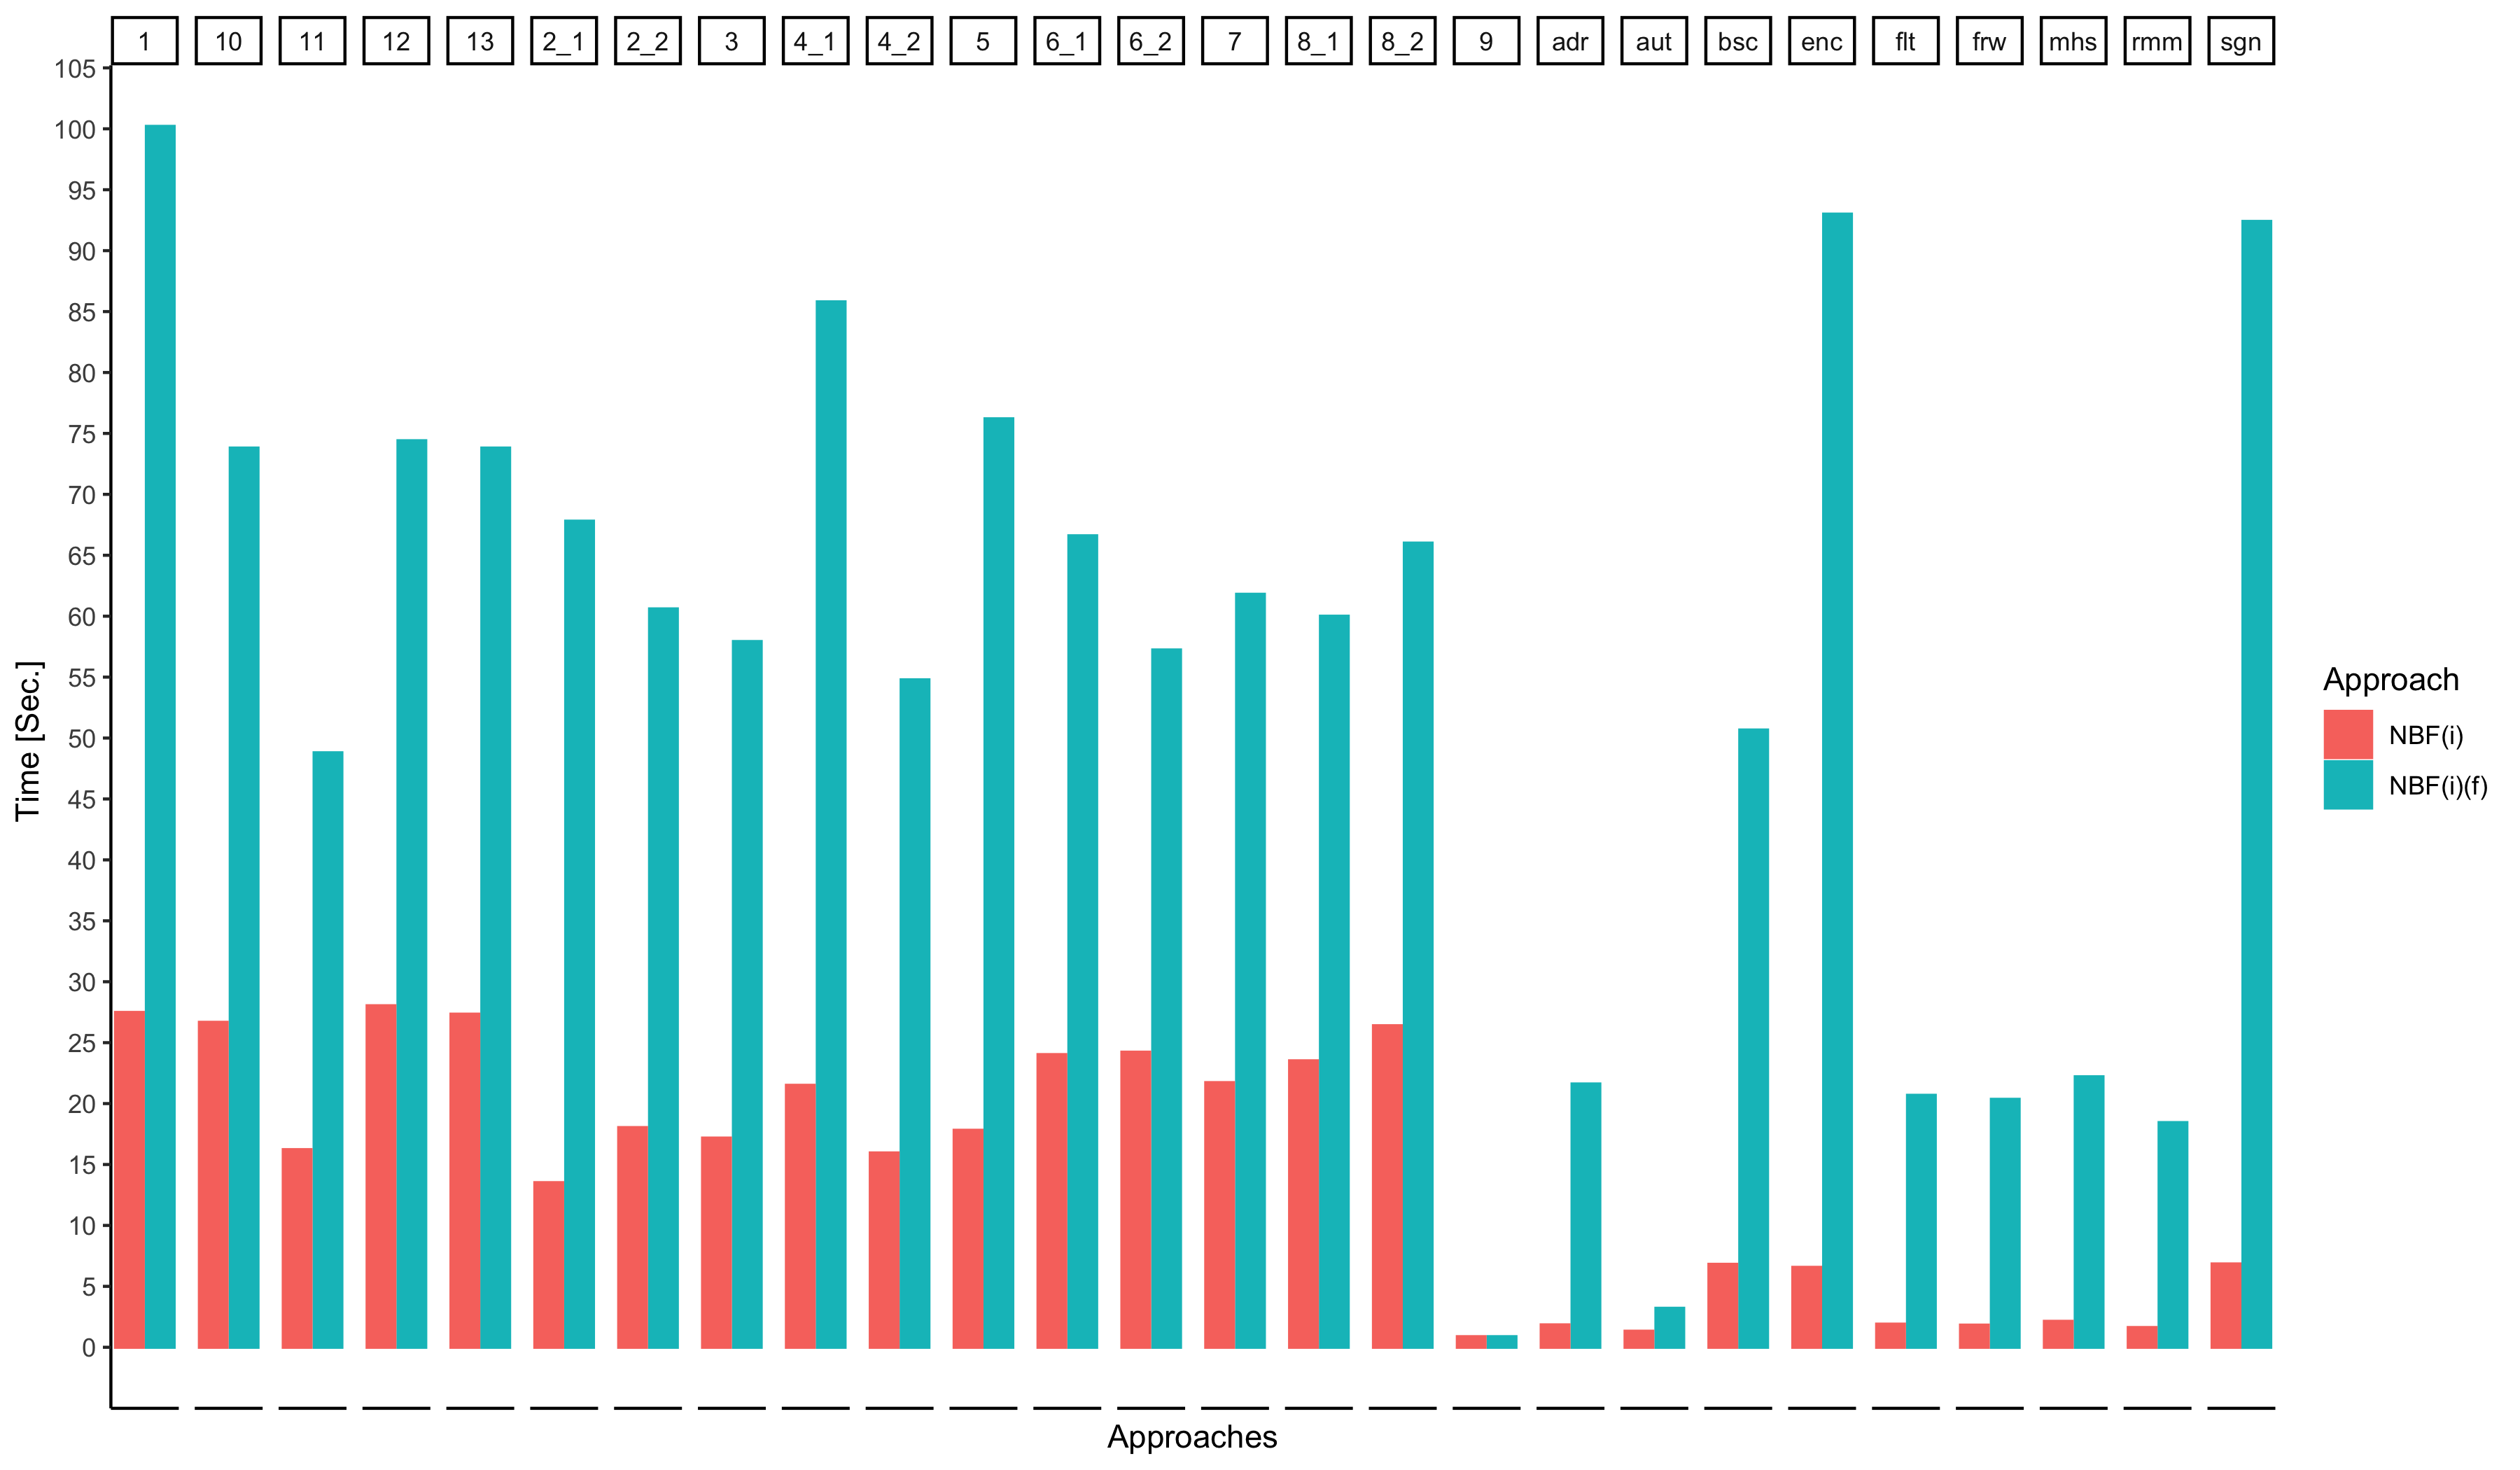
\includegraphics[width=\textwidth]{figs/plots/enron-nbfi-comp-f.png}
        \caption[The \nbfi\ approach versus \nbfif]{The \nbfi\ approach versus \nbfif.}
    \end{subfigure}%
    ~ 
    \begin{subfigure}[t]{0.5\textwidth}
        \centering
        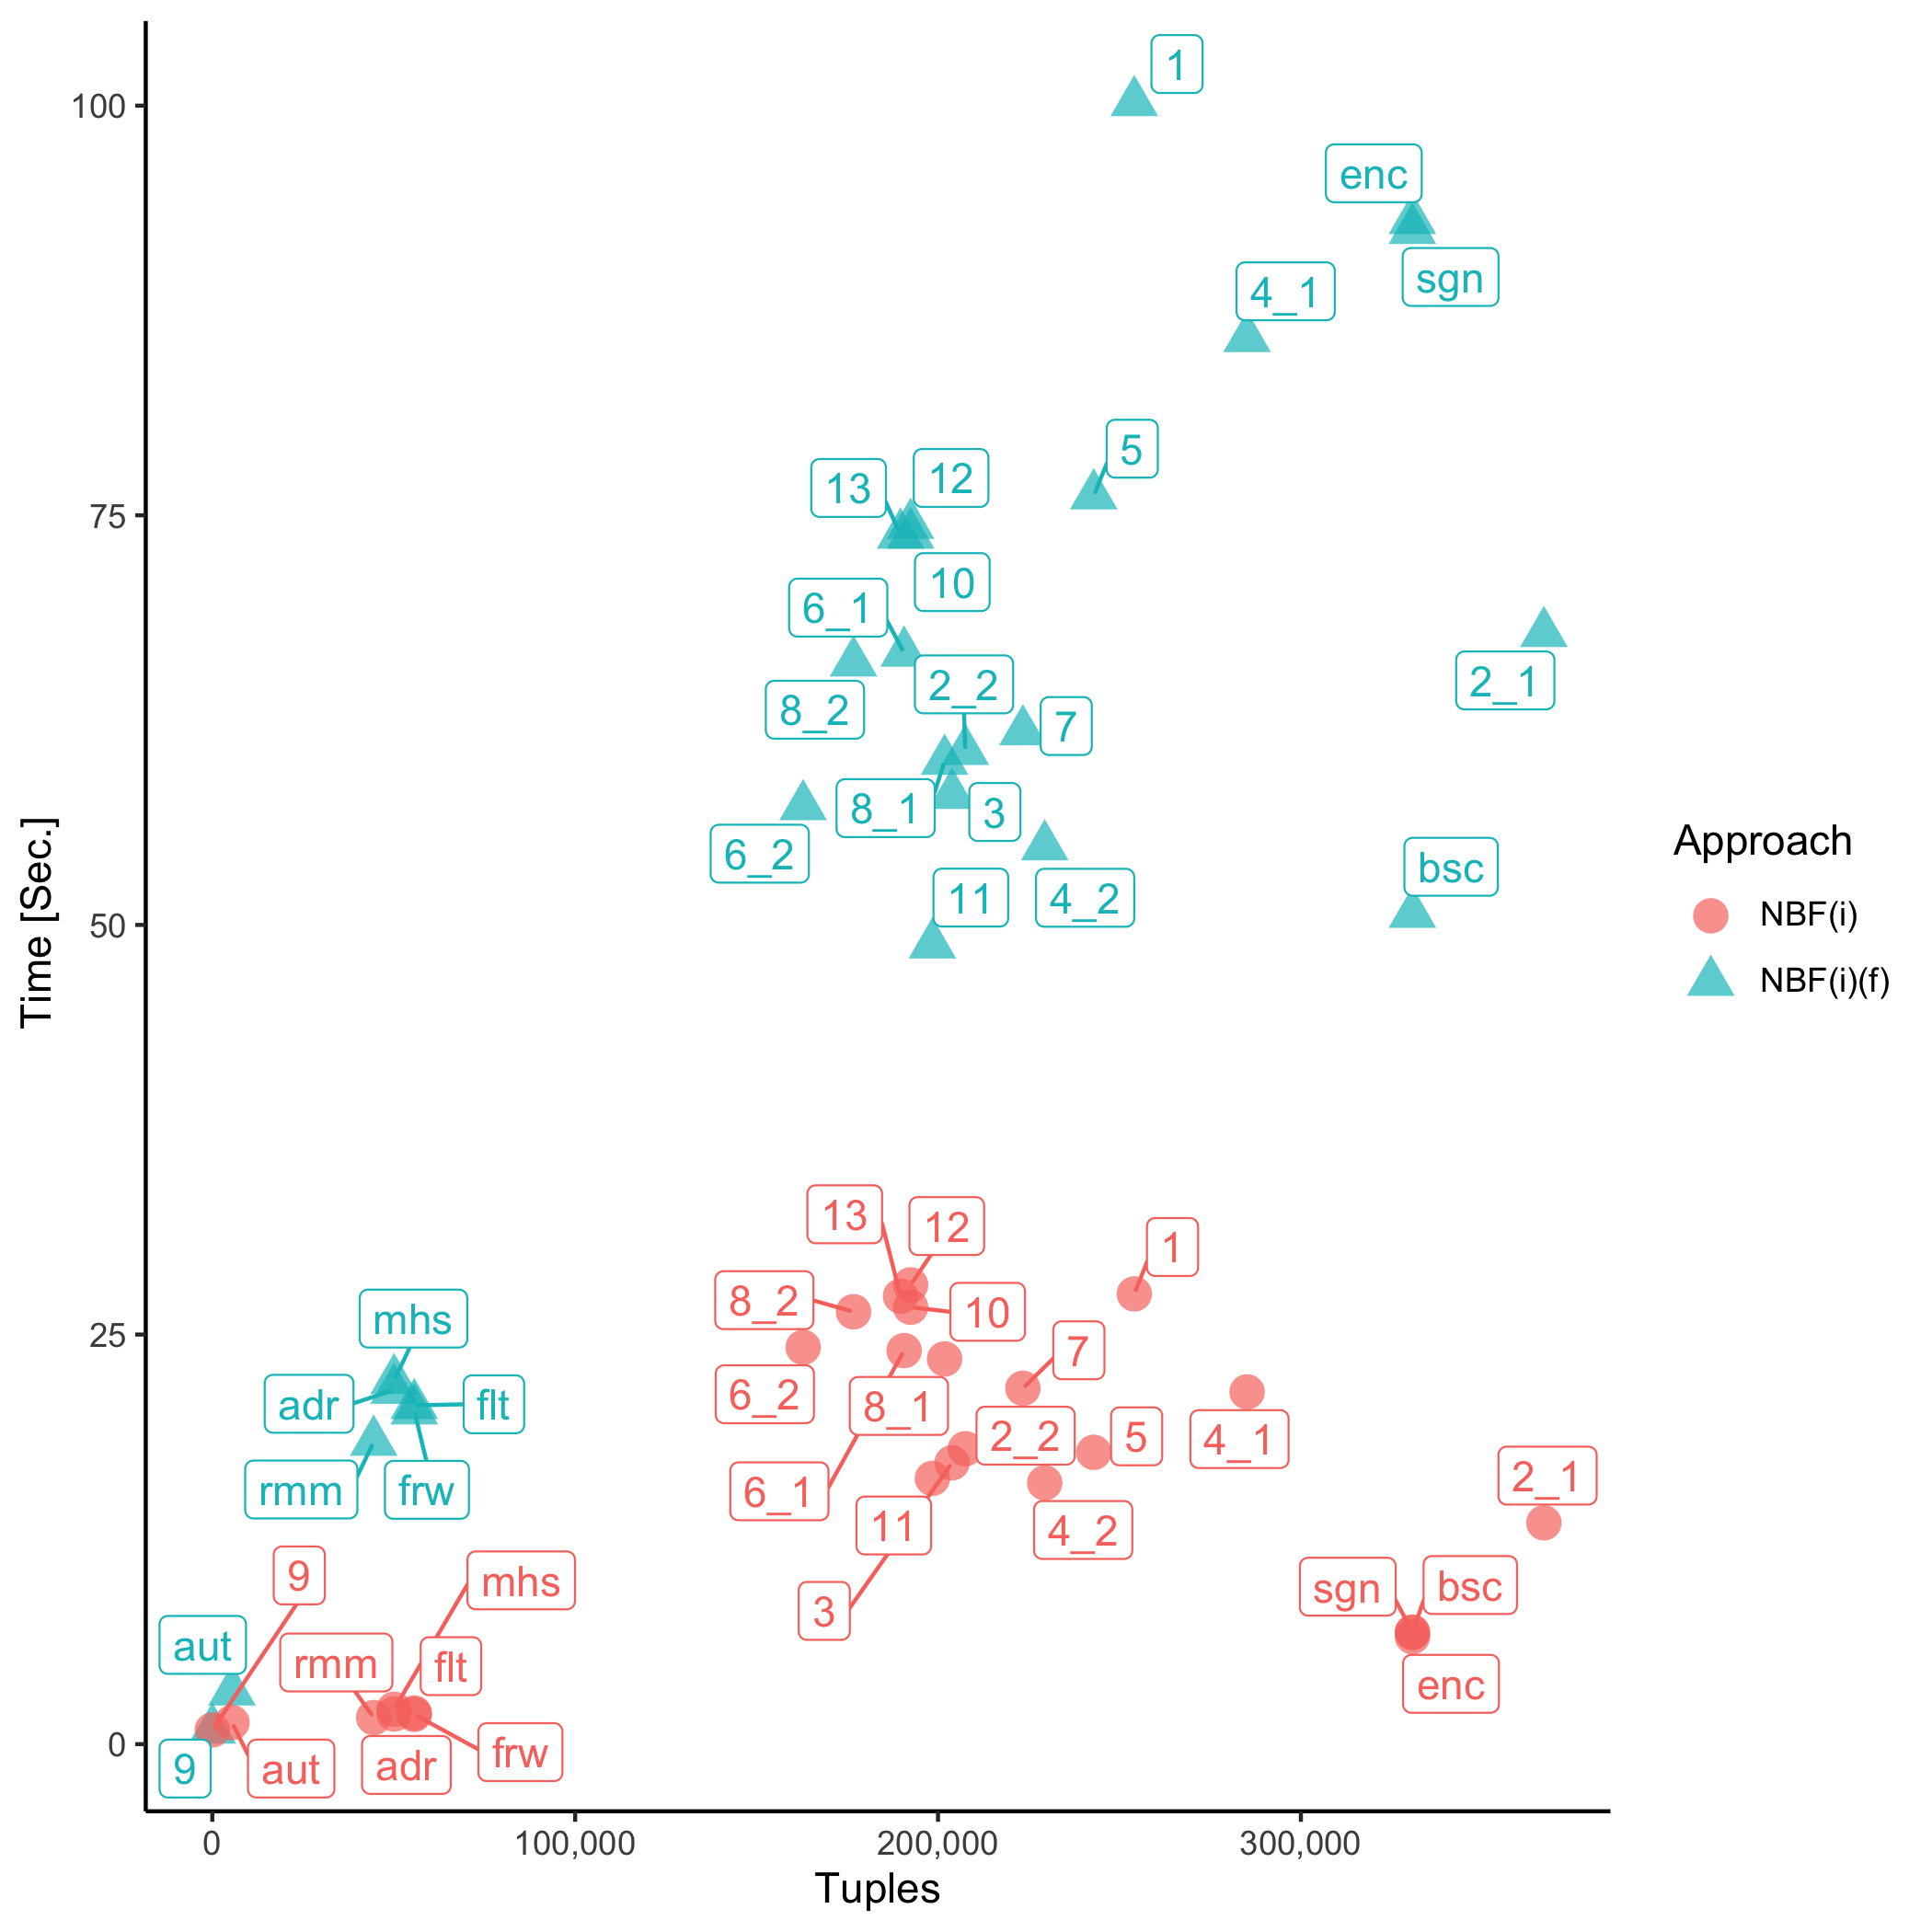
\includegraphics[scale=0.09]{figs/plots/enron-nbfi-f-comp-scatter.png}
        \caption[The \nbfi\ approach versus \nbfif\ as the number of returned tuples increases]{The \nbfi\ approach versus \nbfif\ as the number of returned tuples increases.}
        \label{fig:enron-nbfi-tuple}
    \end{subfigure}\\[1ex]
     \begin{subfigure}[t]{0.5\textwidth}
        \centering
        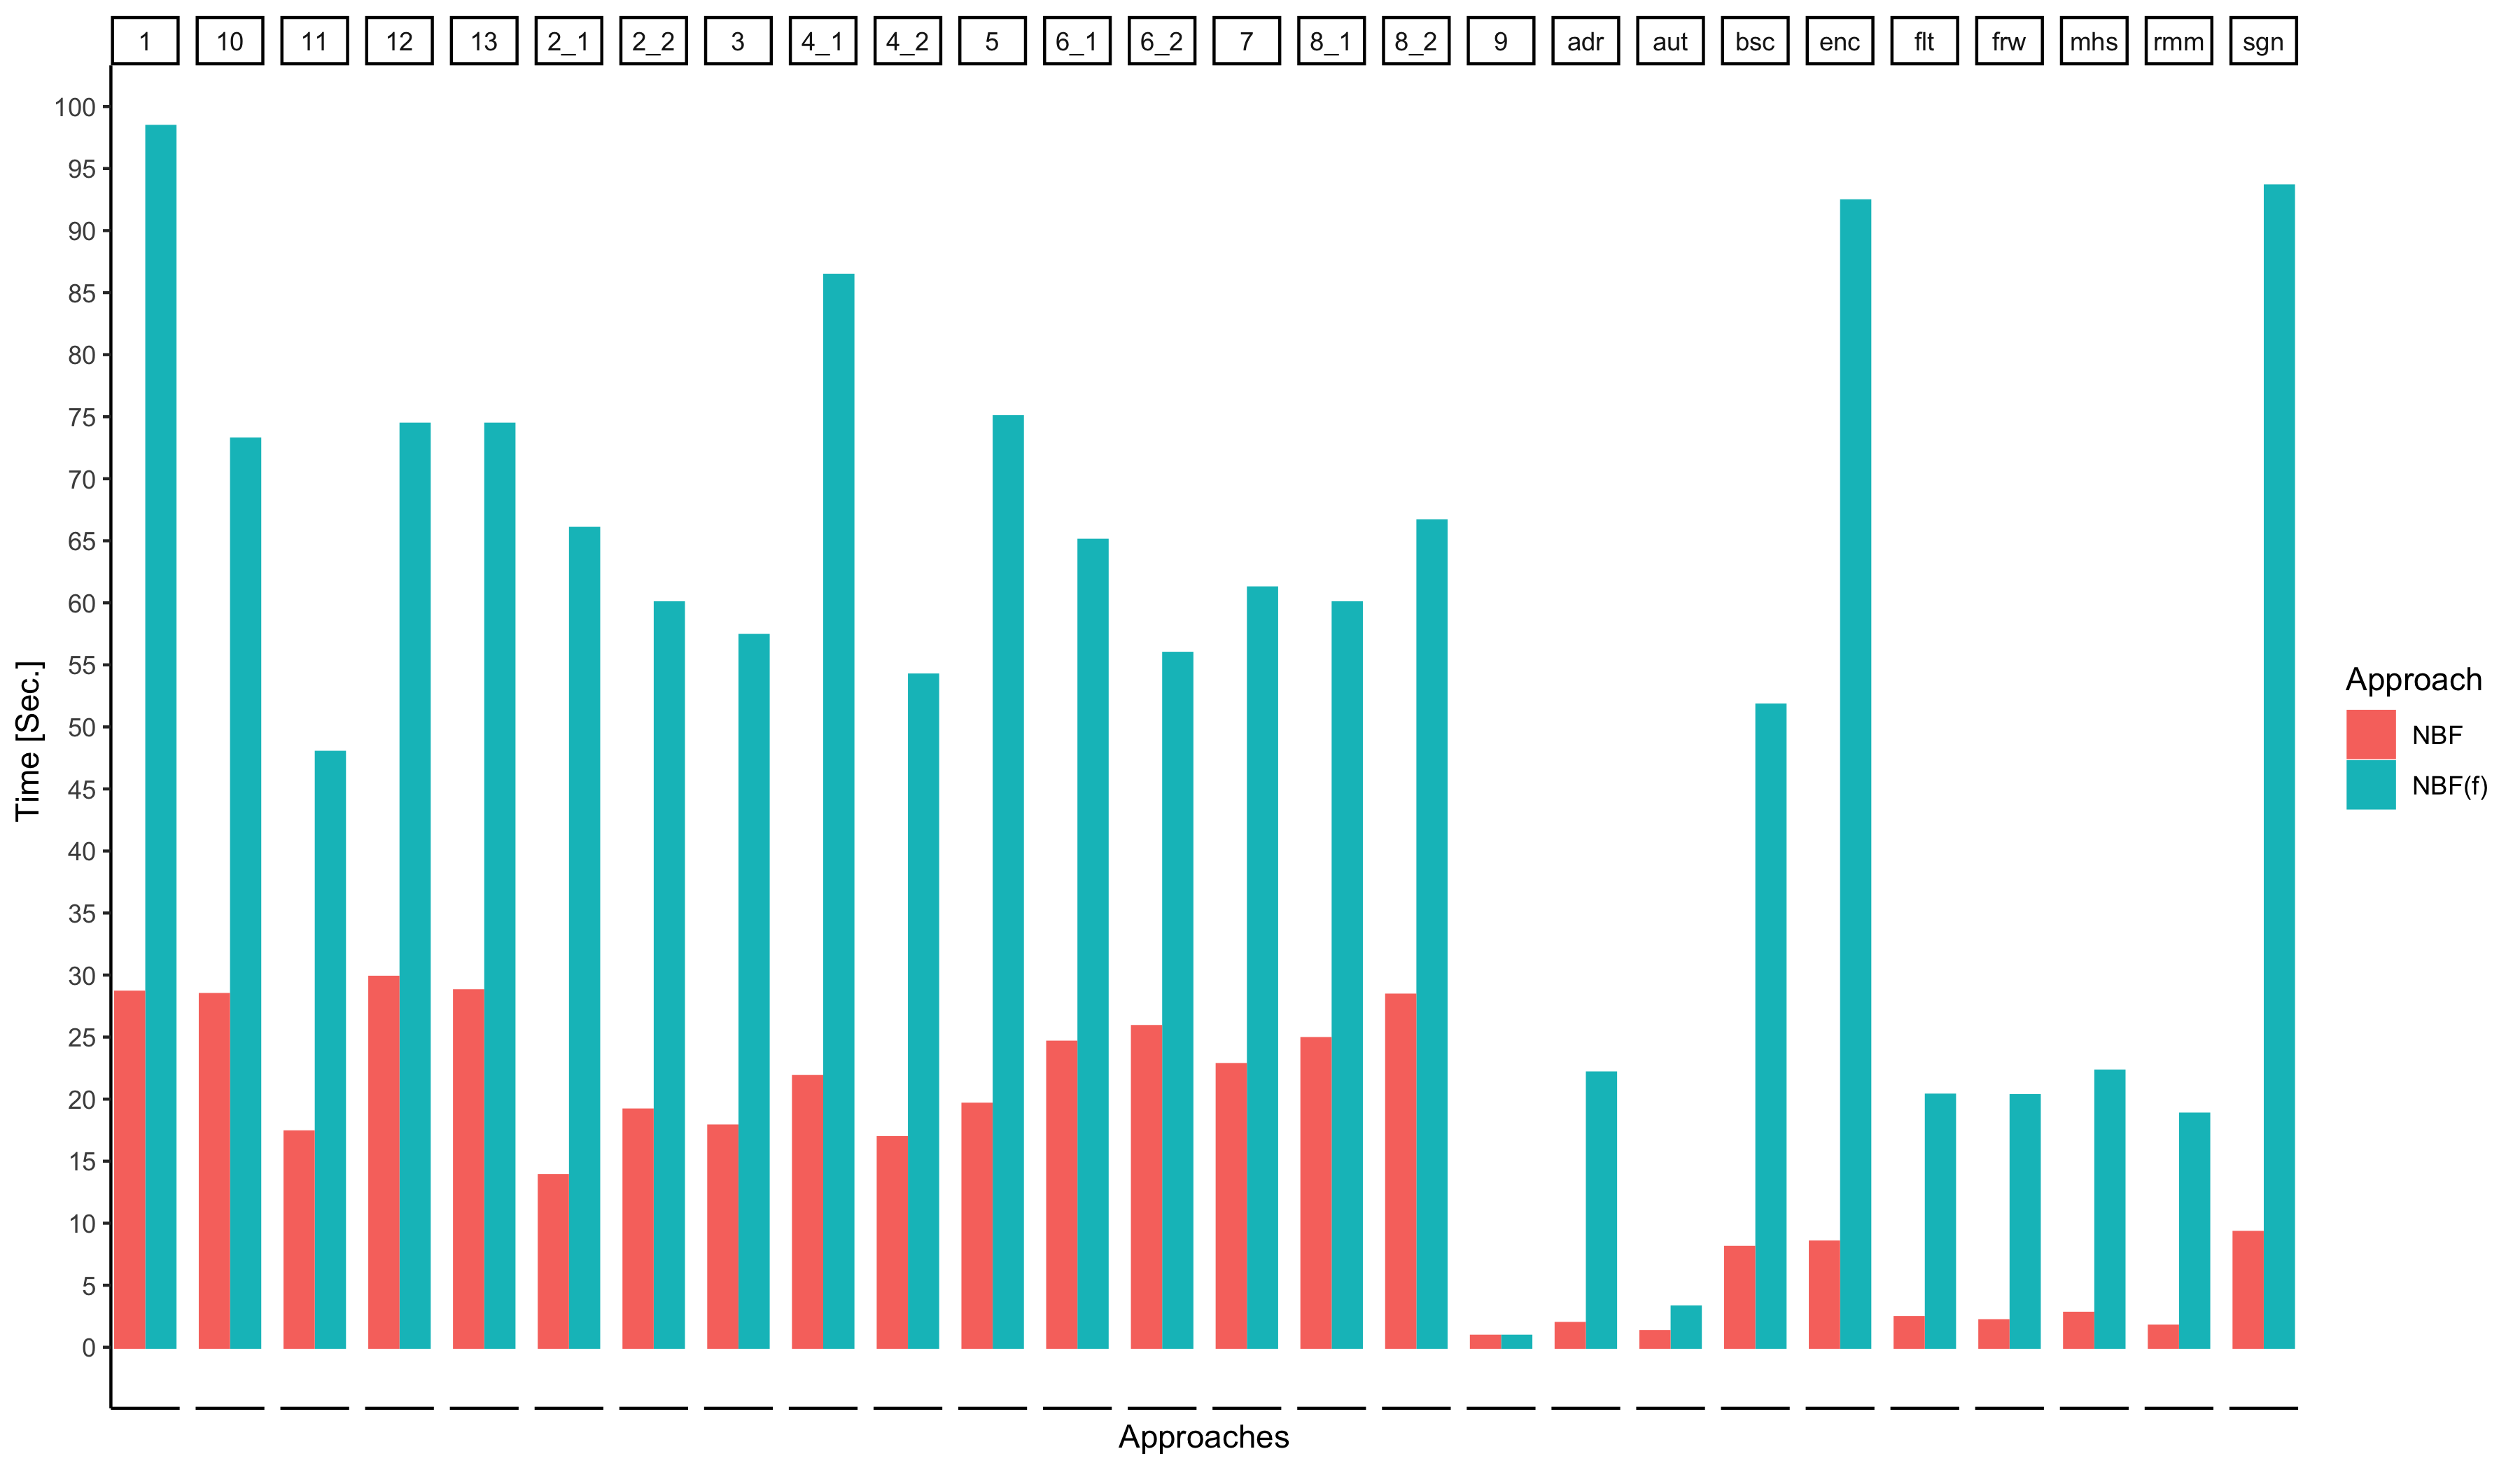
\includegraphics[width=\textwidth]{figs/plots/enron-nbf-comp-f.png}
        \caption[The \nbf\ approach versus \nbff]{The \nbf\ approach versus \nbff.}
    \end{subfigure}%
    ~ 
    \begin{subfigure}[t]{0.5\textwidth}
        \centering
        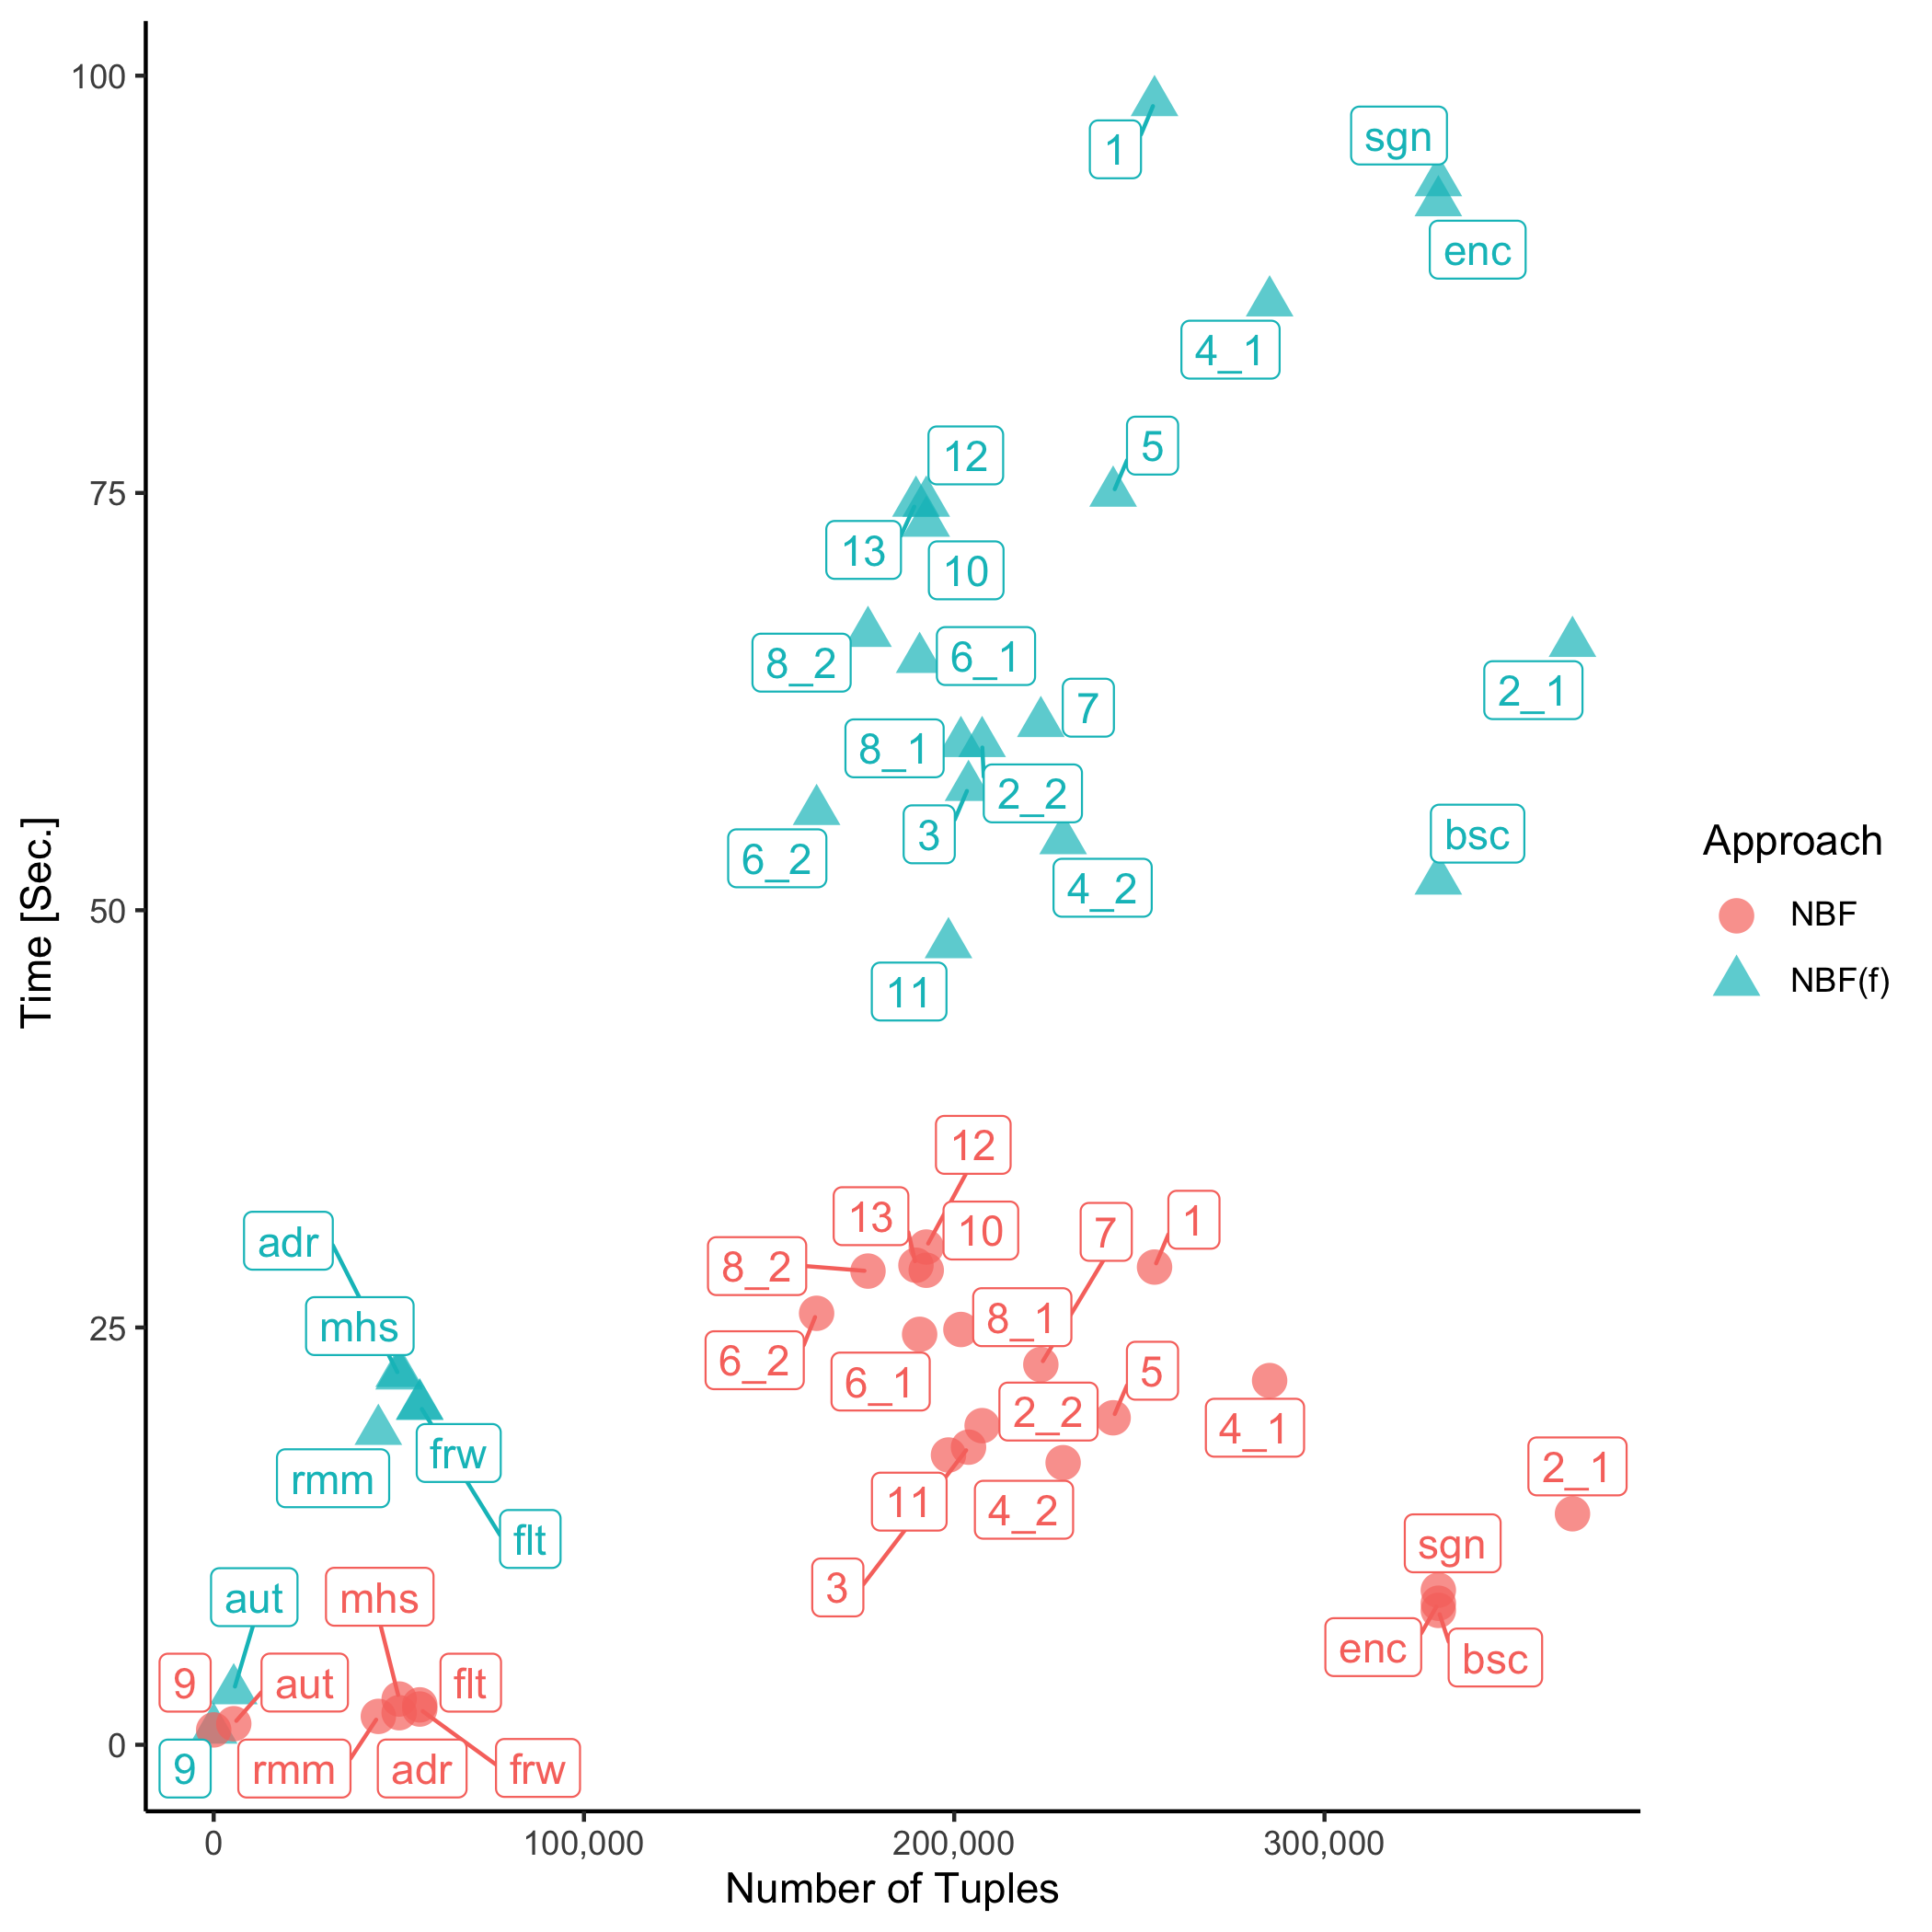
\includegraphics[scale=0.09]{figs/plots/enron-nbf-f-comp-scatter.png}
        \caption[The \nbf\ approach versus \nbff\ as the number of returned tuples increases]{The \nbf\ approach versus \nbff\ as the number of returned tuples increases.}
        \label{fig:enron-nbf-tuple}
    \end{subfigure}
    \caption[The effect of filtering out tuples with unsatisfiable presence conditions on SQL generator 
    approaches over the email VDB]{The effect of filtering out tuples with unsatisfiable presence conditions on SQL generator 
    approaches over the email VDB.}
    \label{fig:enron-nbfs-filter}
\end{figure*}

%\begin{figure*}[t!]
%    \centering
%    \begin{subfigure}[t]{0.5\textwidth}
%        \centering
%        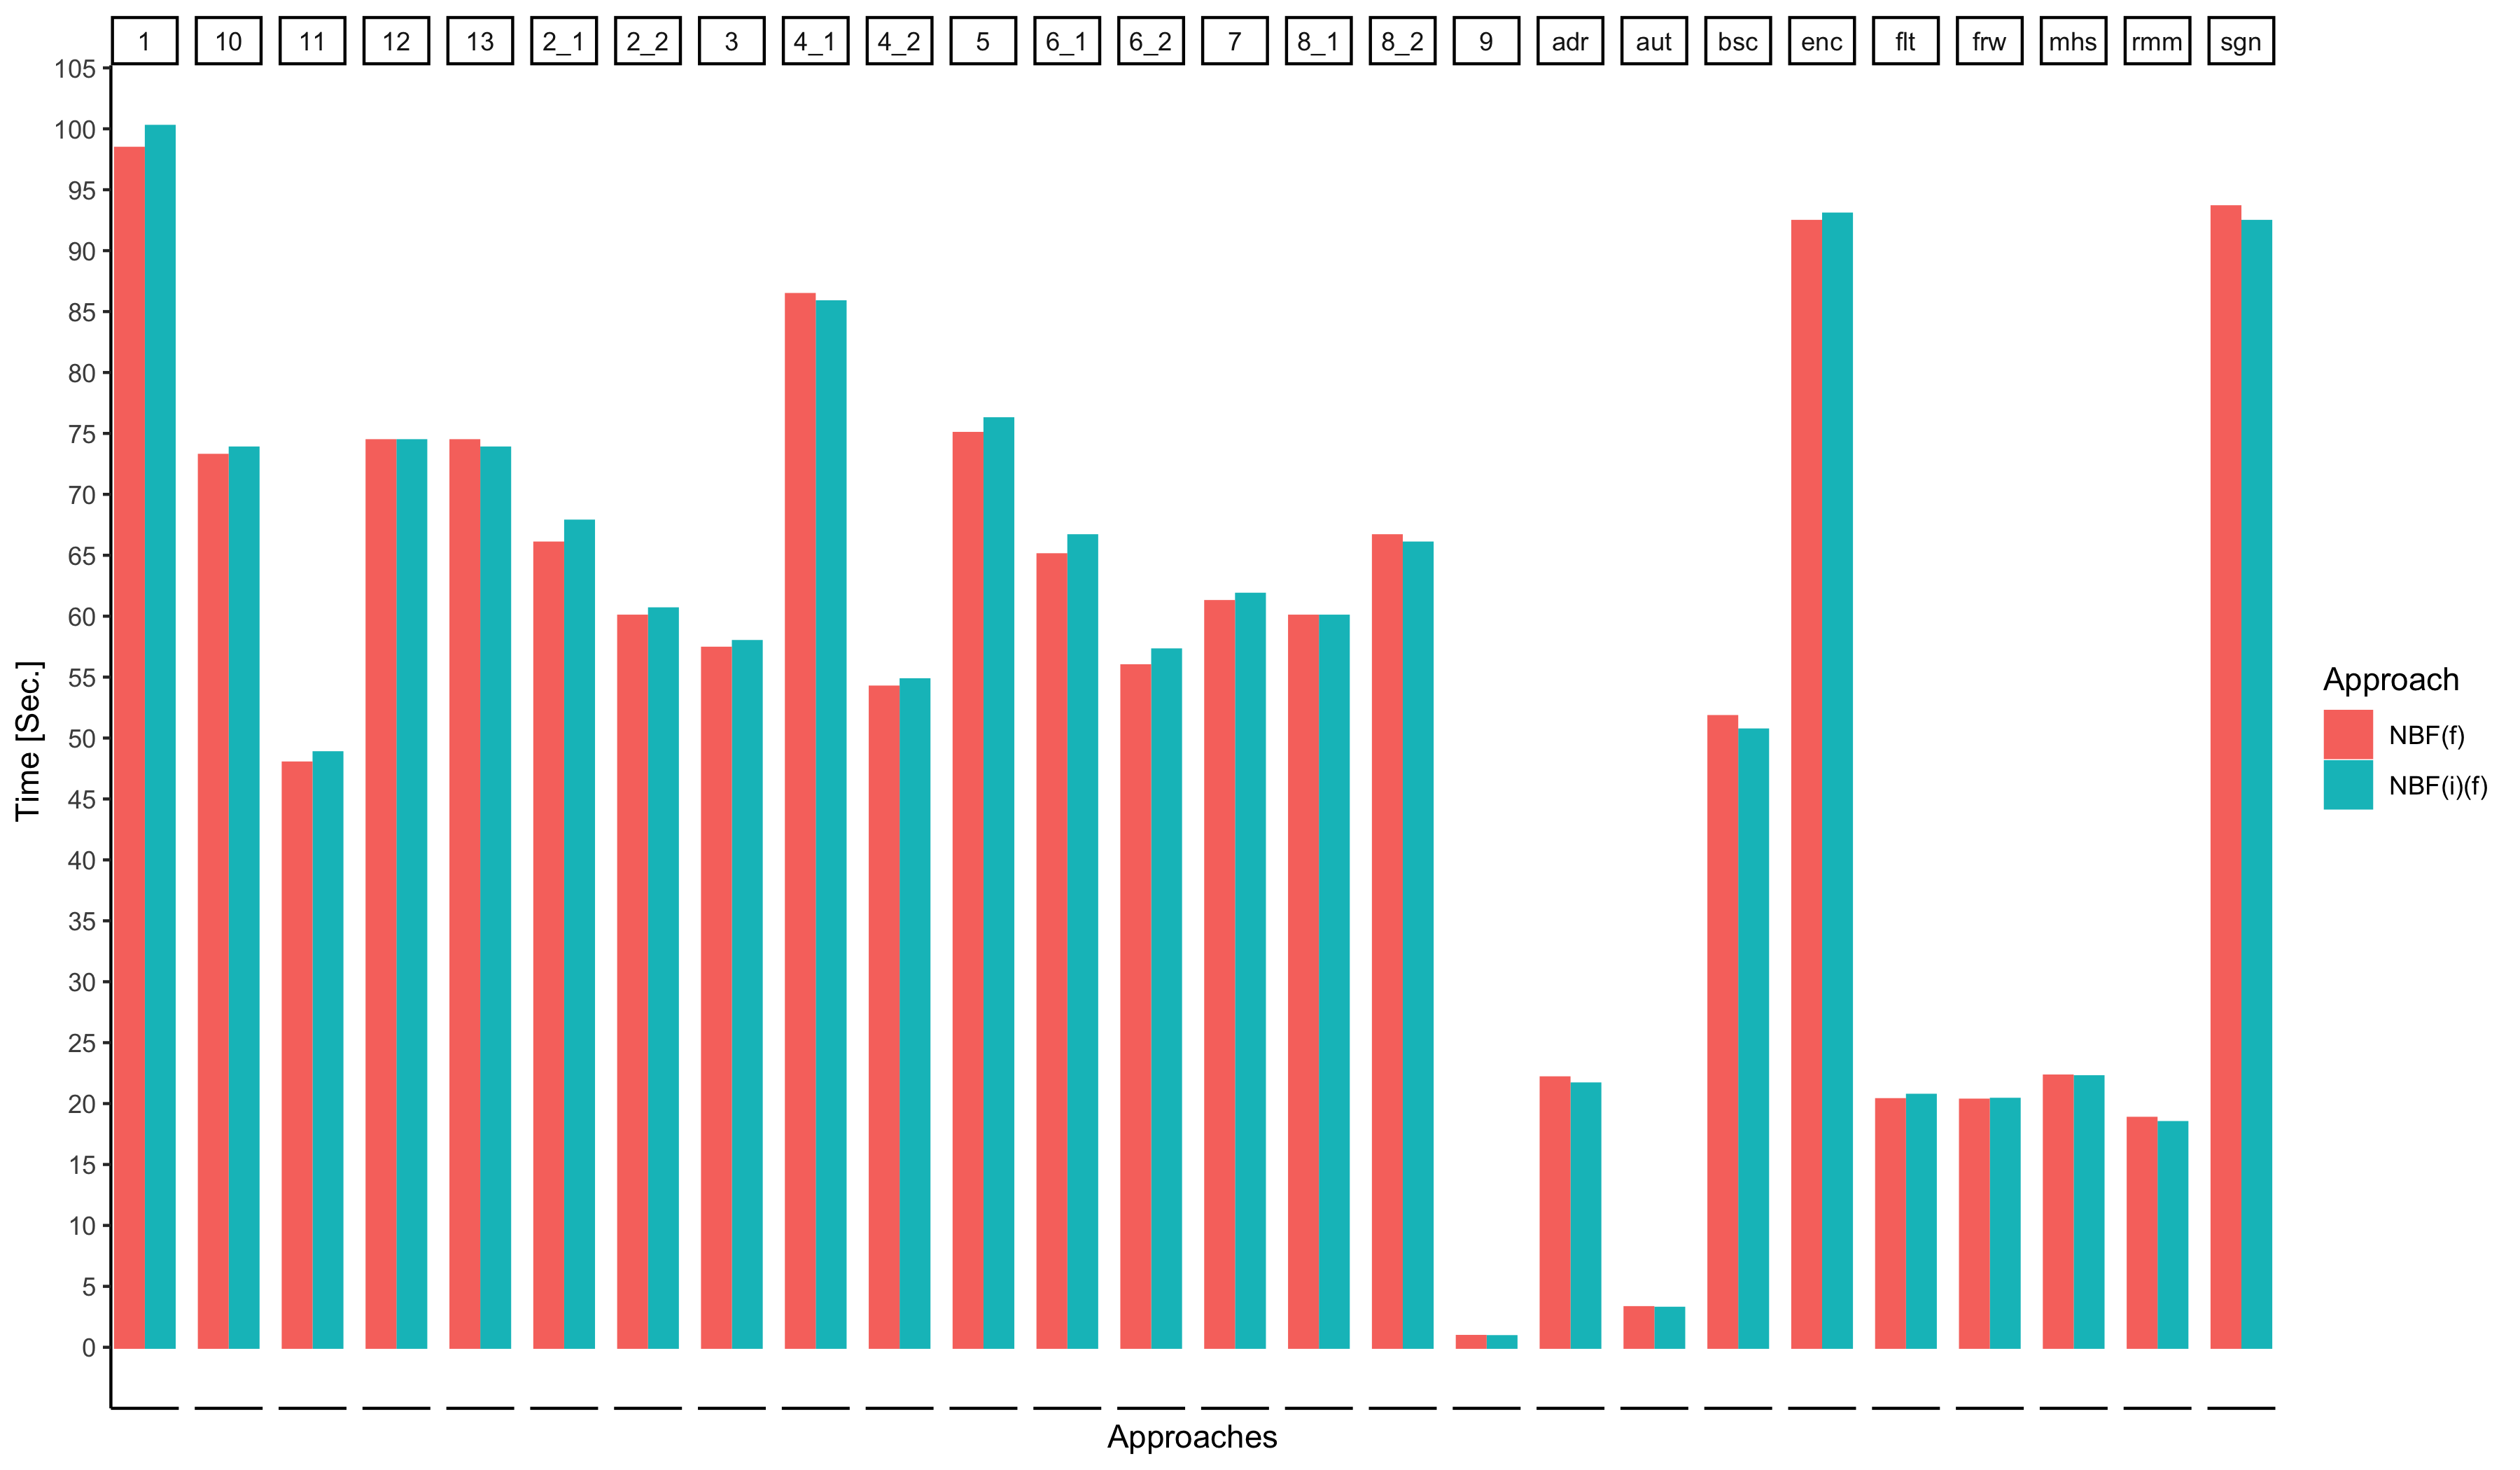
\includegraphics[width=\textwidth]{figs/plots/enron-nbf-f.png}
%        \caption{Lorem ipsum}
%    \end{subfigure}%
%    ~ 
%    \begin{subfigure}[t]{0.5\textwidth}
%        \centering
%        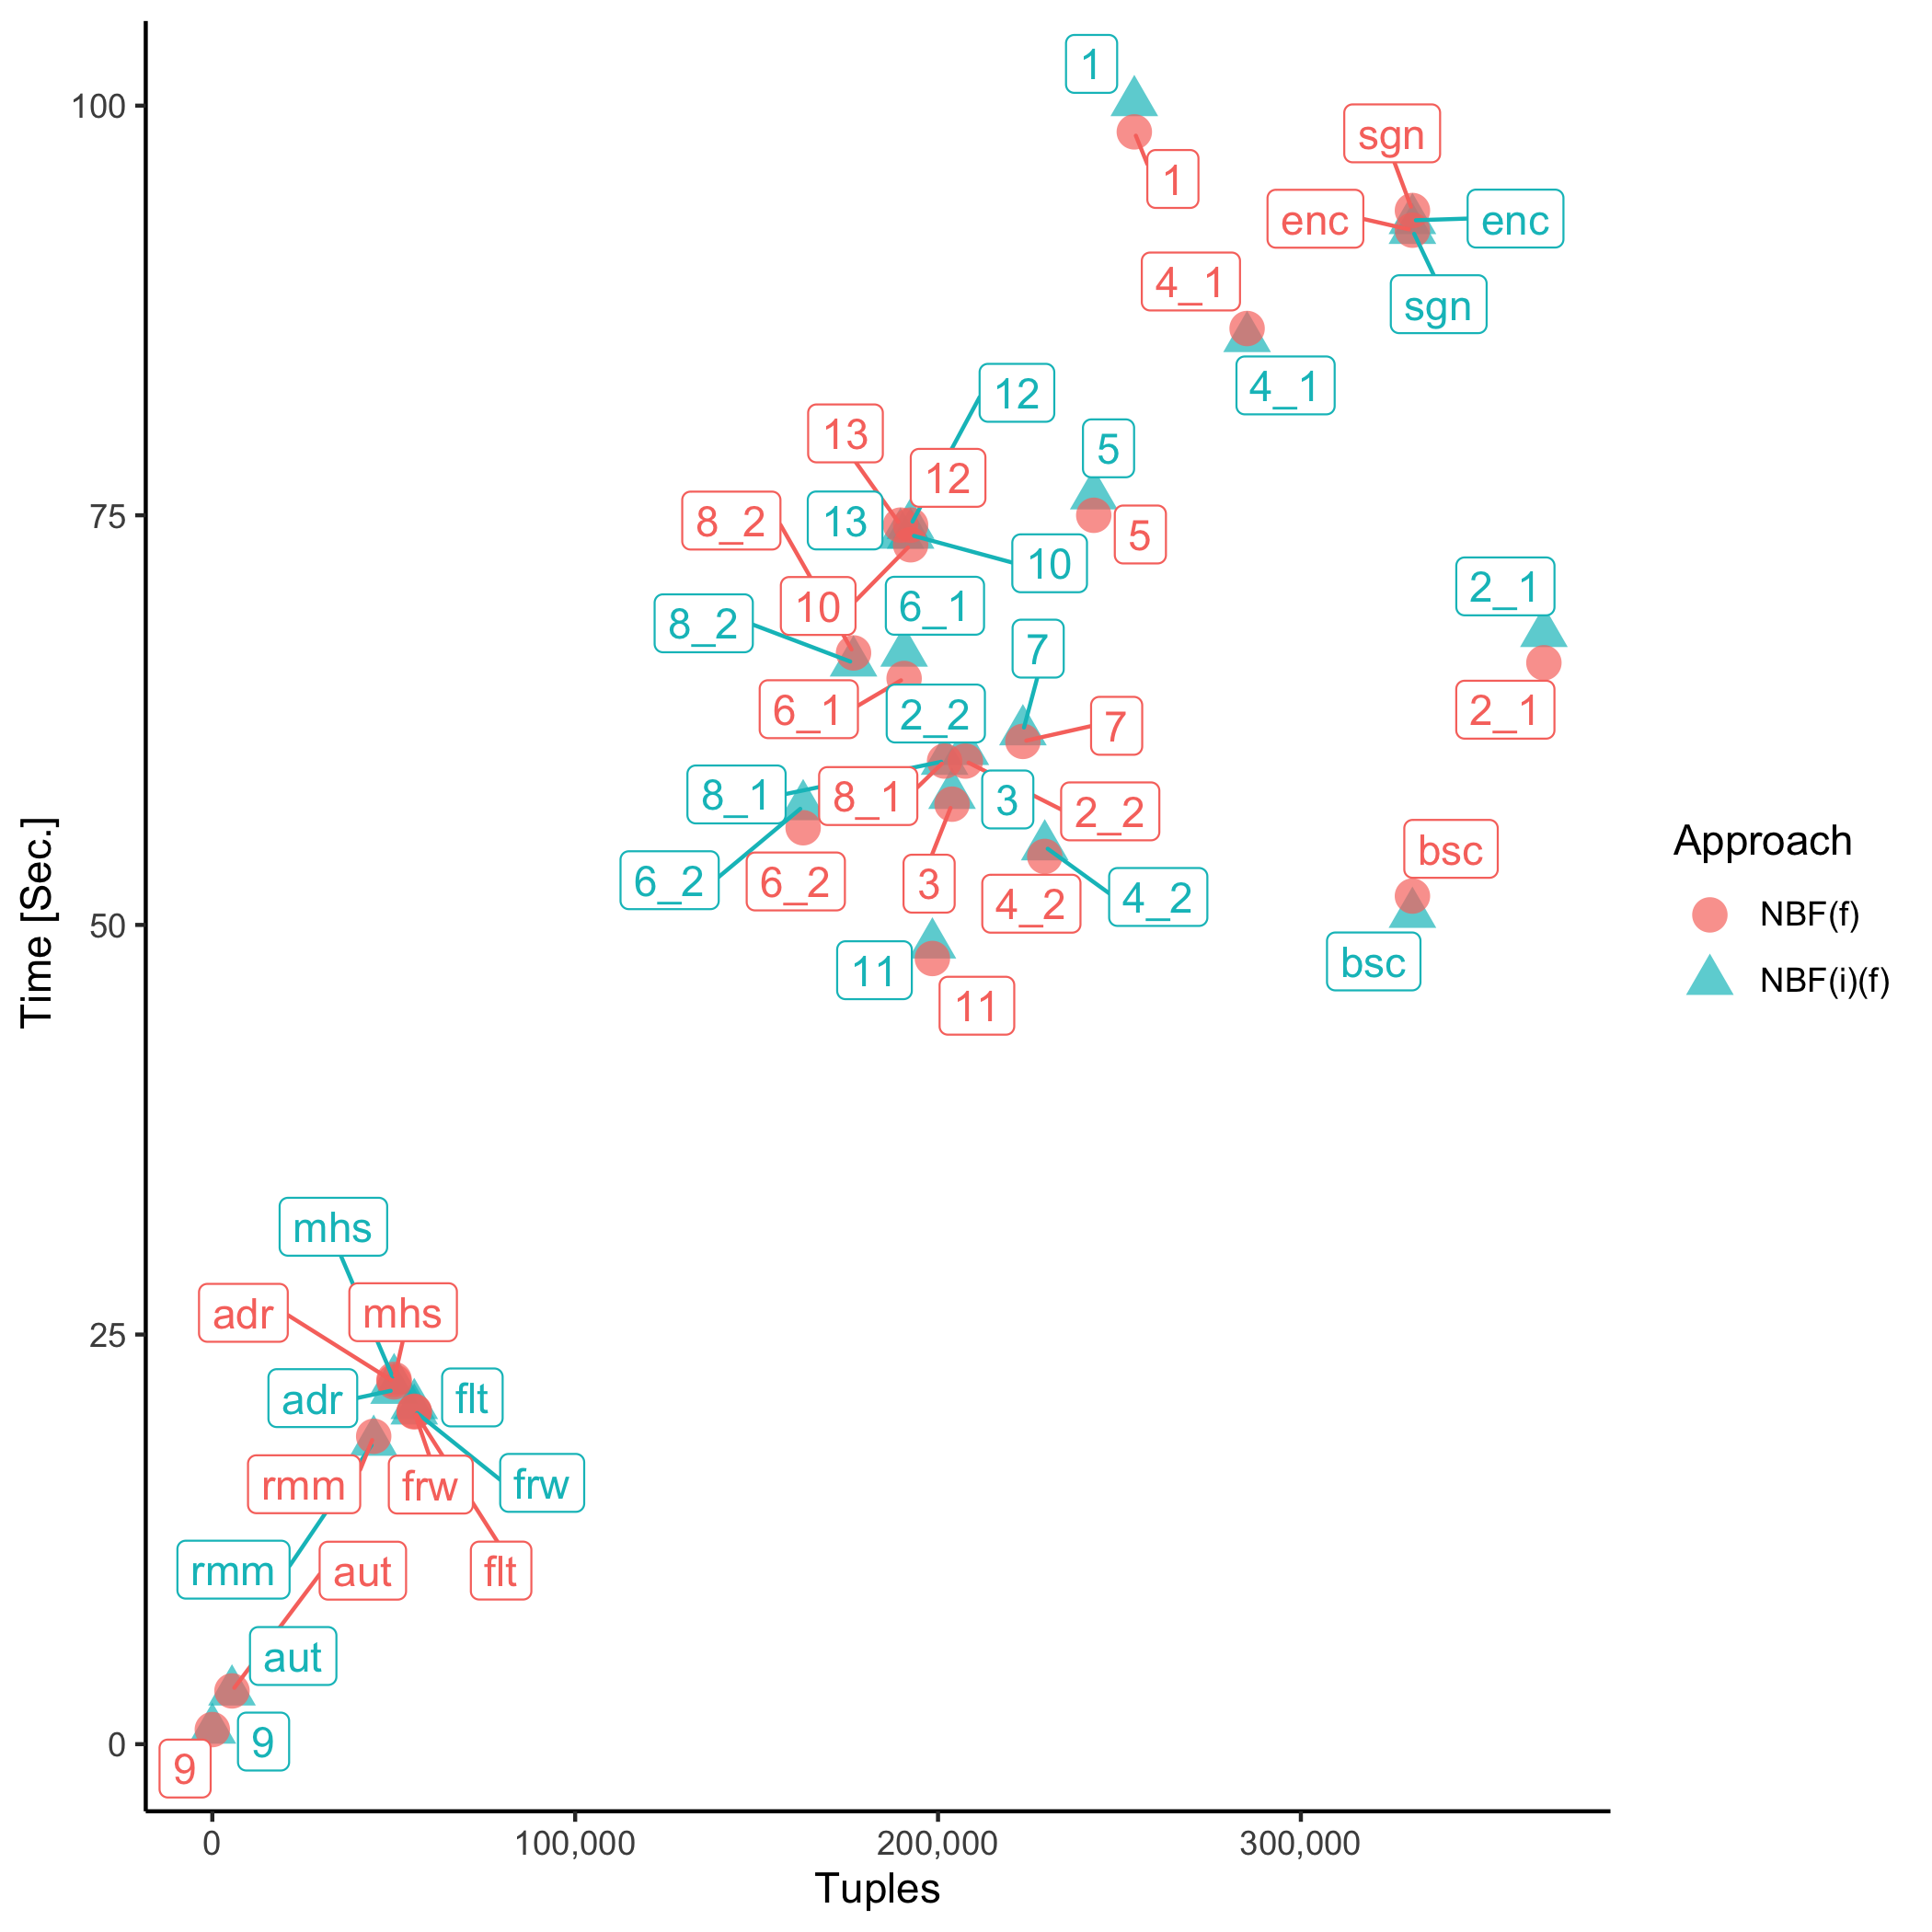
\includegraphics[scale=0.09]{figs/plots/enron-nbf-f-scatter.png}
%        \caption{Lorem ipsum, lorem ipsum,Lorem ipsum, lorem ipsum,Lorem ipsum}
%    \end{subfigure}
%    \caption{Caption place holder}
%\end{figure*}

%\begin{figure*}[t!]
%    \centering
%    \begin{subfigure}[t]{0.5\textwidth}
%        \centering
%        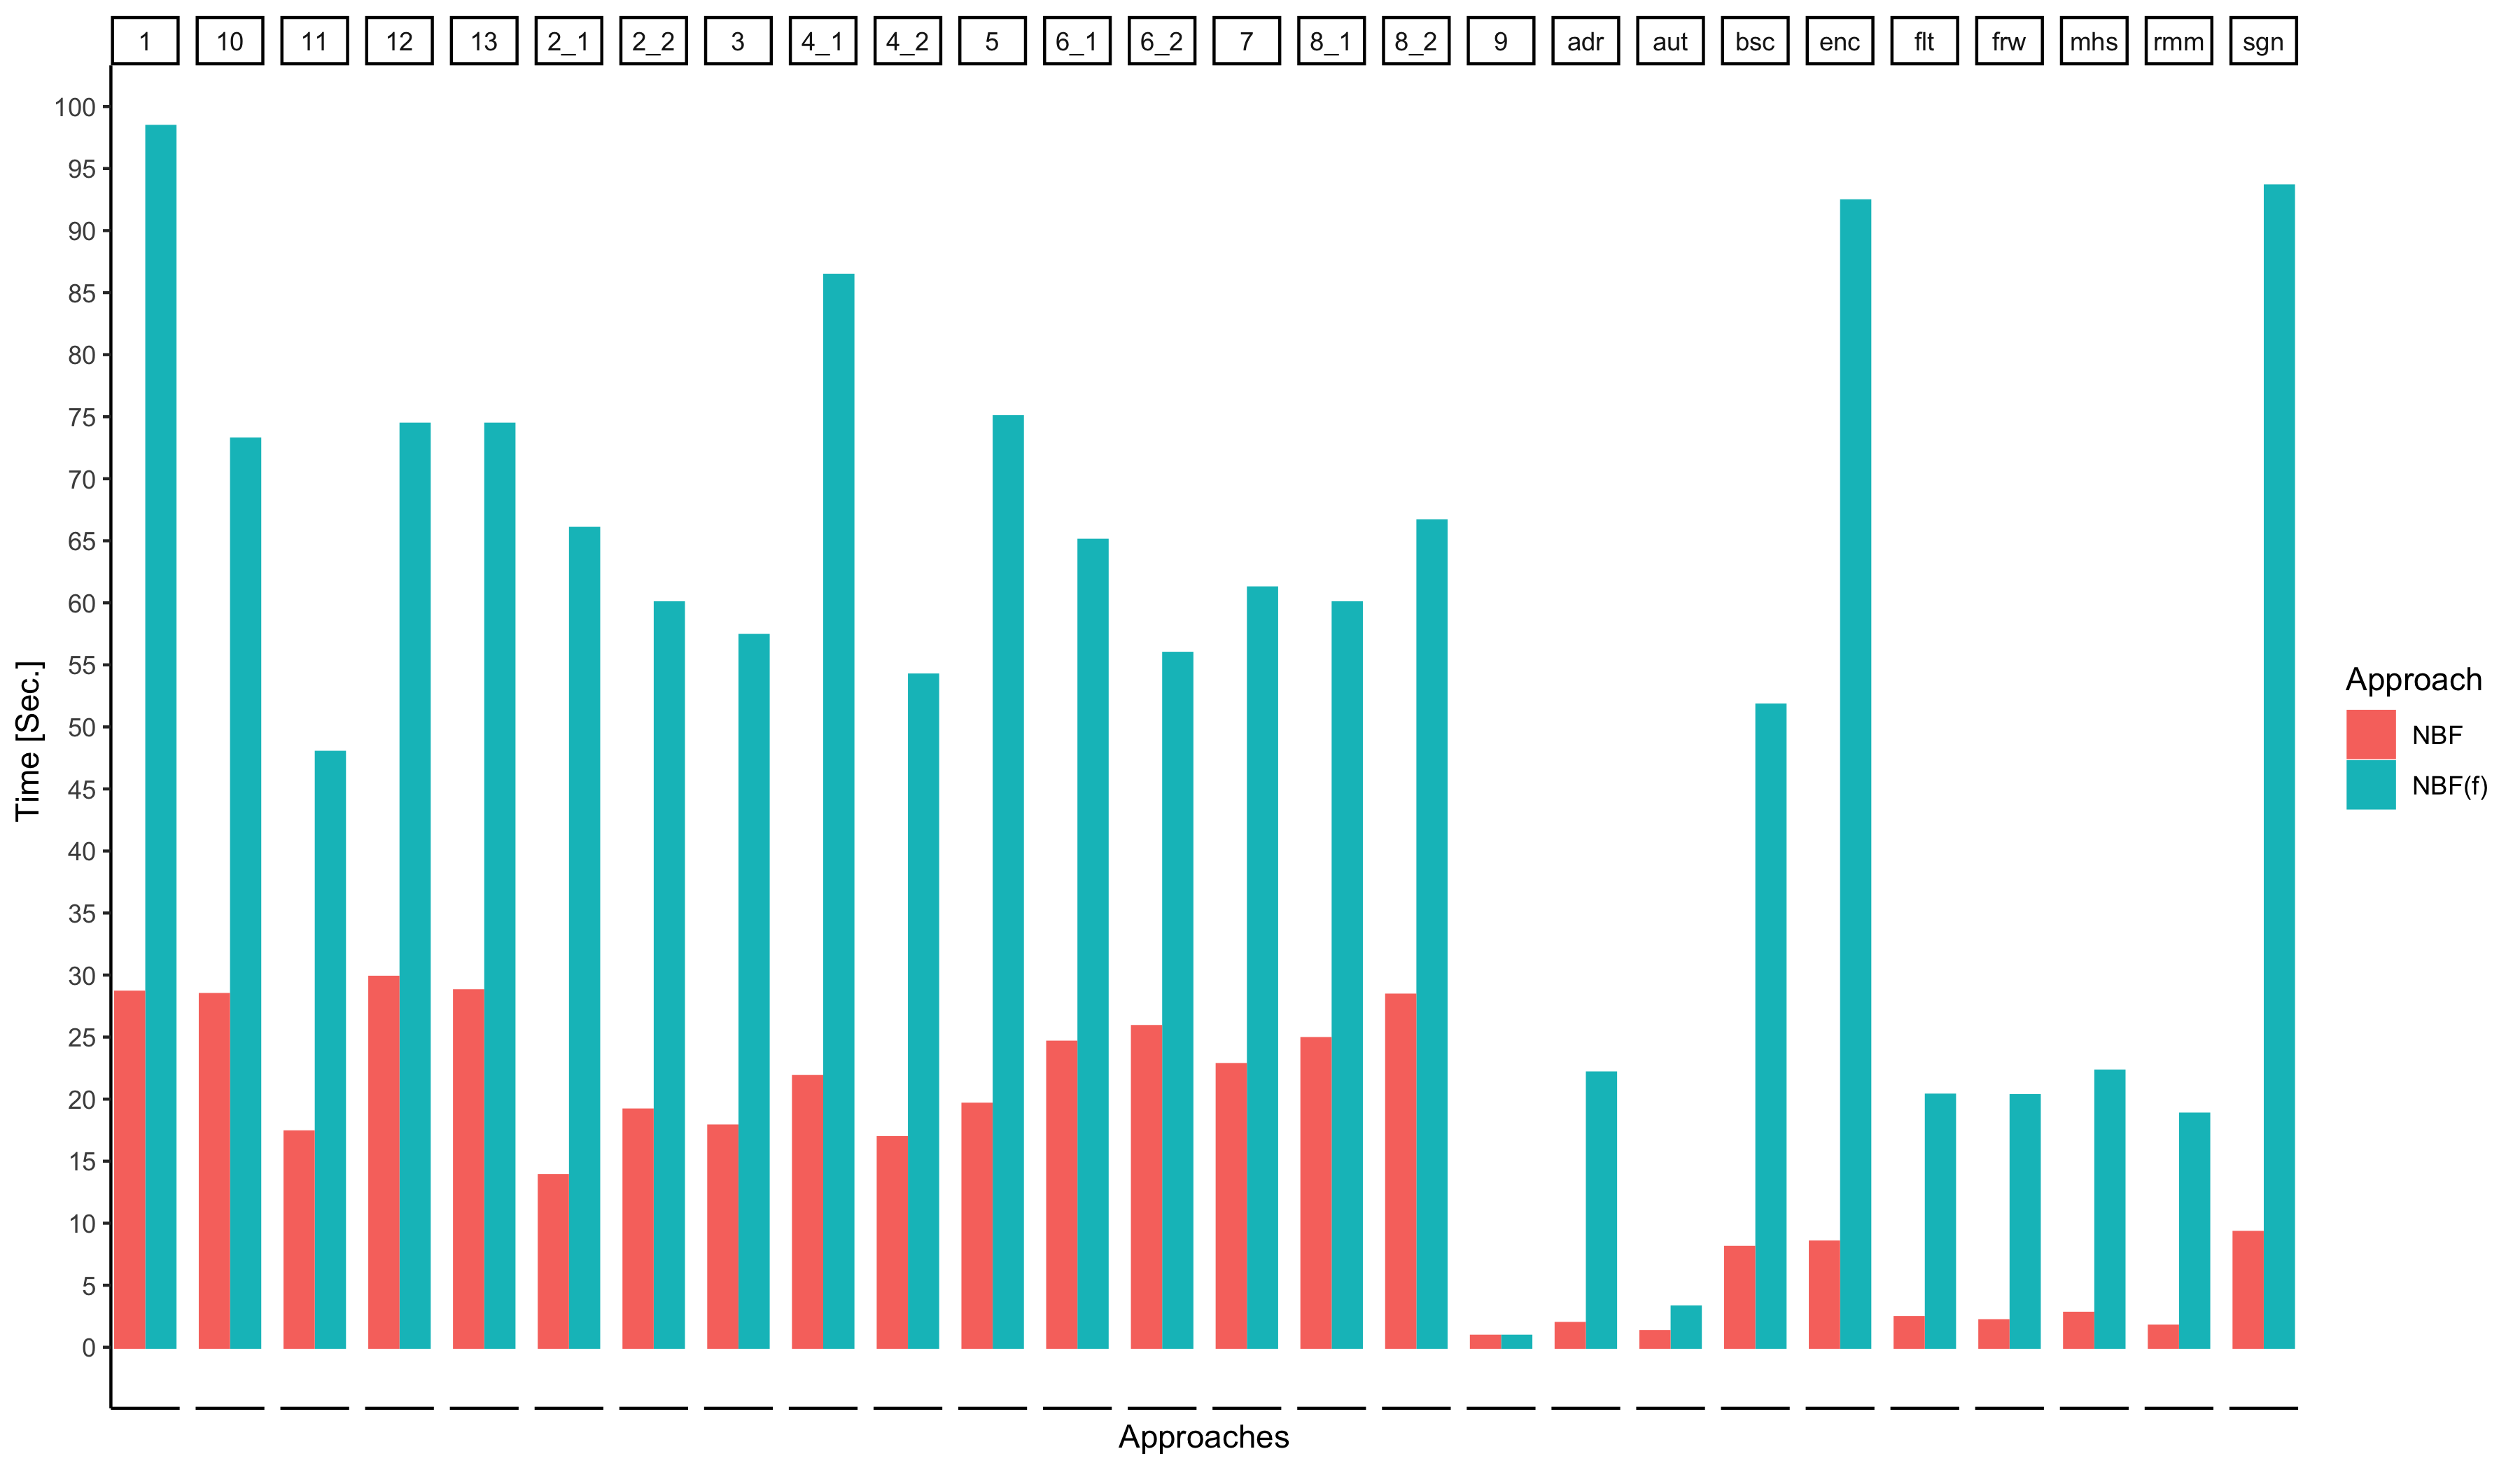
\includegraphics[width=\textwidth]{figs/plots/enron-nbf-comp-f.png}
%        \caption{Lorem ipsum}
%    \end{subfigure}%
%    ~ 
%    \begin{subfigure}[t]{0.5\textwidth}
%        \centering
%        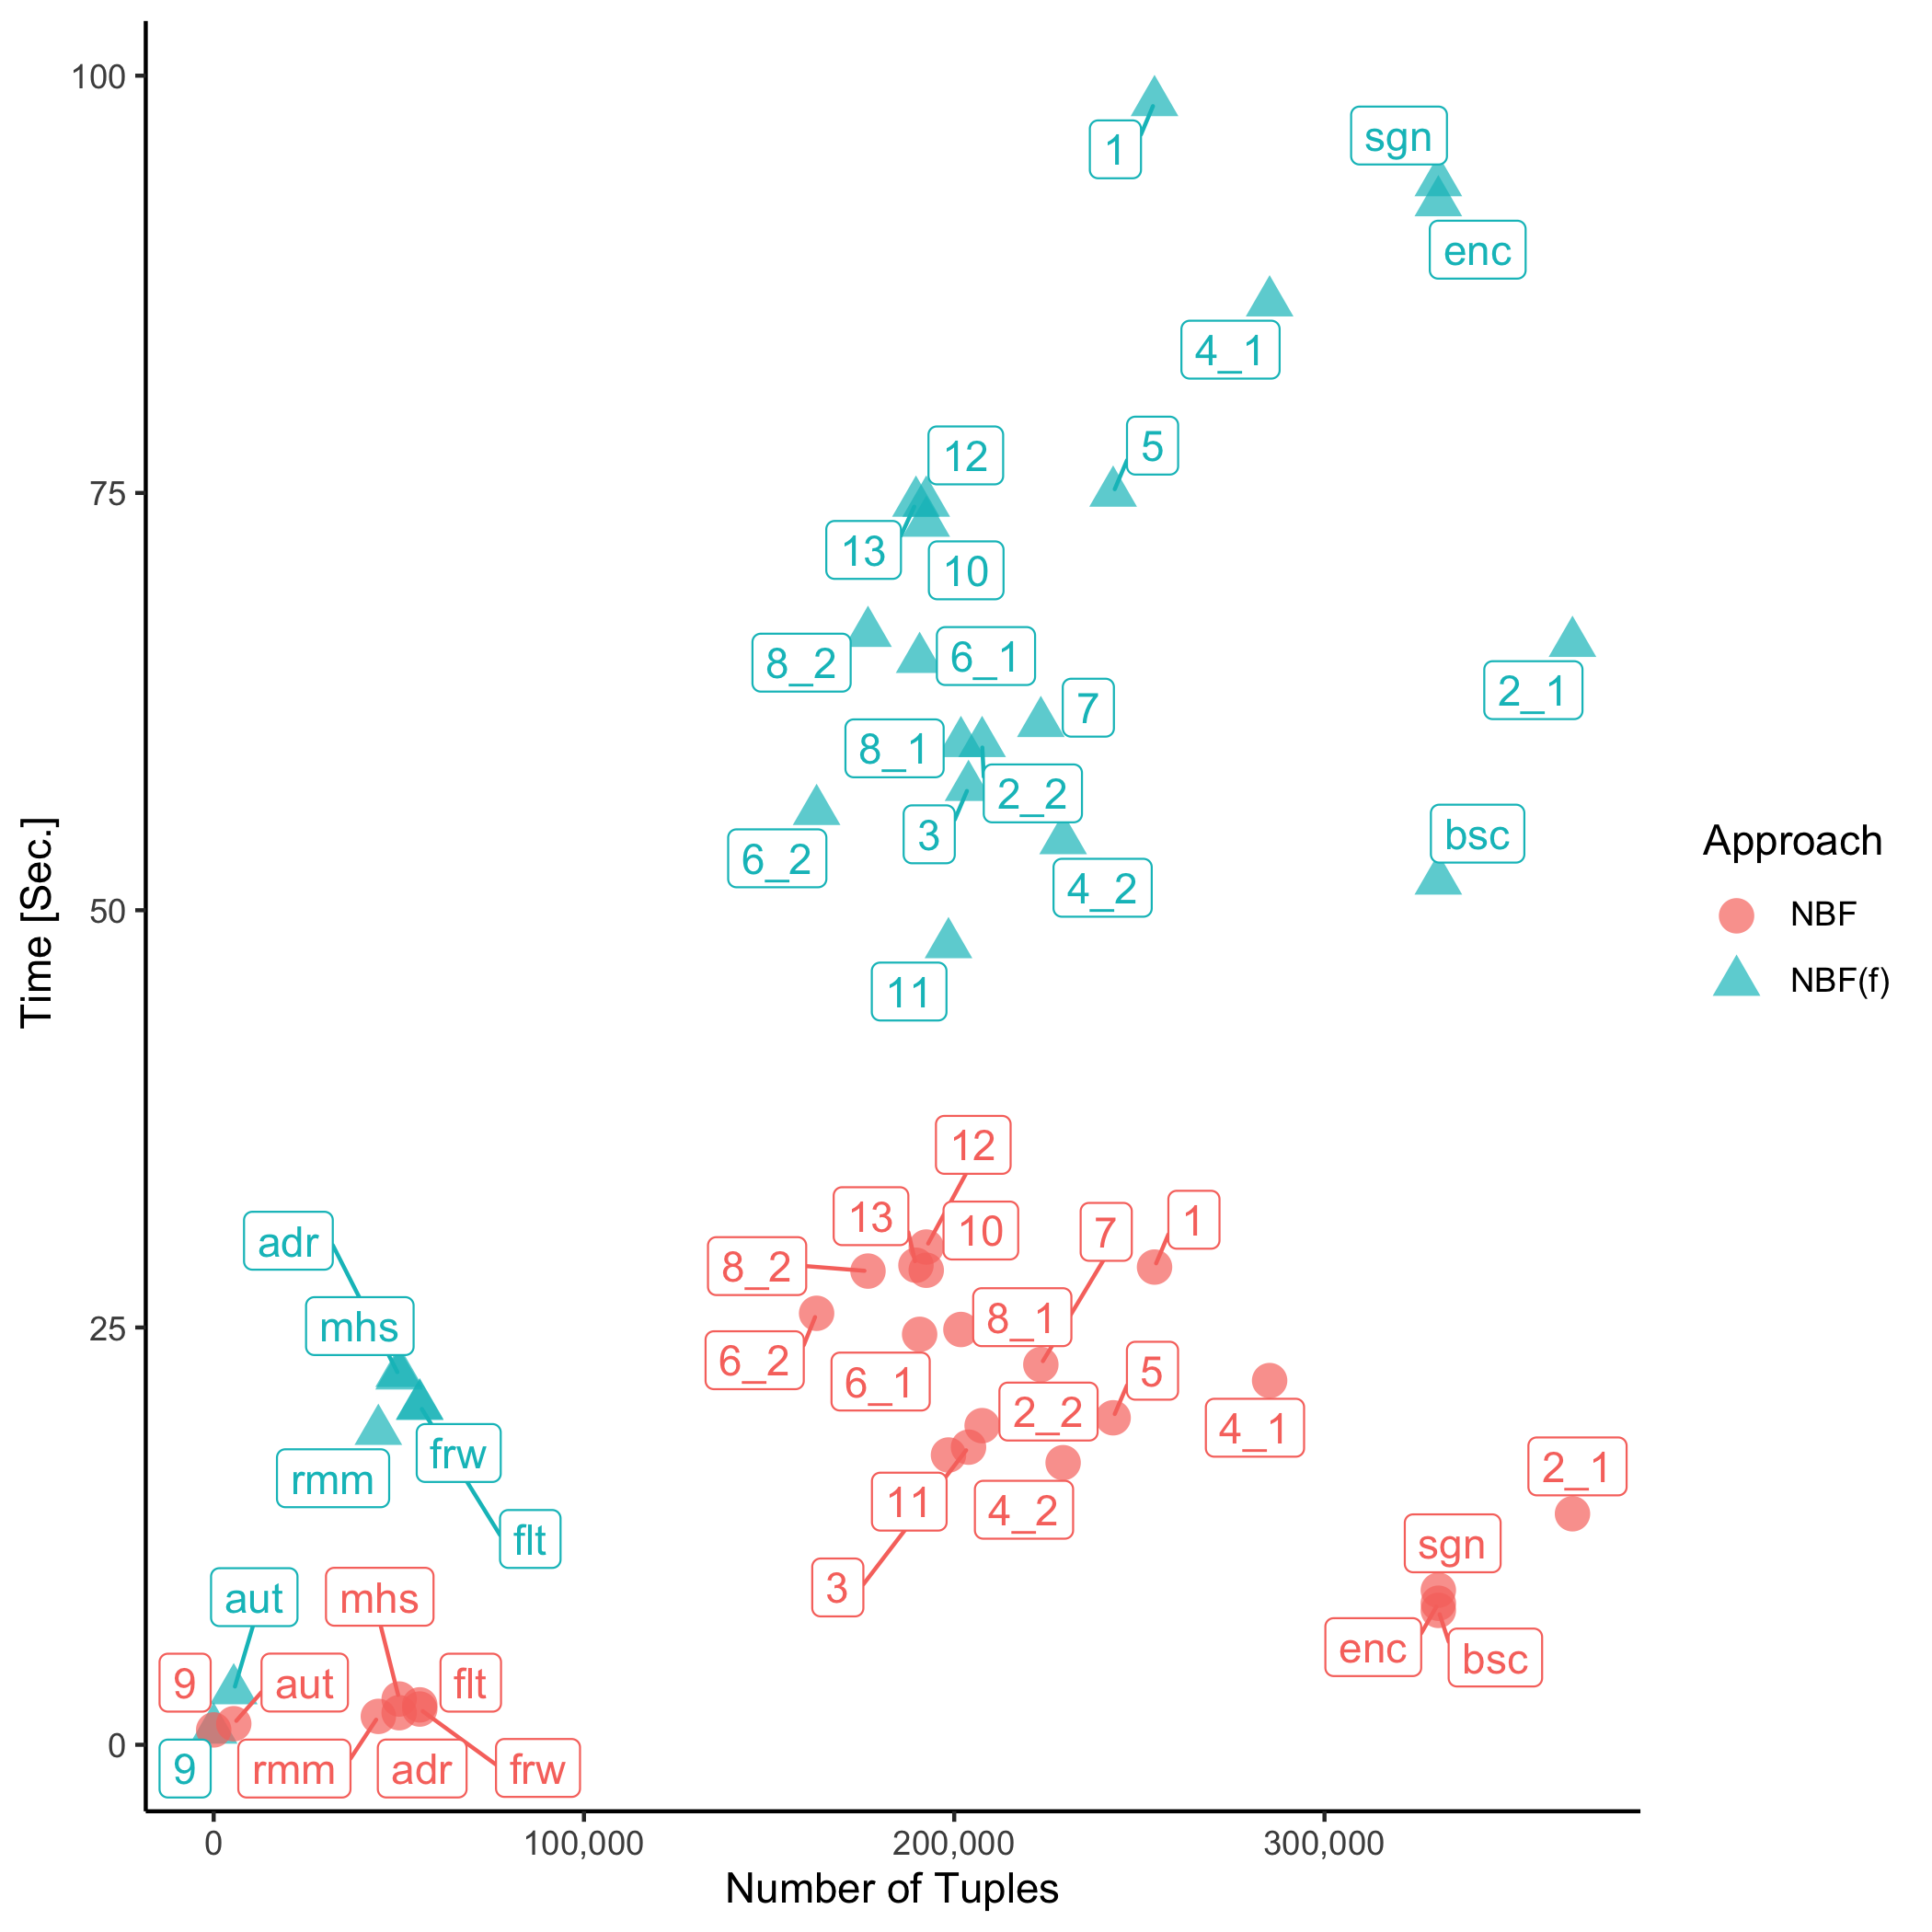
\includegraphics[scale=0.09]{figs/plots/enron-nbf-f-comp-scatter.png}
%        \caption{Lorem ipsum, lorem ipsum,Lorem ipsum, lorem ipsum,Lorem ipsum}
%    \end{subfigure}
%    \caption{Caption place holder}
%\end{figure*}


\begin{figure*}[t!]
    \centering
    \begin{subfigure}[t]{0.5\textwidth}
        \centering
        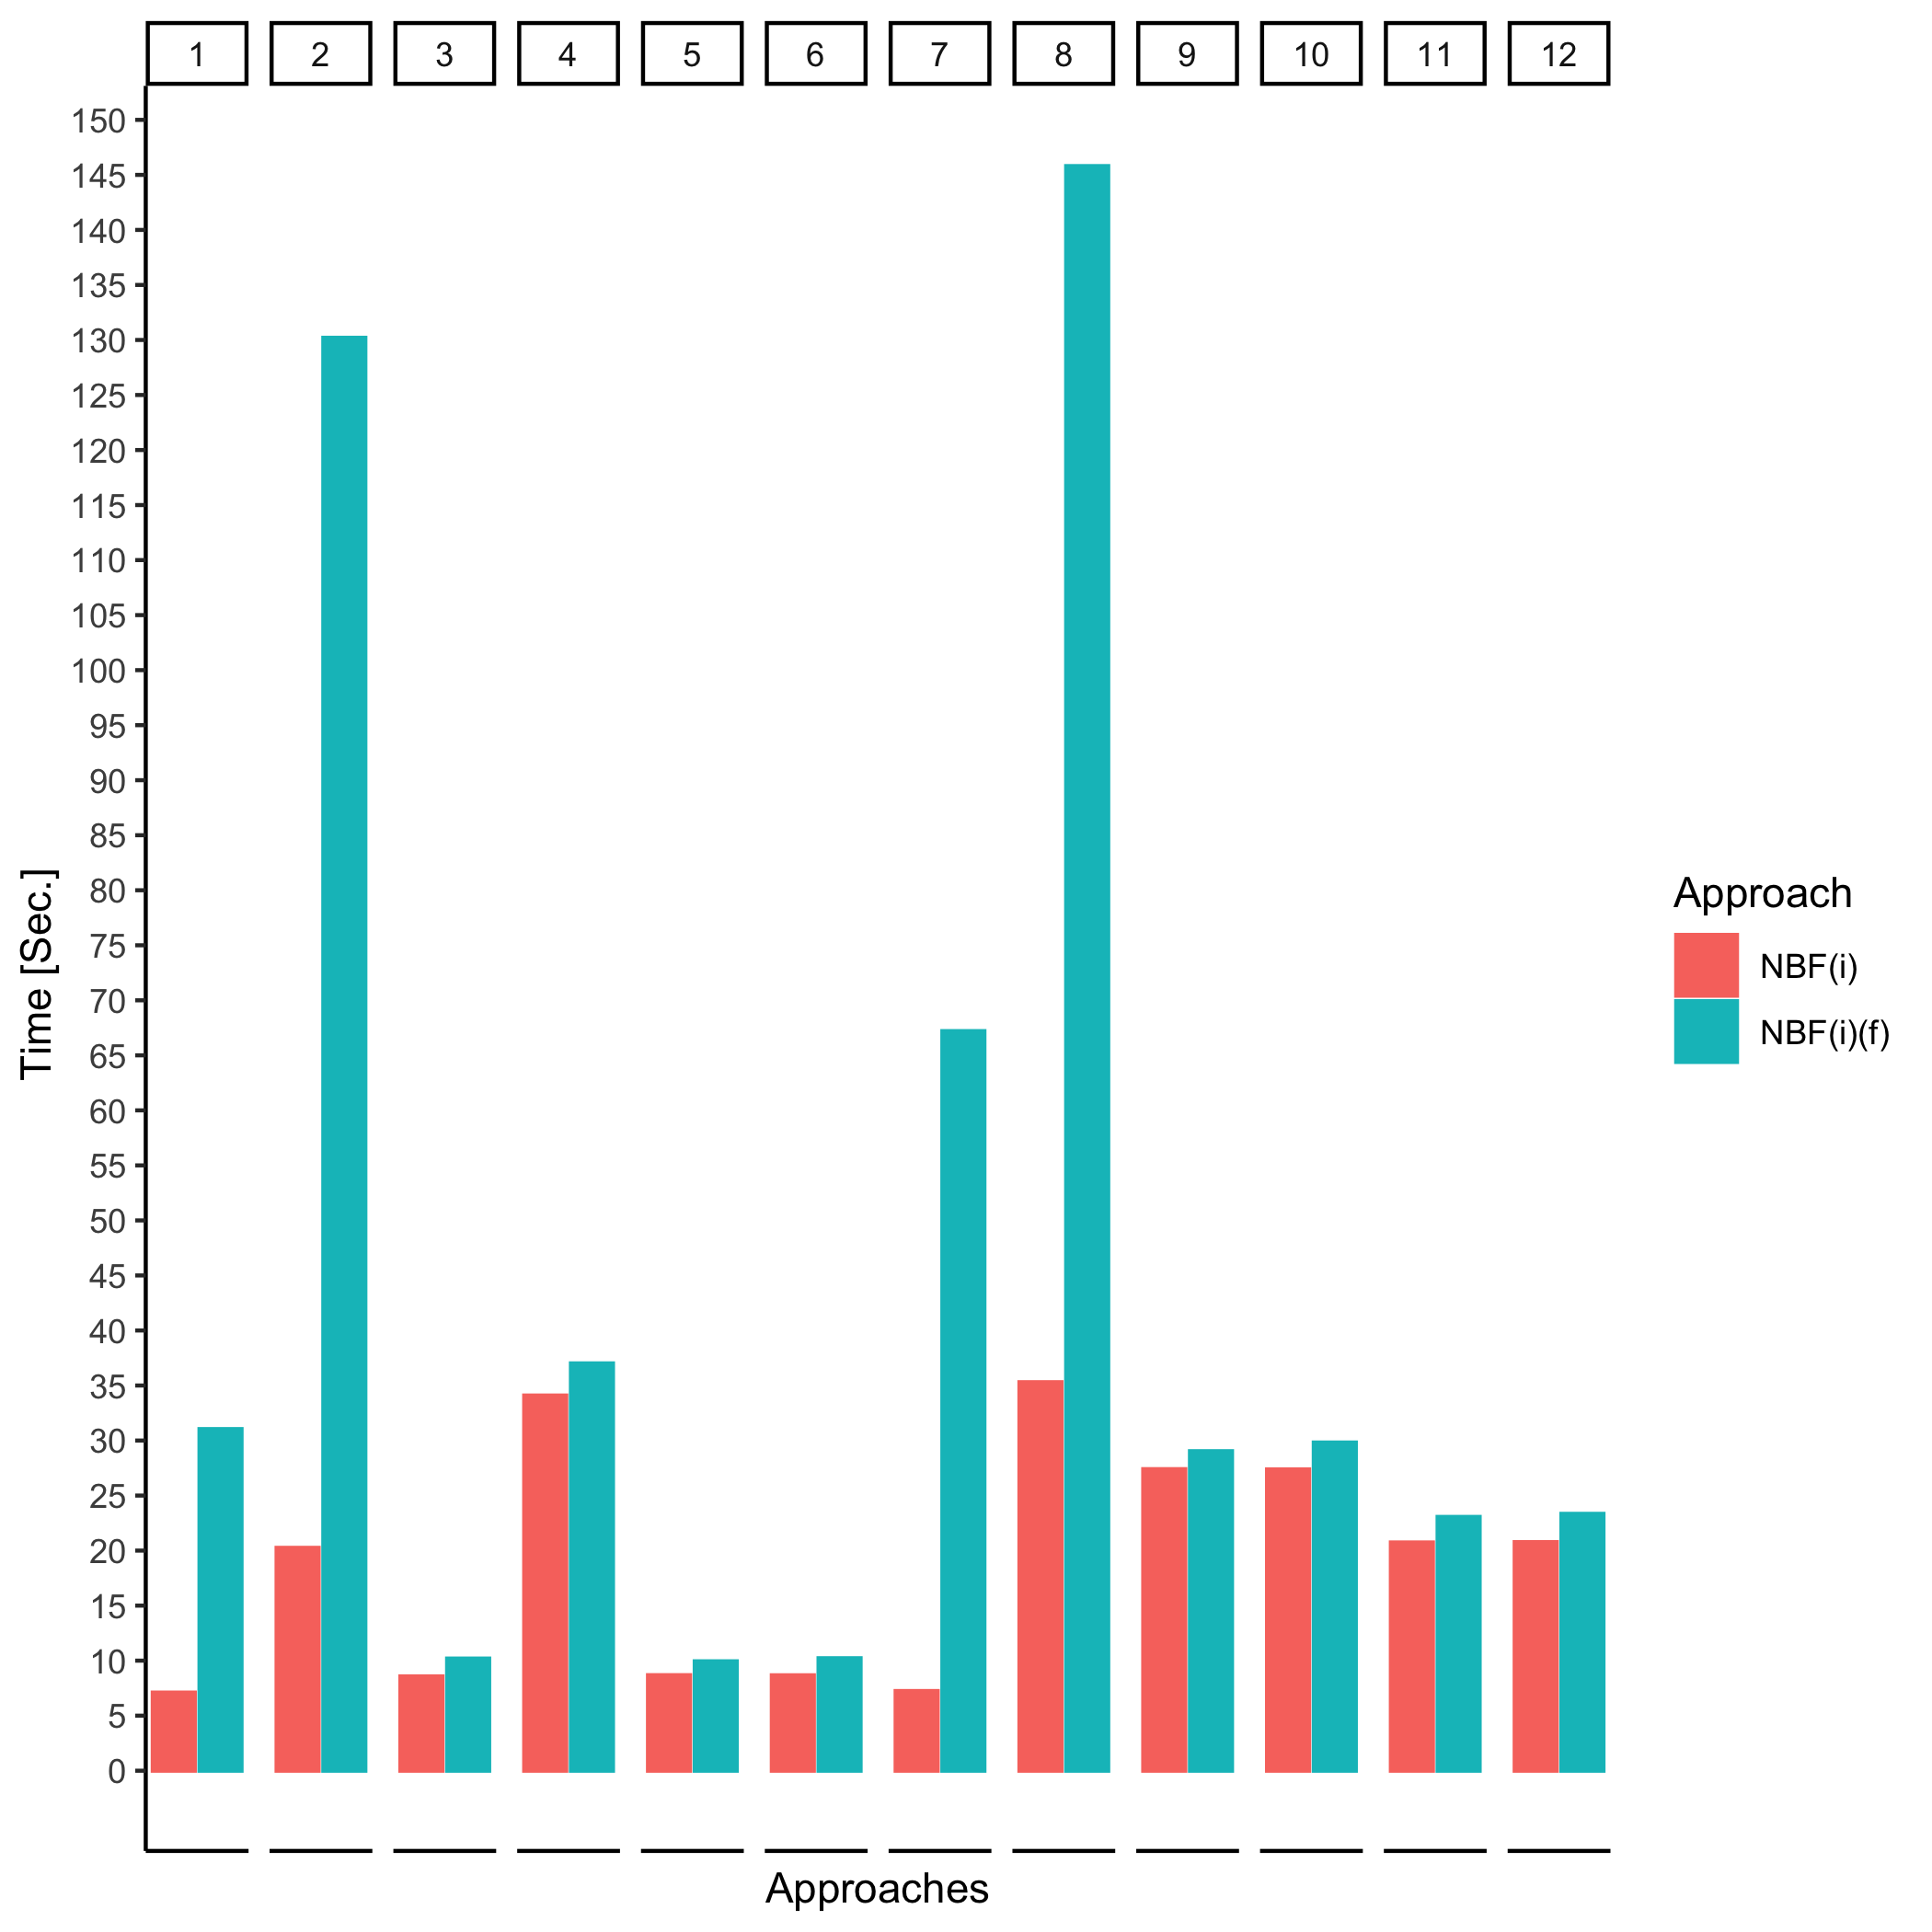
\includegraphics[scale=0.09]{figs/plots/emp-nbfi-comp-f.png}
        \caption[The \nbfi\ approach versus \nbfif]{The \nbfi\ approach versus \nbfif.}
    \end{subfigure}%
    ~ 
    \begin{subfigure}[t]{0.5\textwidth}
        \centering
        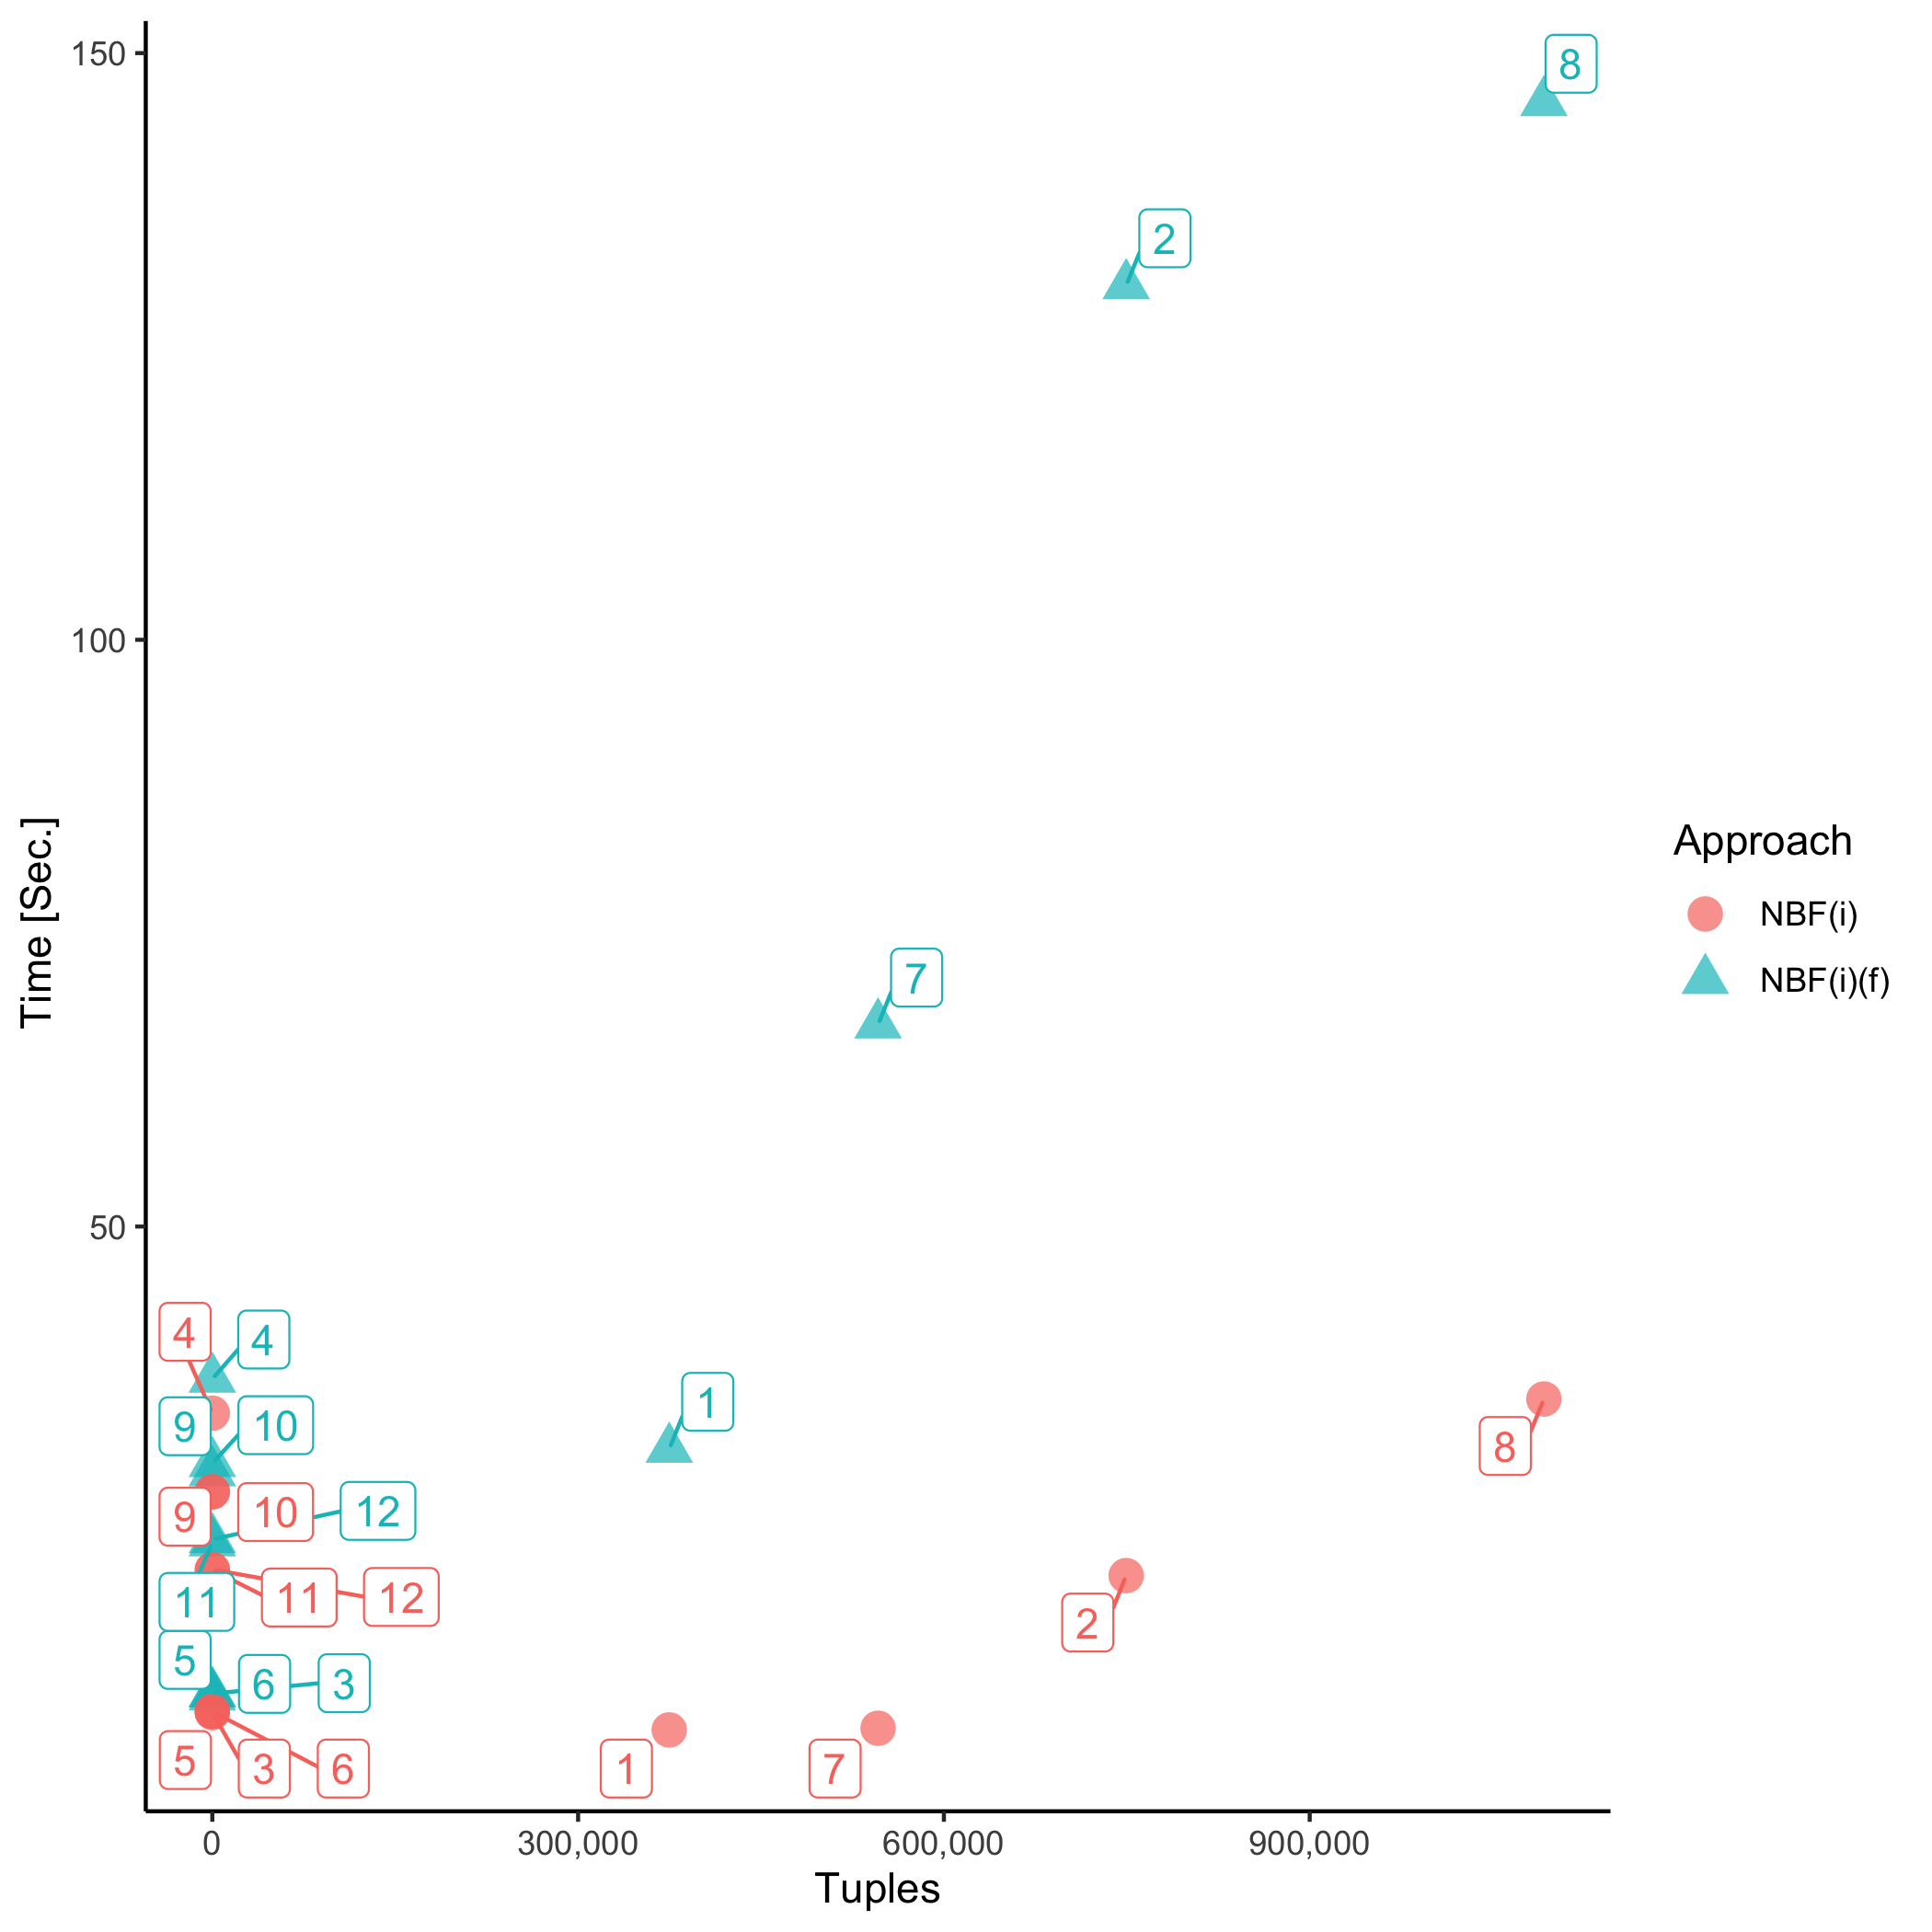
\includegraphics[scale=0.09]{figs/plots/emp-nbfi-f-comp-scatter.png}
        \caption[The \nbfi\ approach versus \nbfif\ as the number of returned tuples increases]{The \nbfi\ approach versus \nbfif\ as the number of returned tuples increases.}
        \label{fig:emp-nbfi-tuple}
    \end{subfigure}\\[1ex]
    \begin{subfigure}[t]{0.5\textwidth}
        \centering
        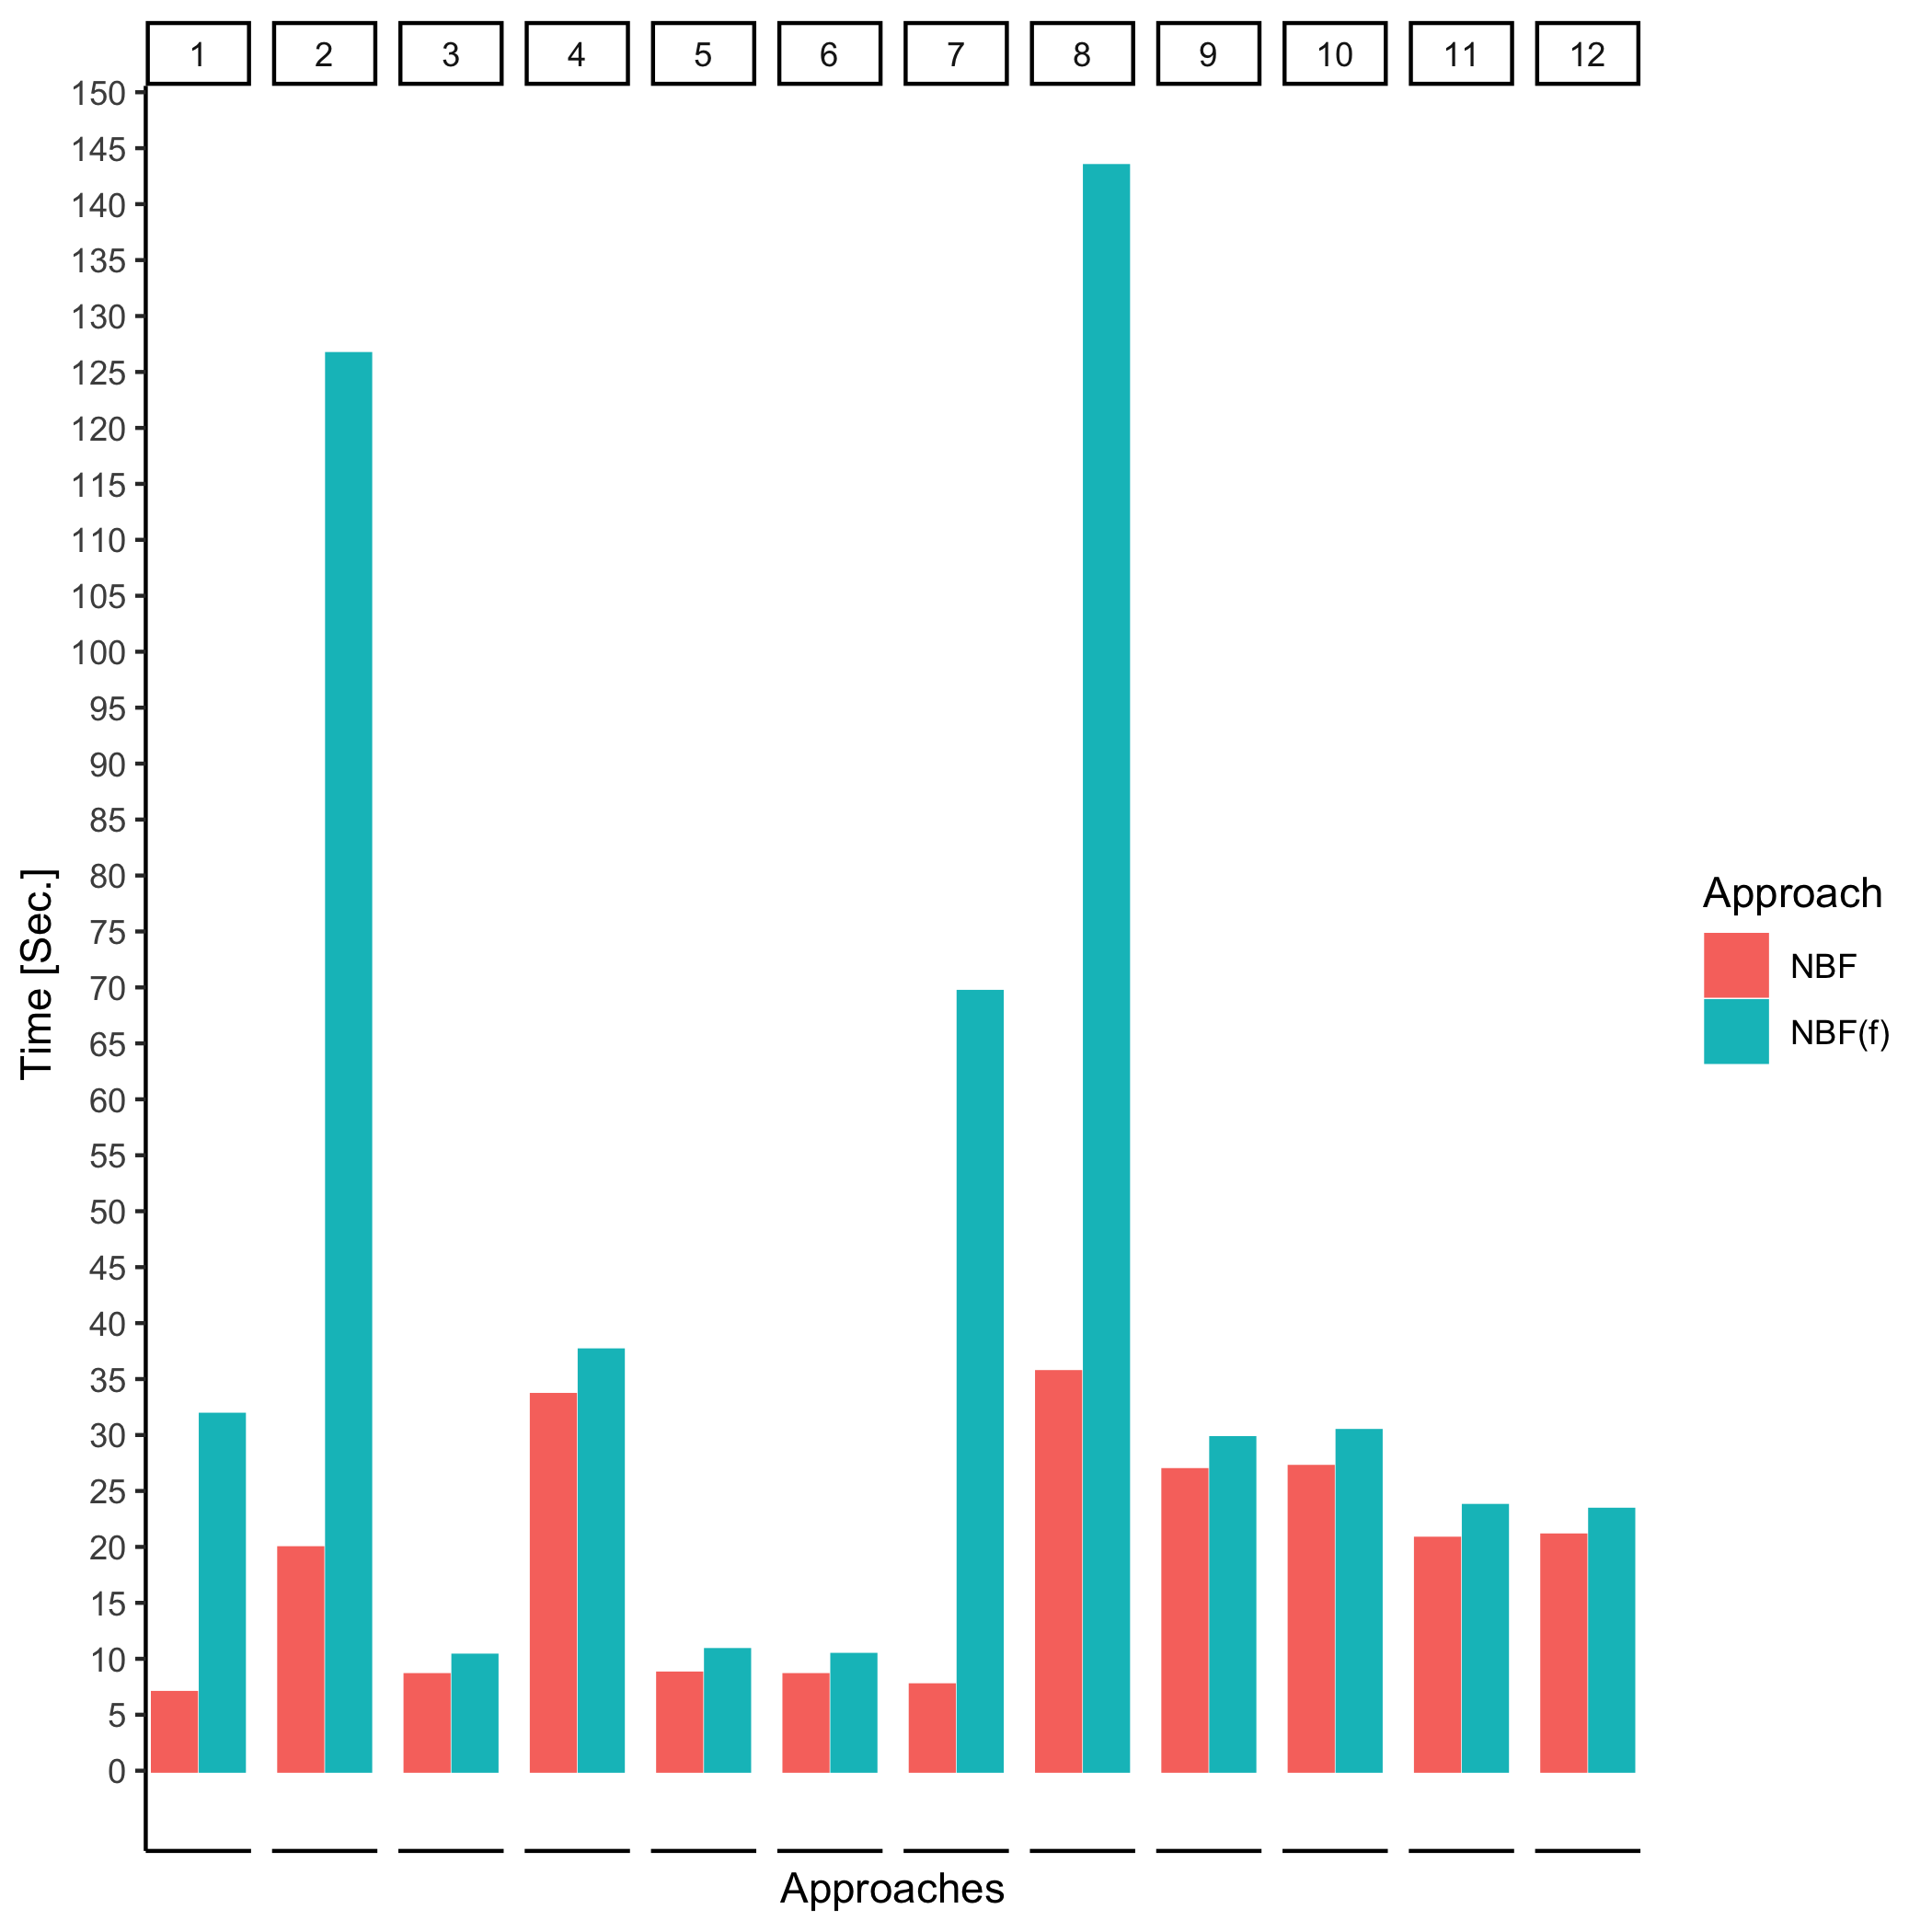
\includegraphics[scale=0.09]{figs/plots/emp-nbf-comp-f.png}
        \caption[The \nbf\ approach versus \nbff]{The \nbf\ approach versus \nbff.}
    \end{subfigure}%
    ~ 
    \begin{subfigure}[t]{0.5\textwidth}
        \centering
        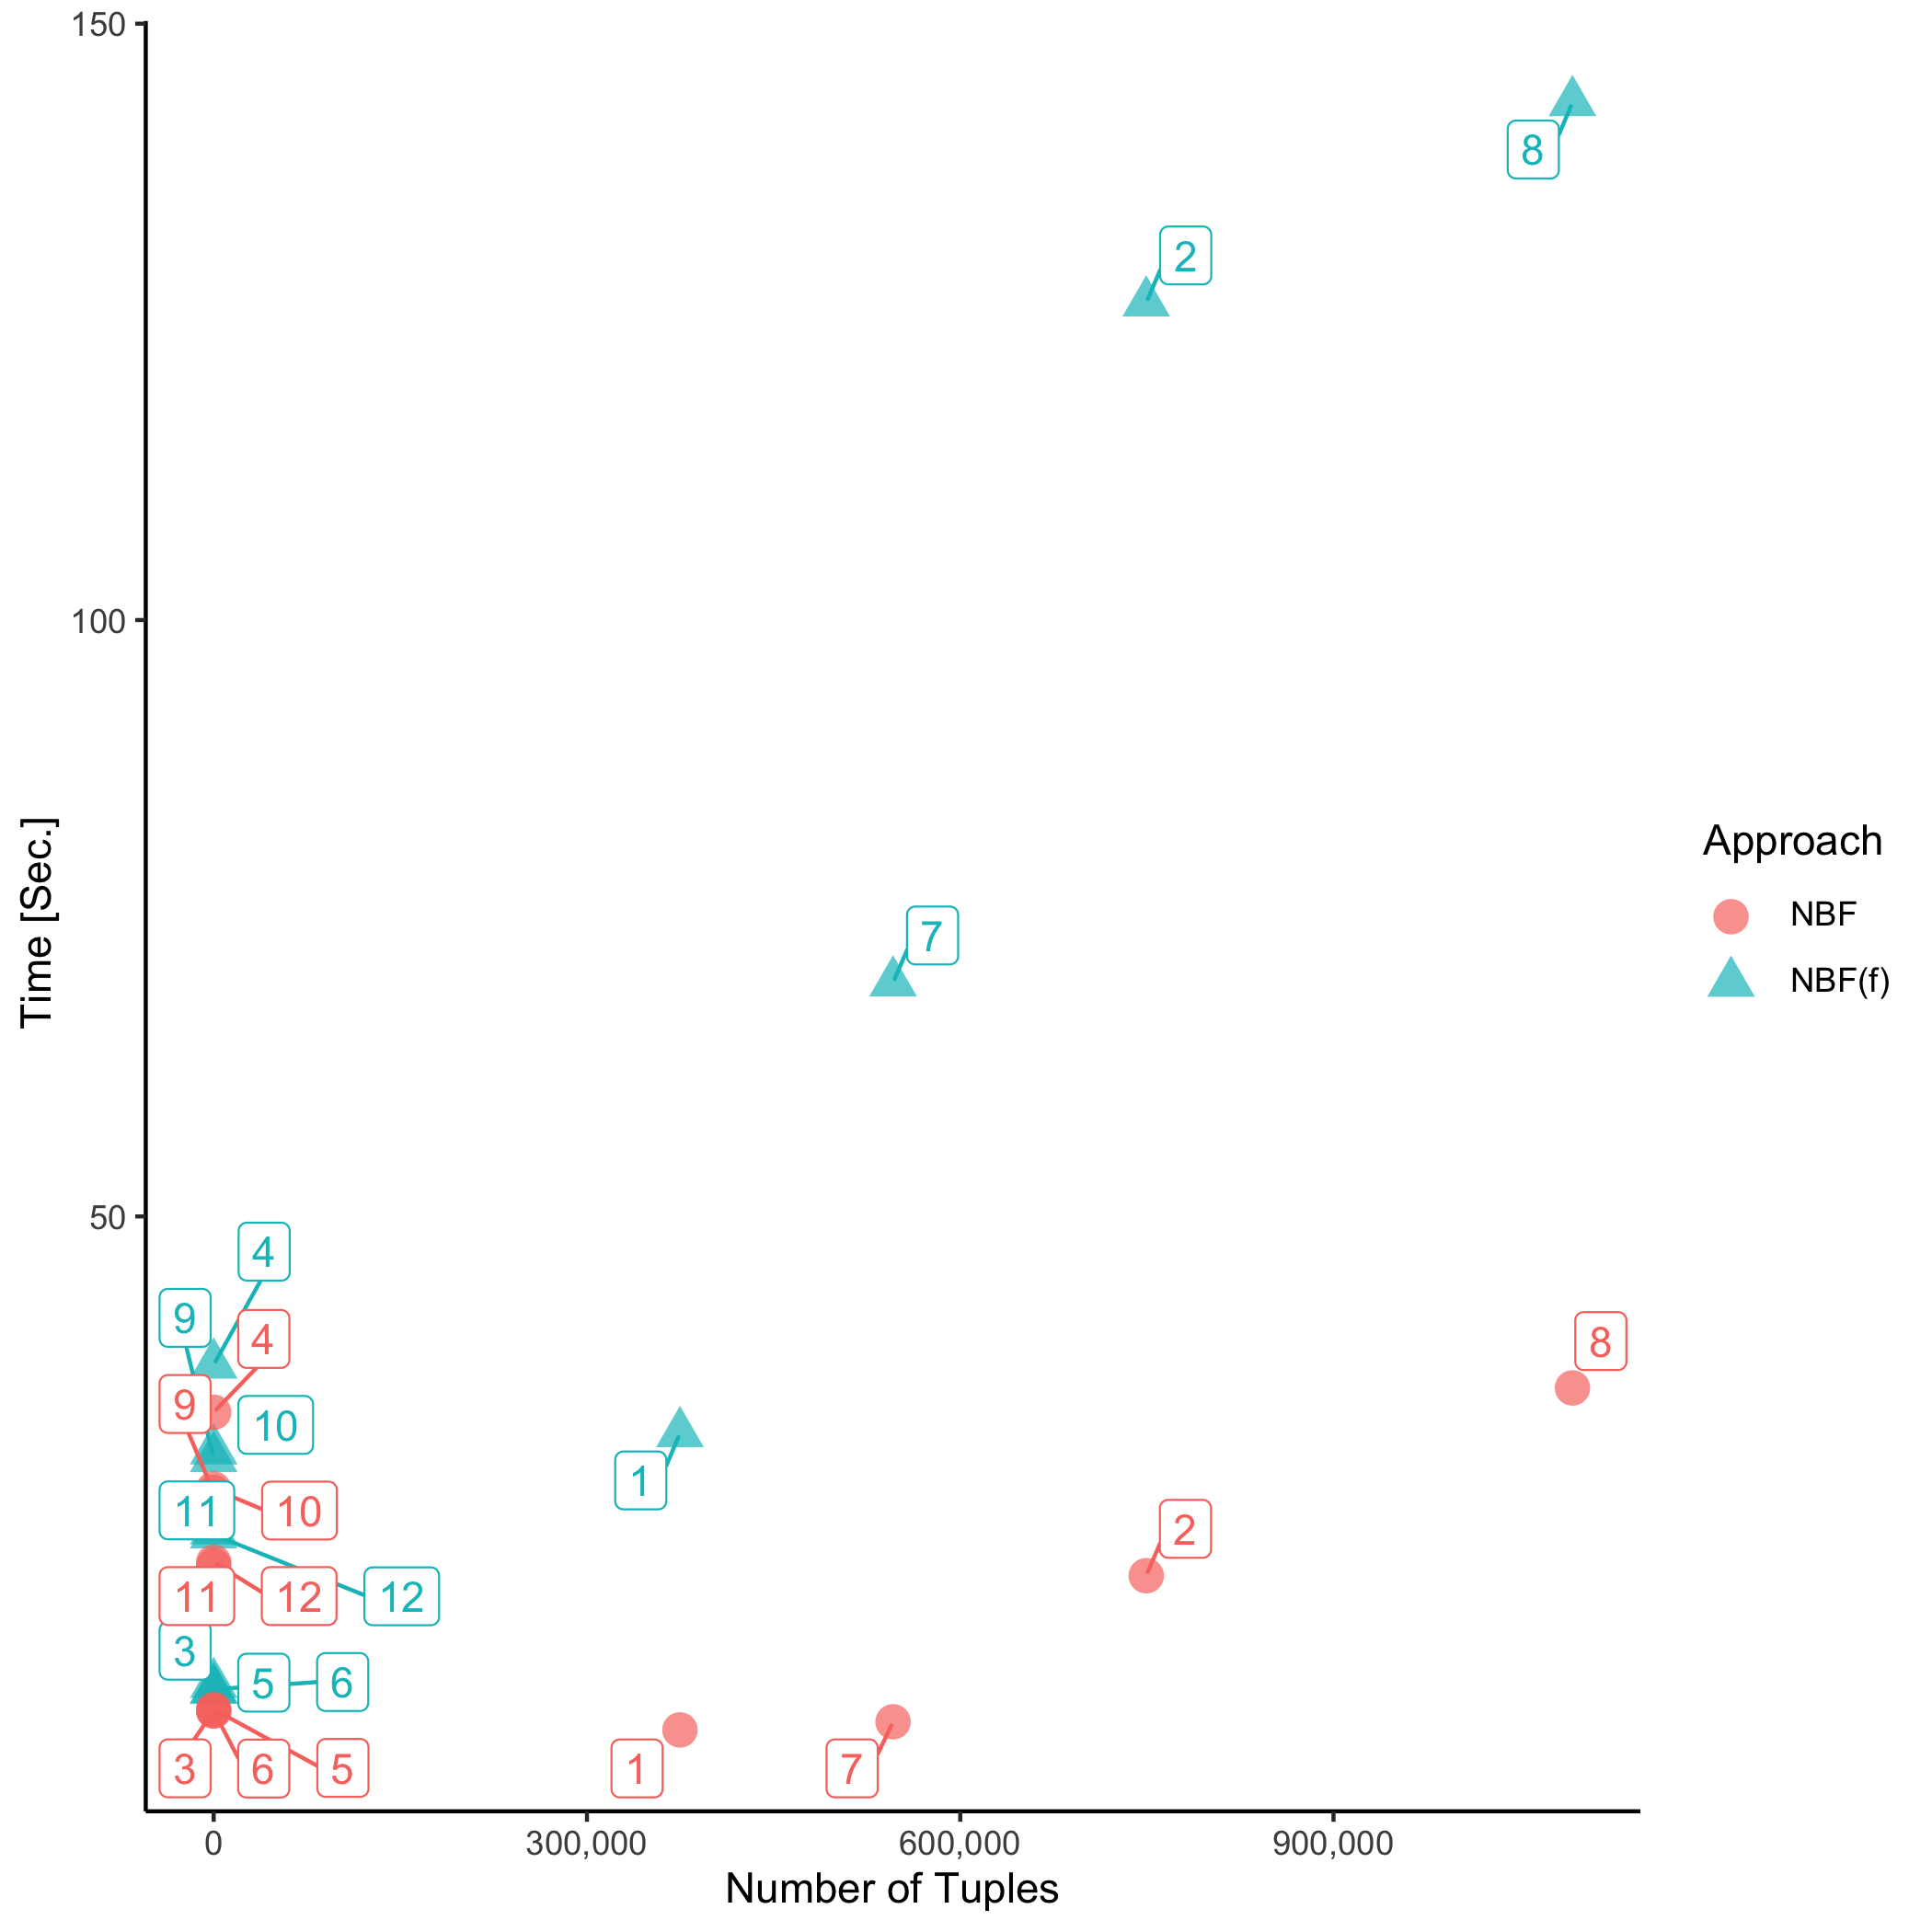
\includegraphics[scale=0.09]{figs/plots/emp-nbf-f-comp-scatter.png}
        \caption[The \nbf\ approach versus \nbff\ as the number of returned tuples increases]{The \nbf\ approach versus \nbff\ as the number of returned tuples increases.}
        \label{fig:emp-nbf-tuple}
    \end{subfigure}    
    \caption[The effect of filtering out tuples with unsatisfiable presence conditions on SQL generator 
    approaches over the employee VDB]{The effect of filtering out tuples with unsatisfiable presence conditions on SQL generator 
    approaches over the employee VDB.}
    \label{fig:emp-nbfs-filter}
\end{figure*}

%\begin{figure*}[t!]
%    \centering
%    \begin{subfigure}[t]{0.5\textwidth}
%        \centering
%        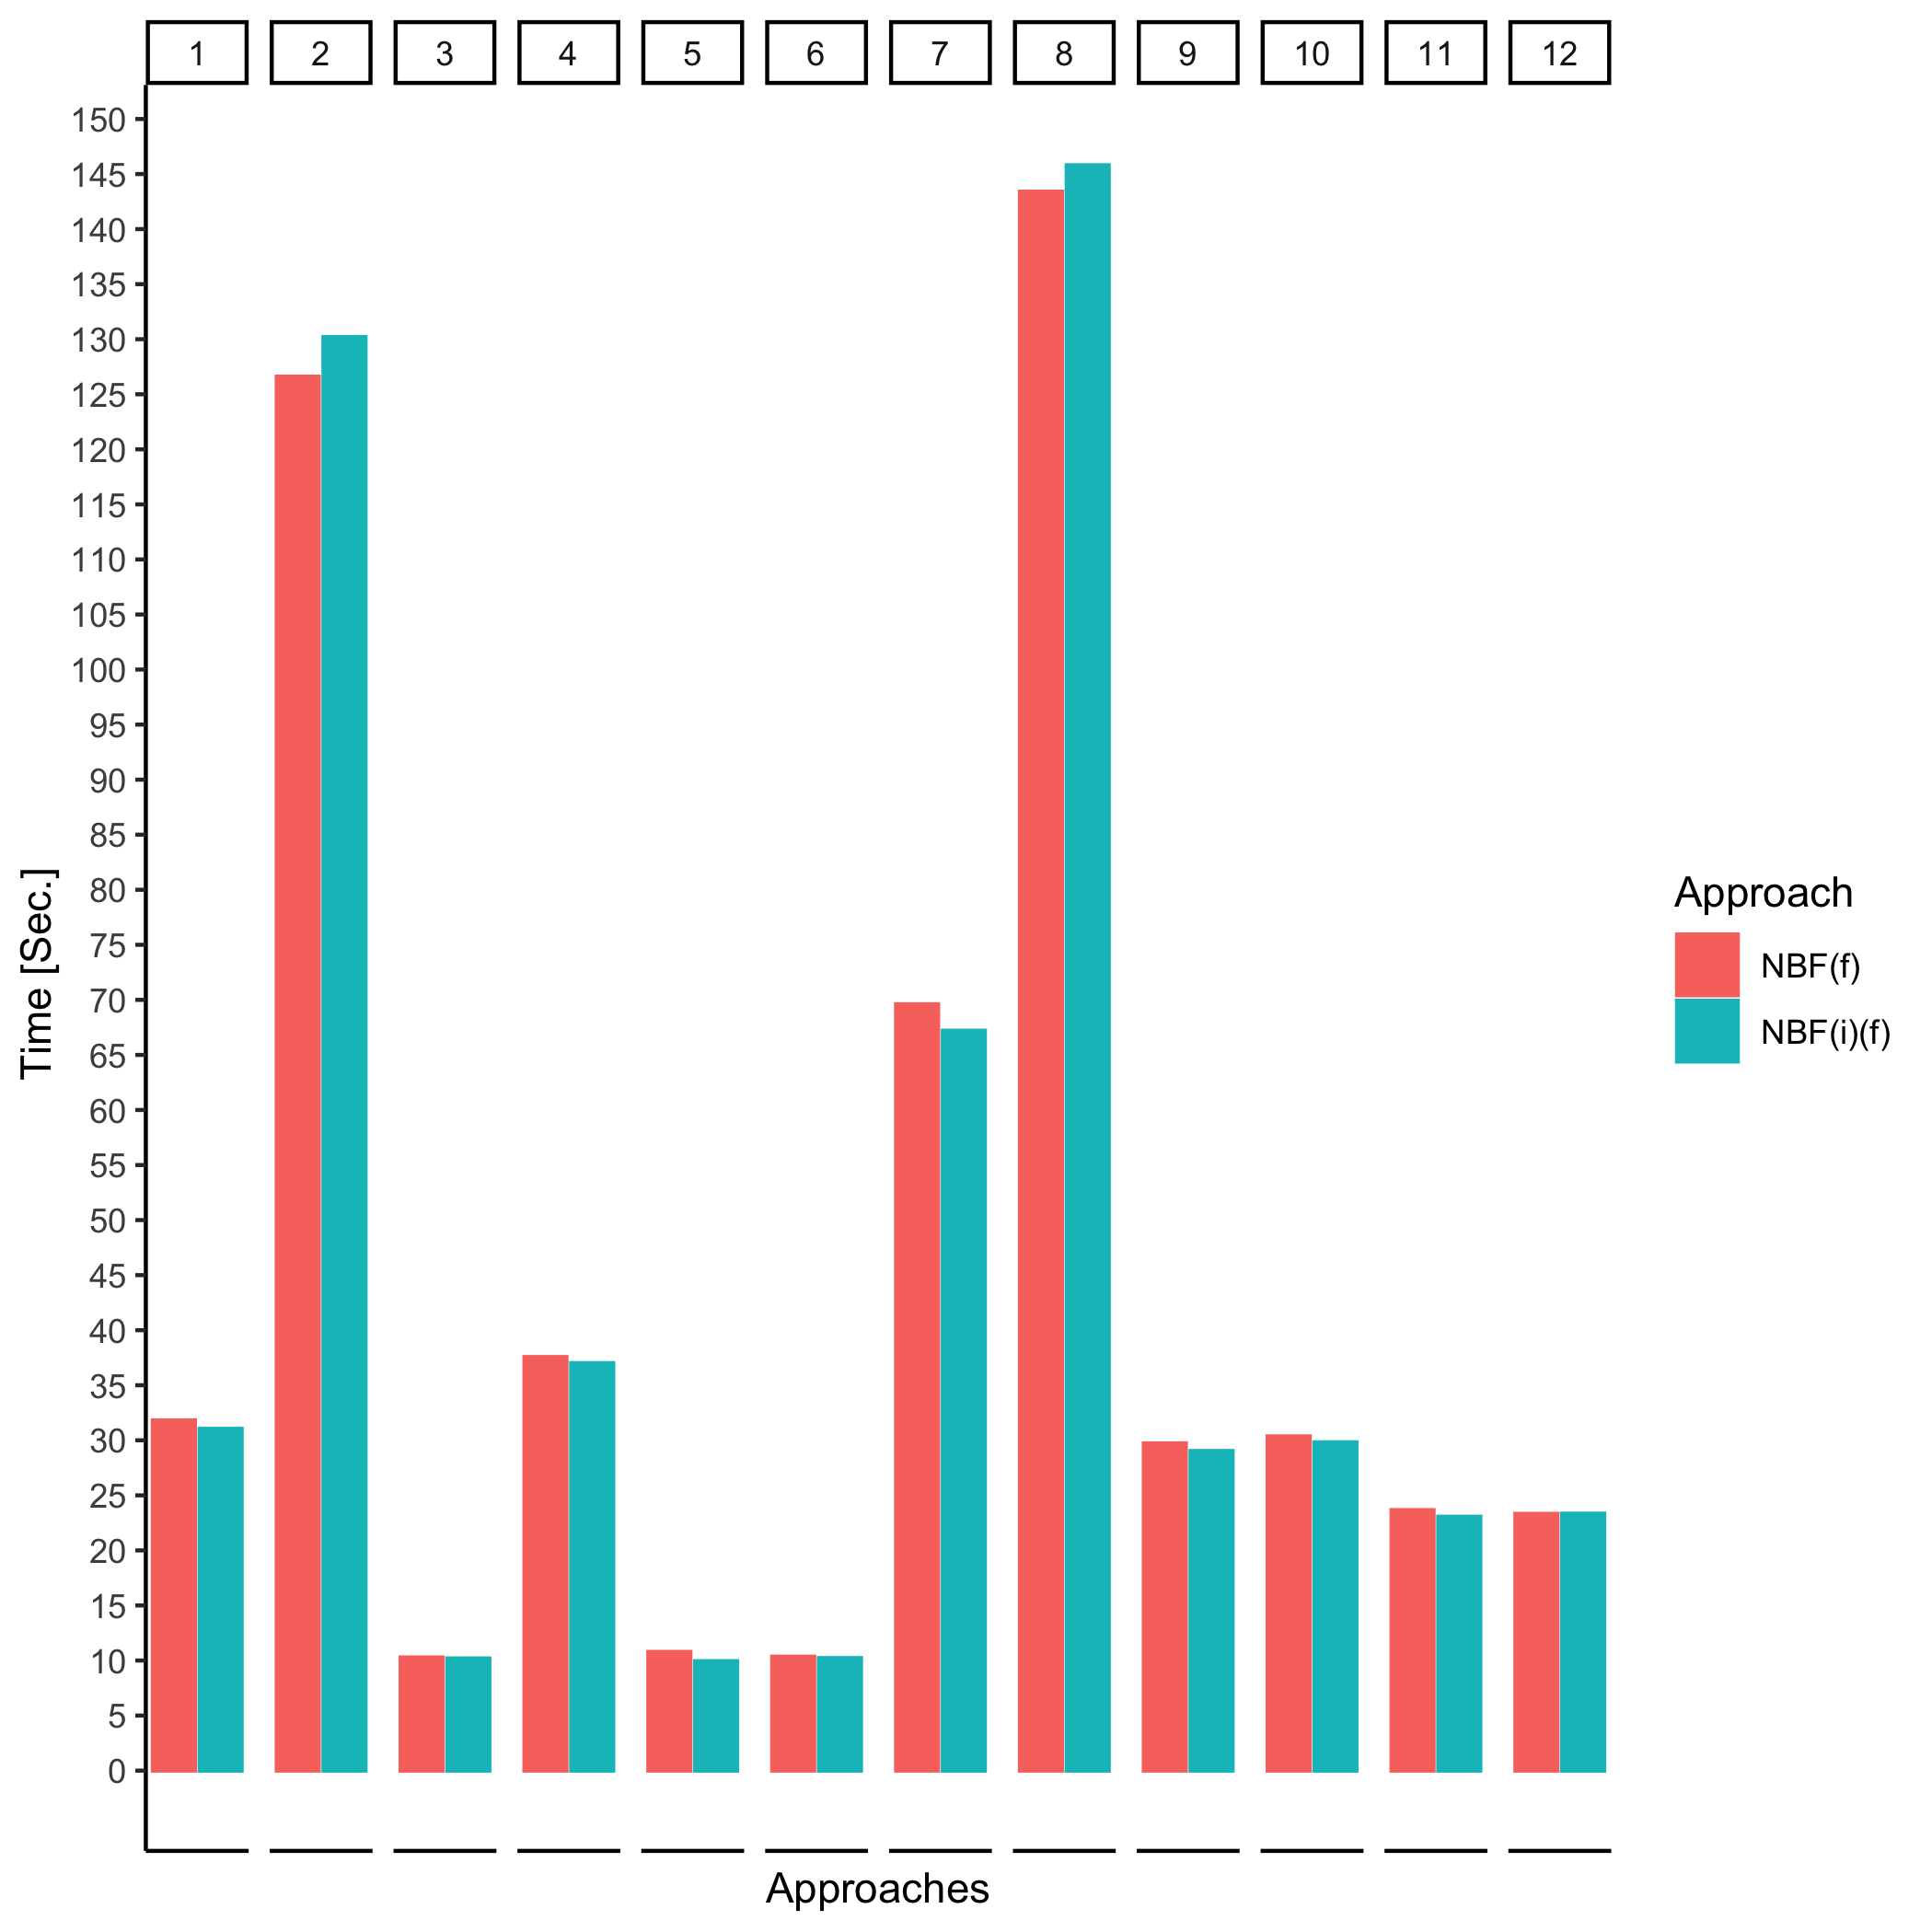
\includegraphics[scale=0.09]{figs/plots/emp-nbf-f.png}
%        \caption{Lorem ipsum}
%    \end{subfigure}%
%    ~ 
%    \begin{subfigure}[t]{0.5\textwidth}
%        \centering
%        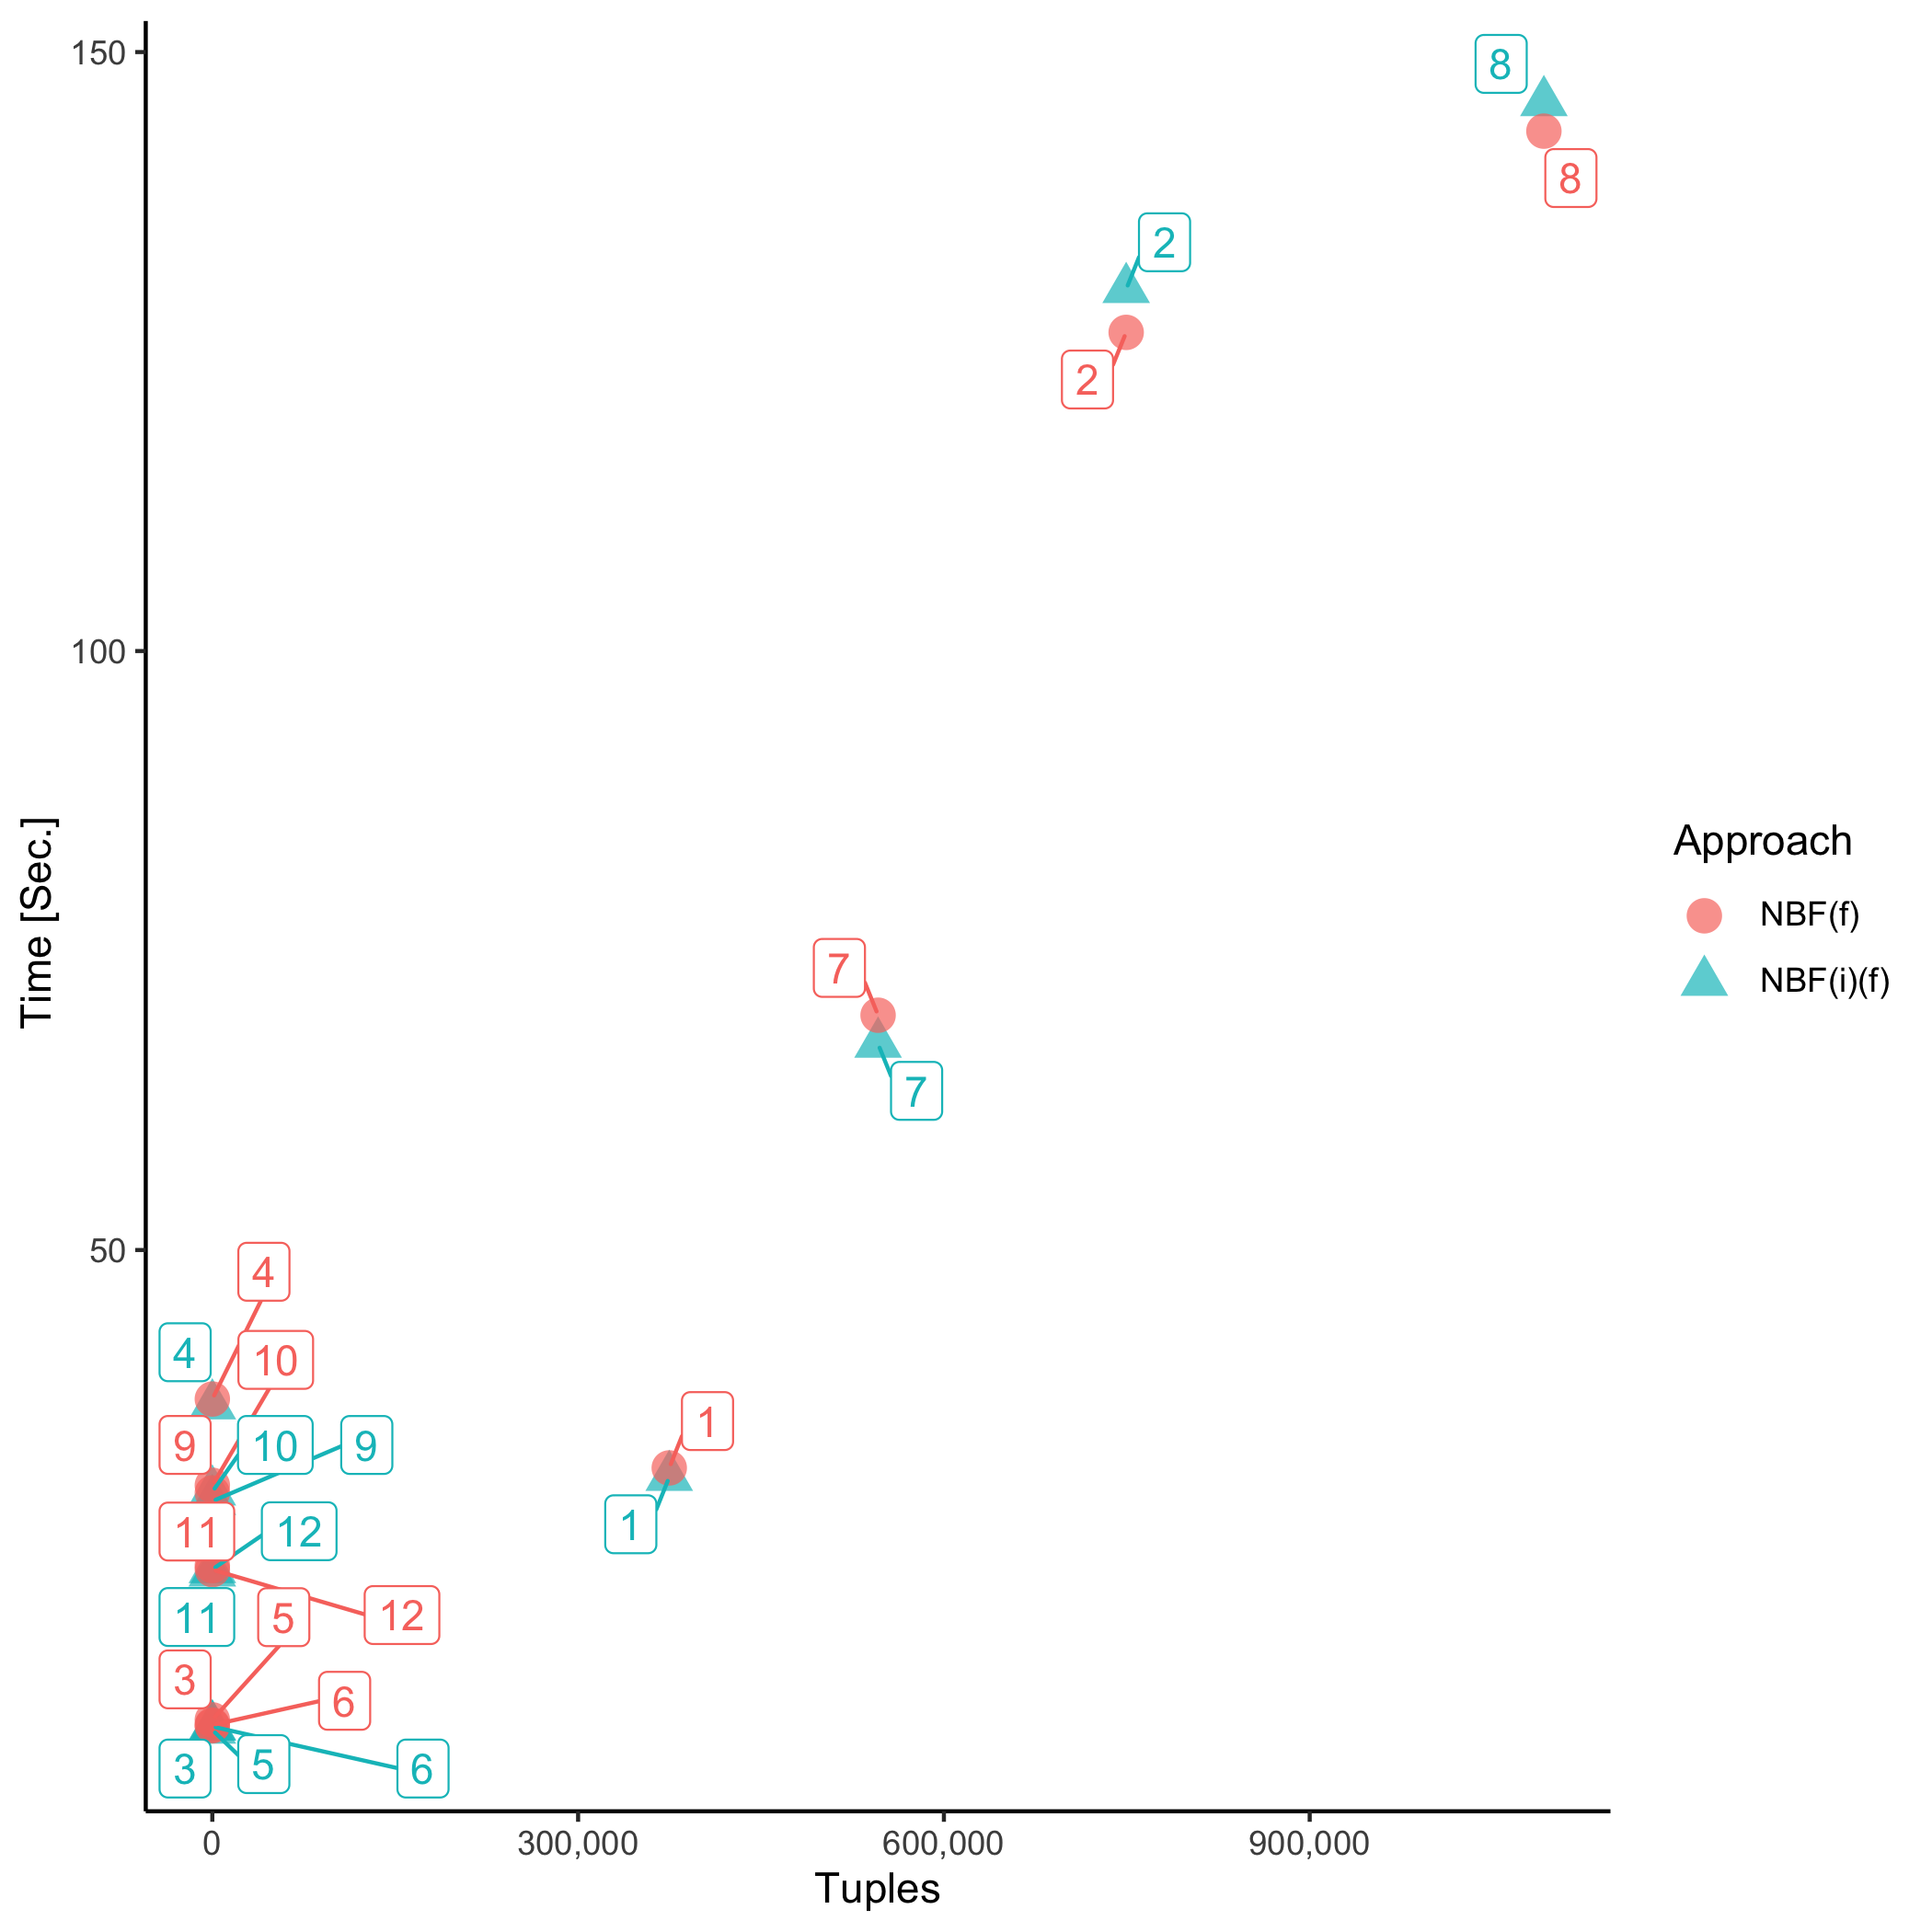
\includegraphics[scale=0.09]{figs/plots/emp-nbf-f-scatter.png}
%        \caption{Lorem ipsum, lorem ipsum,Lorem ipsum, lorem ipsum,Lorem ipsum}
%    \end{subfigure}
%    \caption{Caption place holder}
%\end{figure*}

%\begin{figure*}[t!]
%    \centering
%    \begin{subfigure}[t]{0.5\textwidth}
%        \centering
%        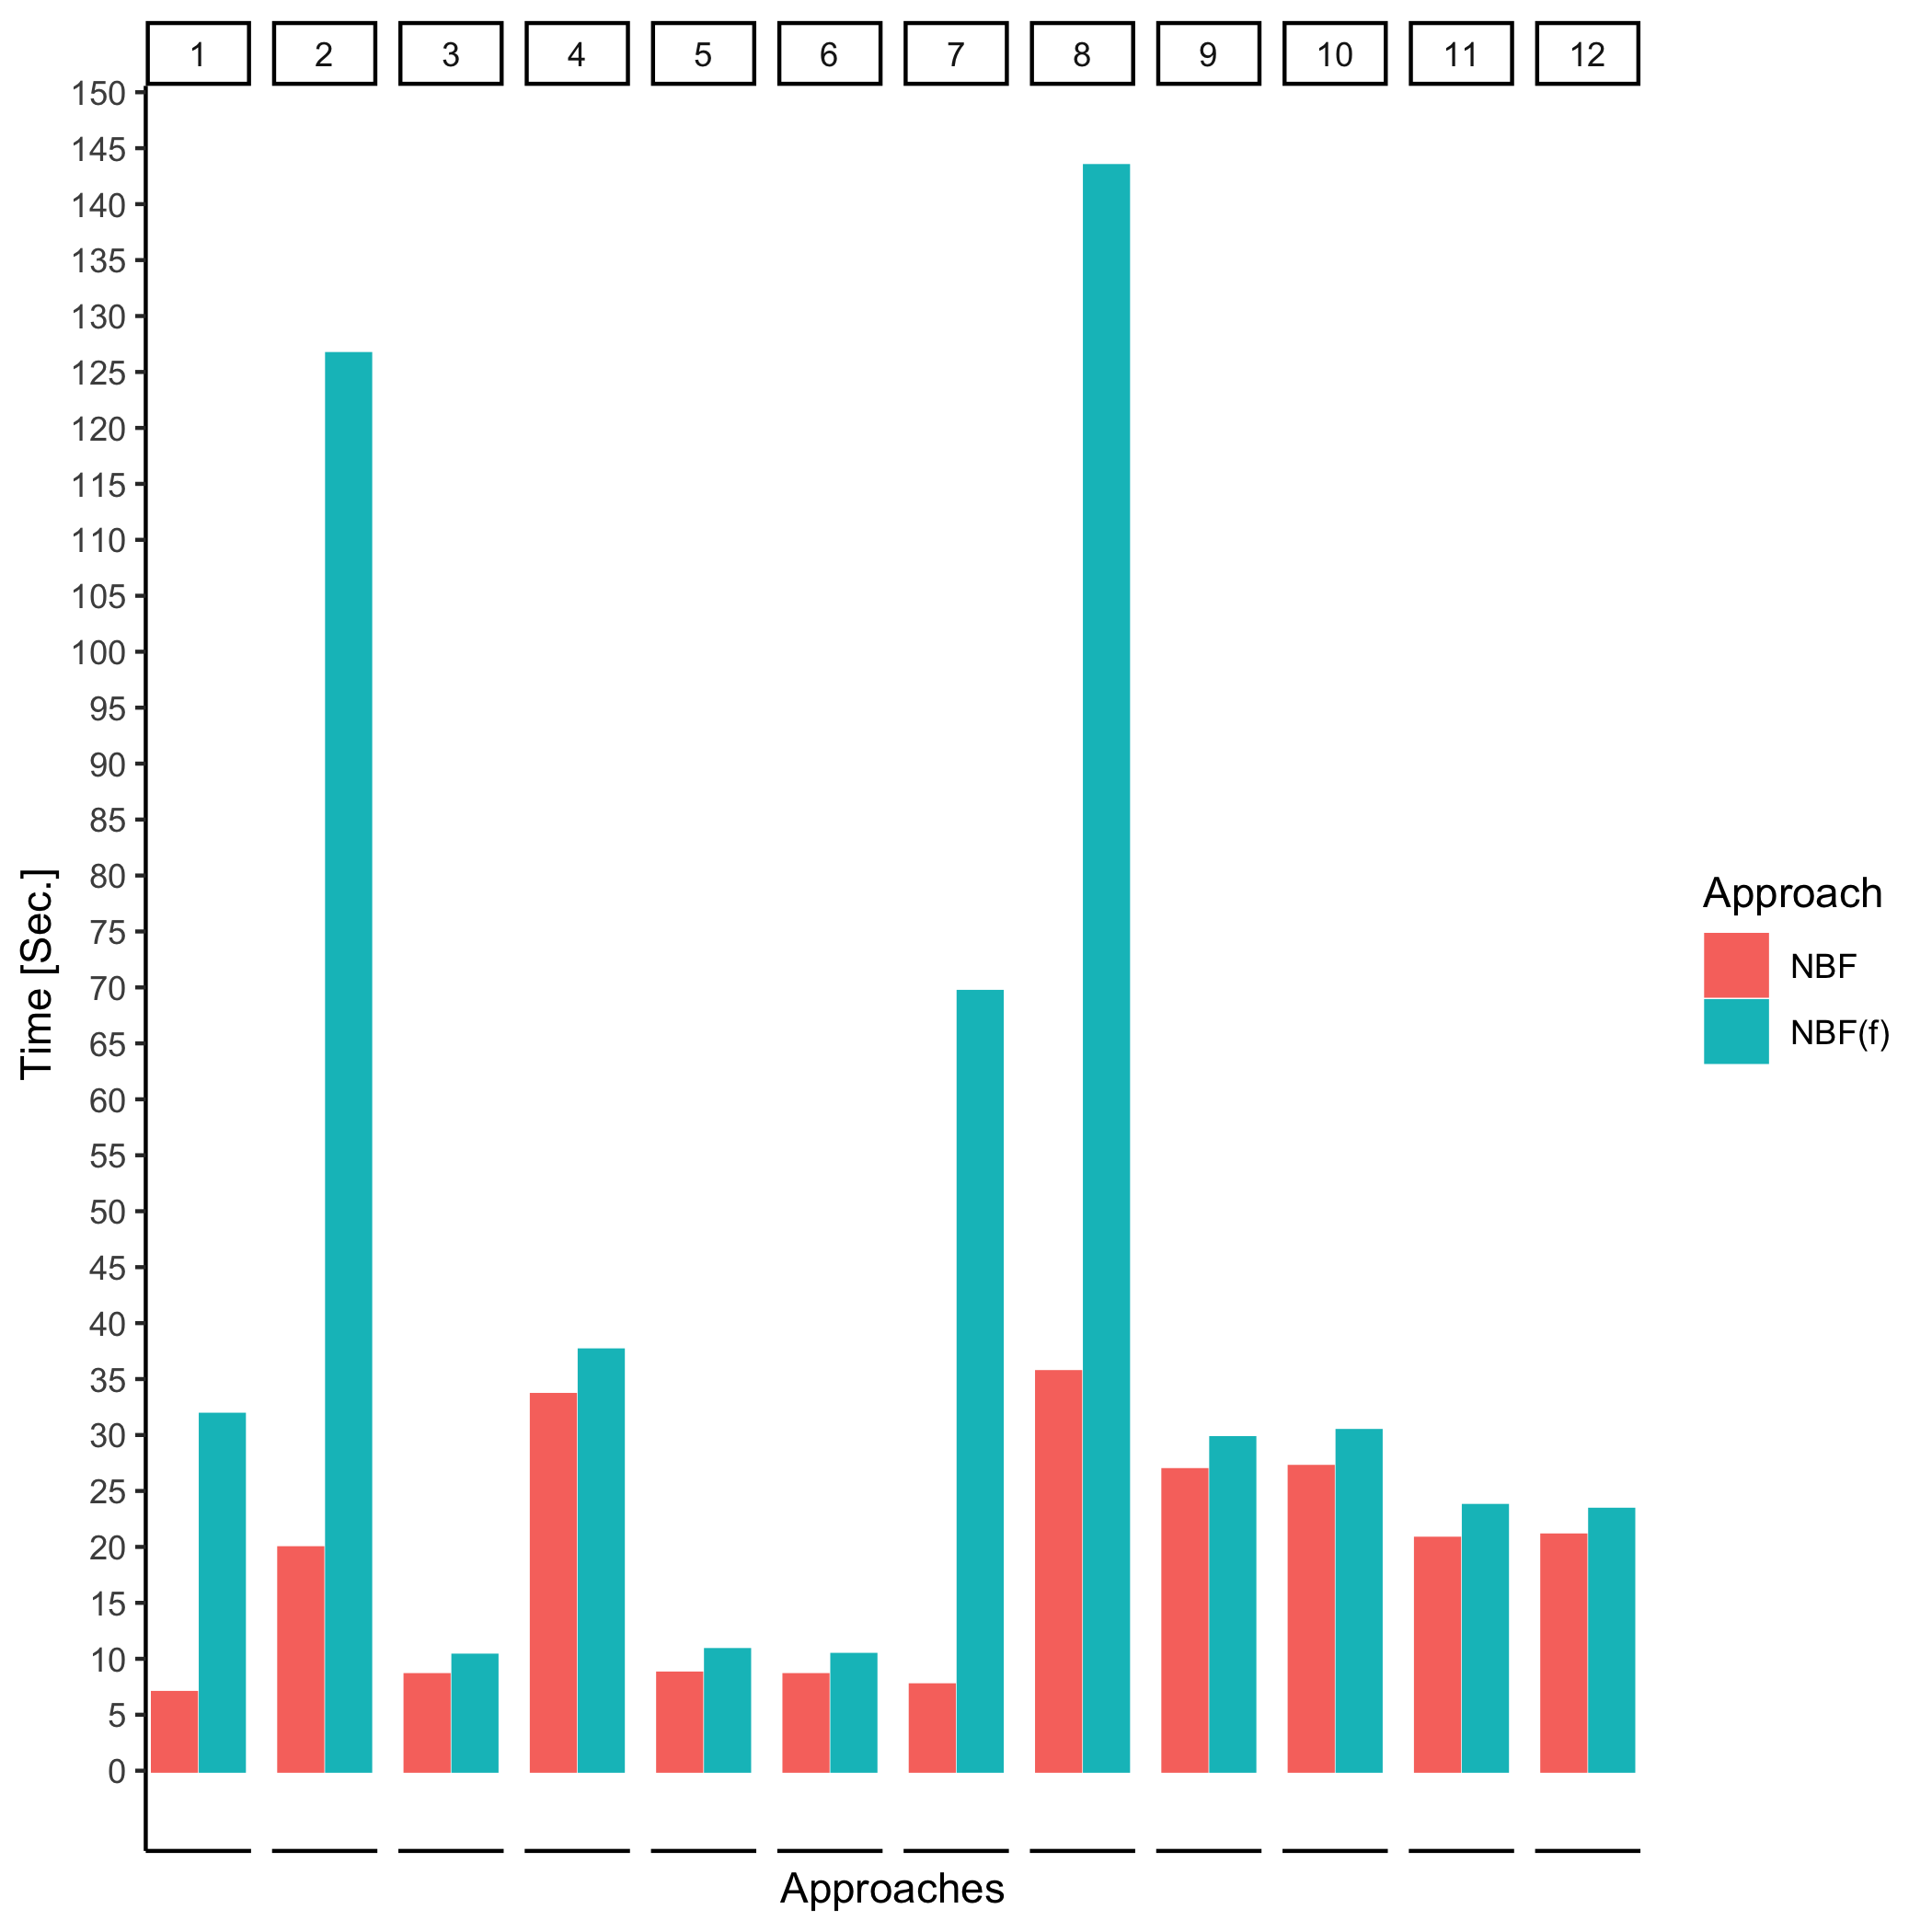
\includegraphics[scale=0.09]{figs/plots/emp-nbf-comp-f.png}
%        \caption{Lorem ipsum}
%    \end{subfigure}%
%    ~ 
%    \begin{subfigure}[t]{0.5\textwidth}
%        \centering
%        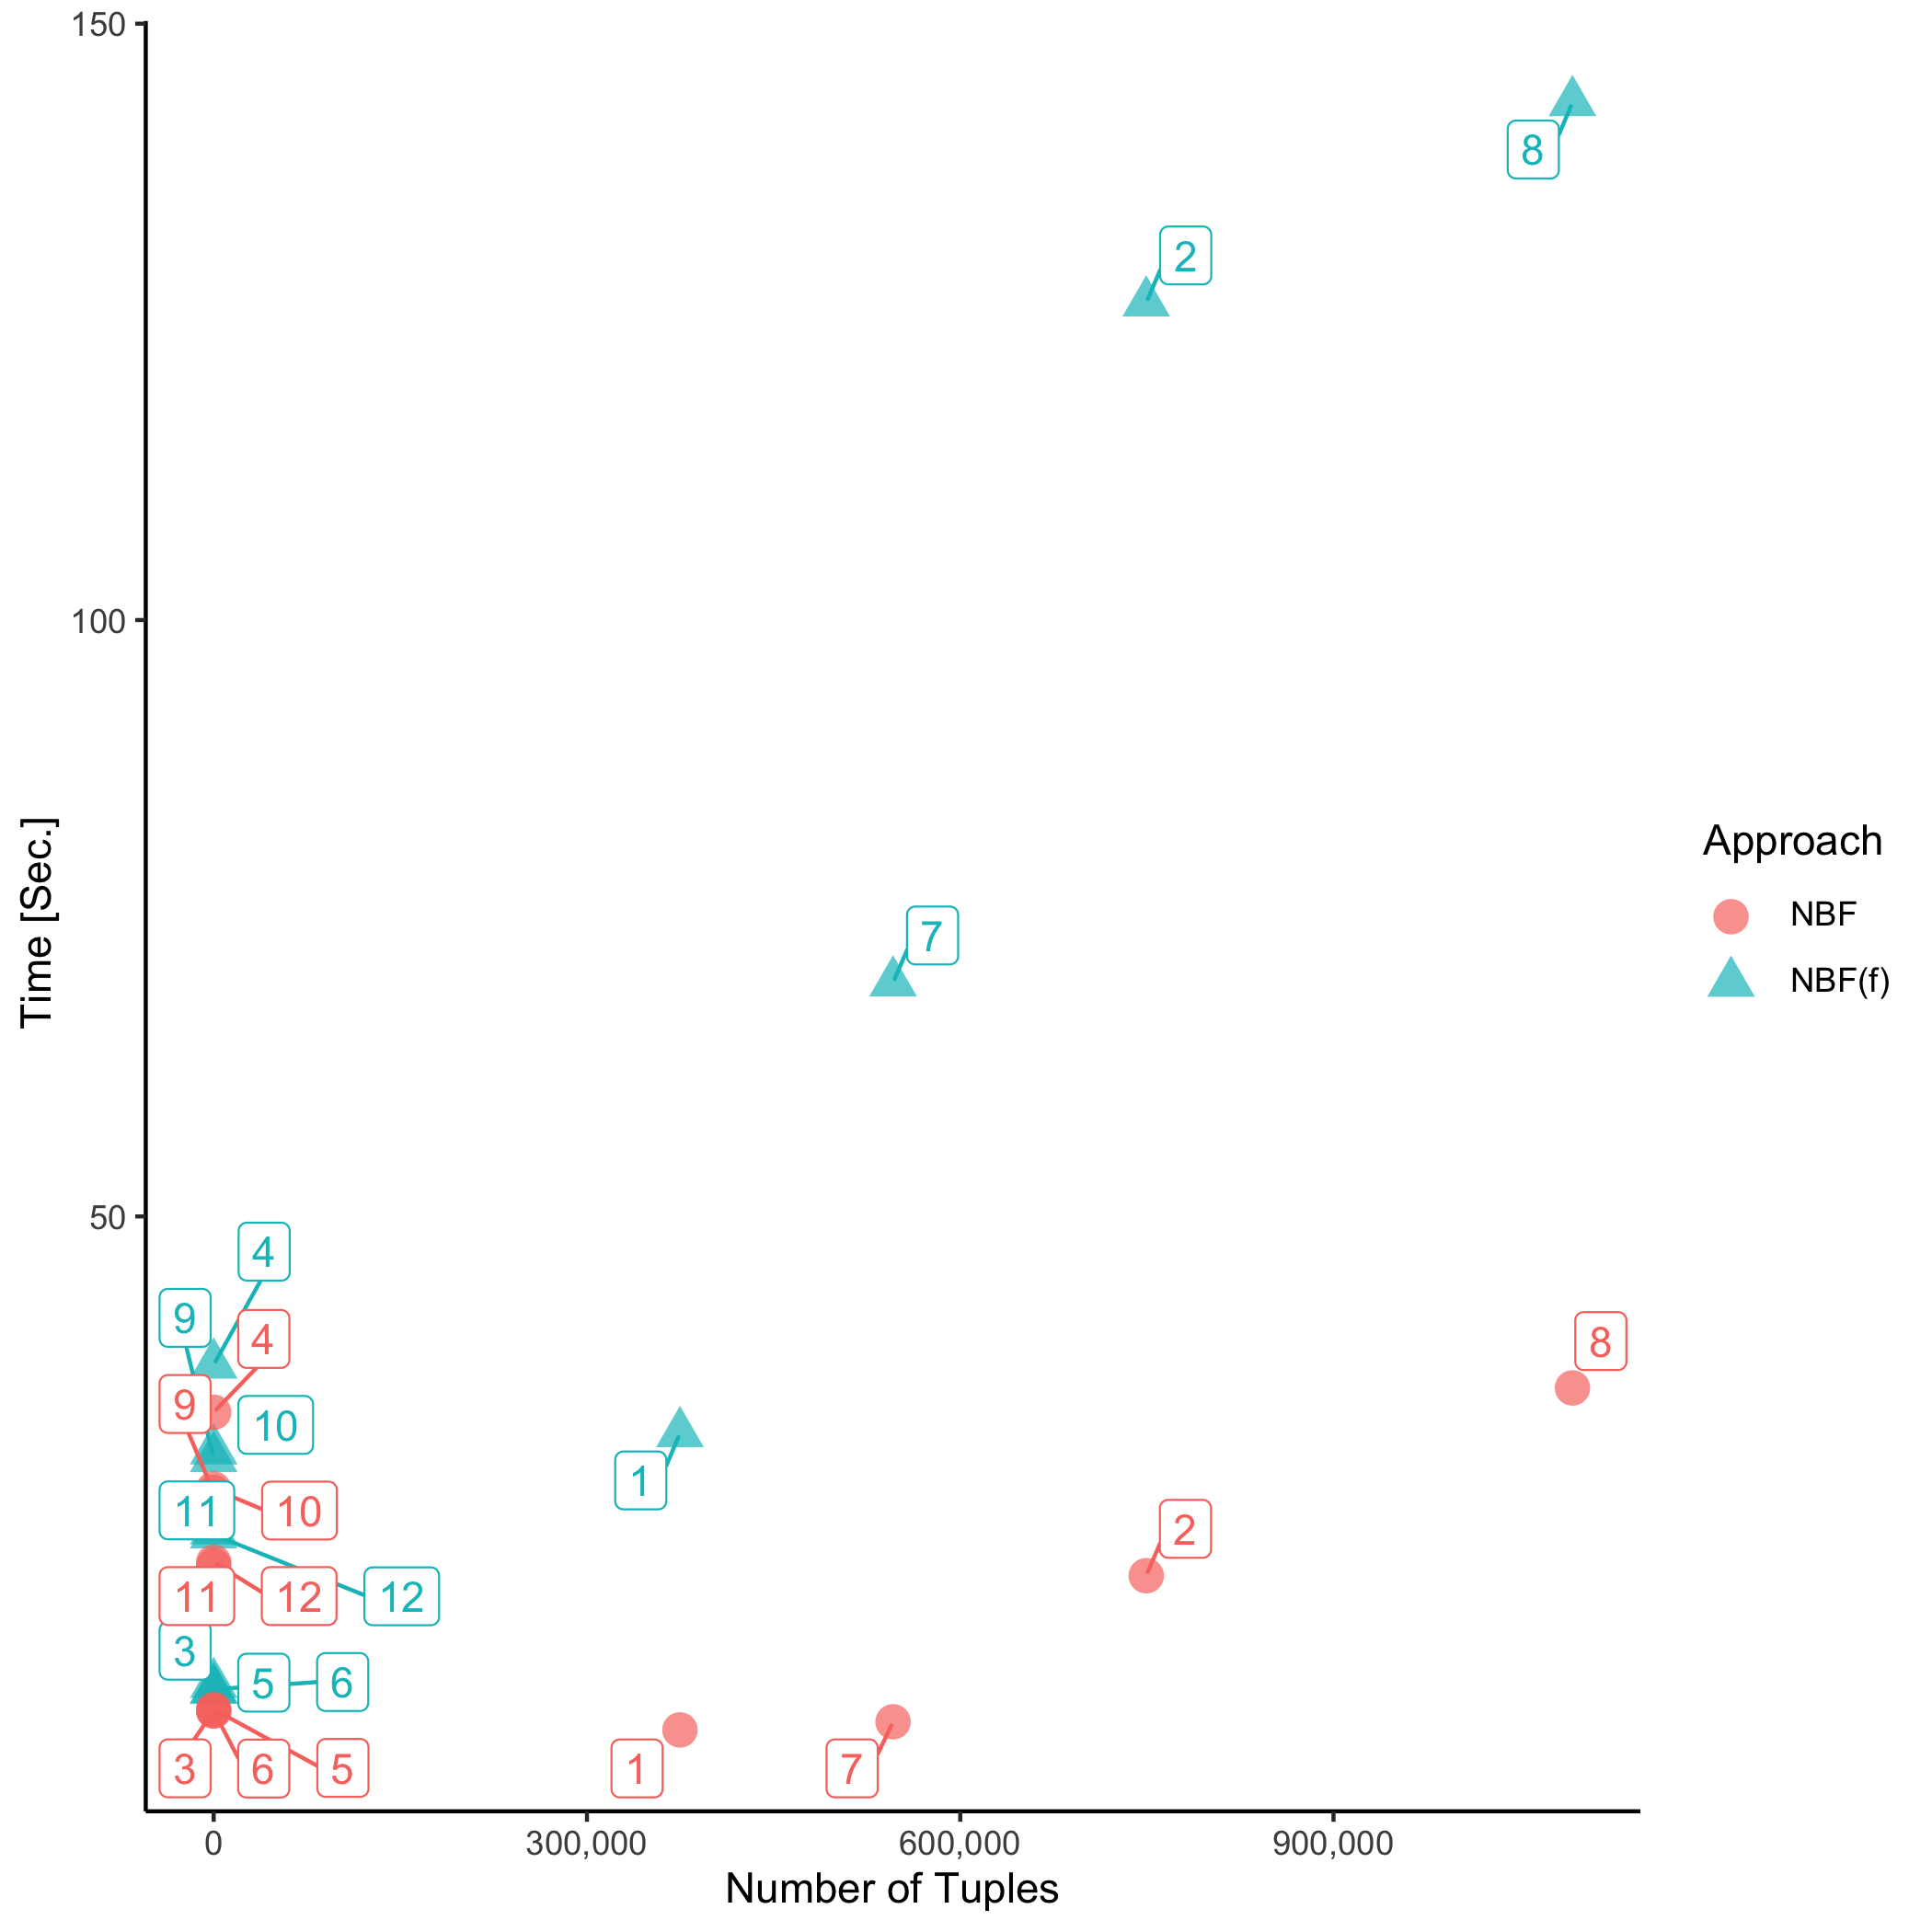
\includegraphics[scale=0.09]{figs/plots/emp-nbf-f-comp-scatter.png}
%        \caption{Lorem ipsum, lorem ipsum,Lorem ipsum, lorem ipsum,Lorem ipsum}
%    \end{subfigure}
%    \caption{Caption place holder}
%\end{figure*}
\begin{figure*}[t!]
    \centering
    \begin{subfigure}[t]{0.5\textwidth}
        \centering
        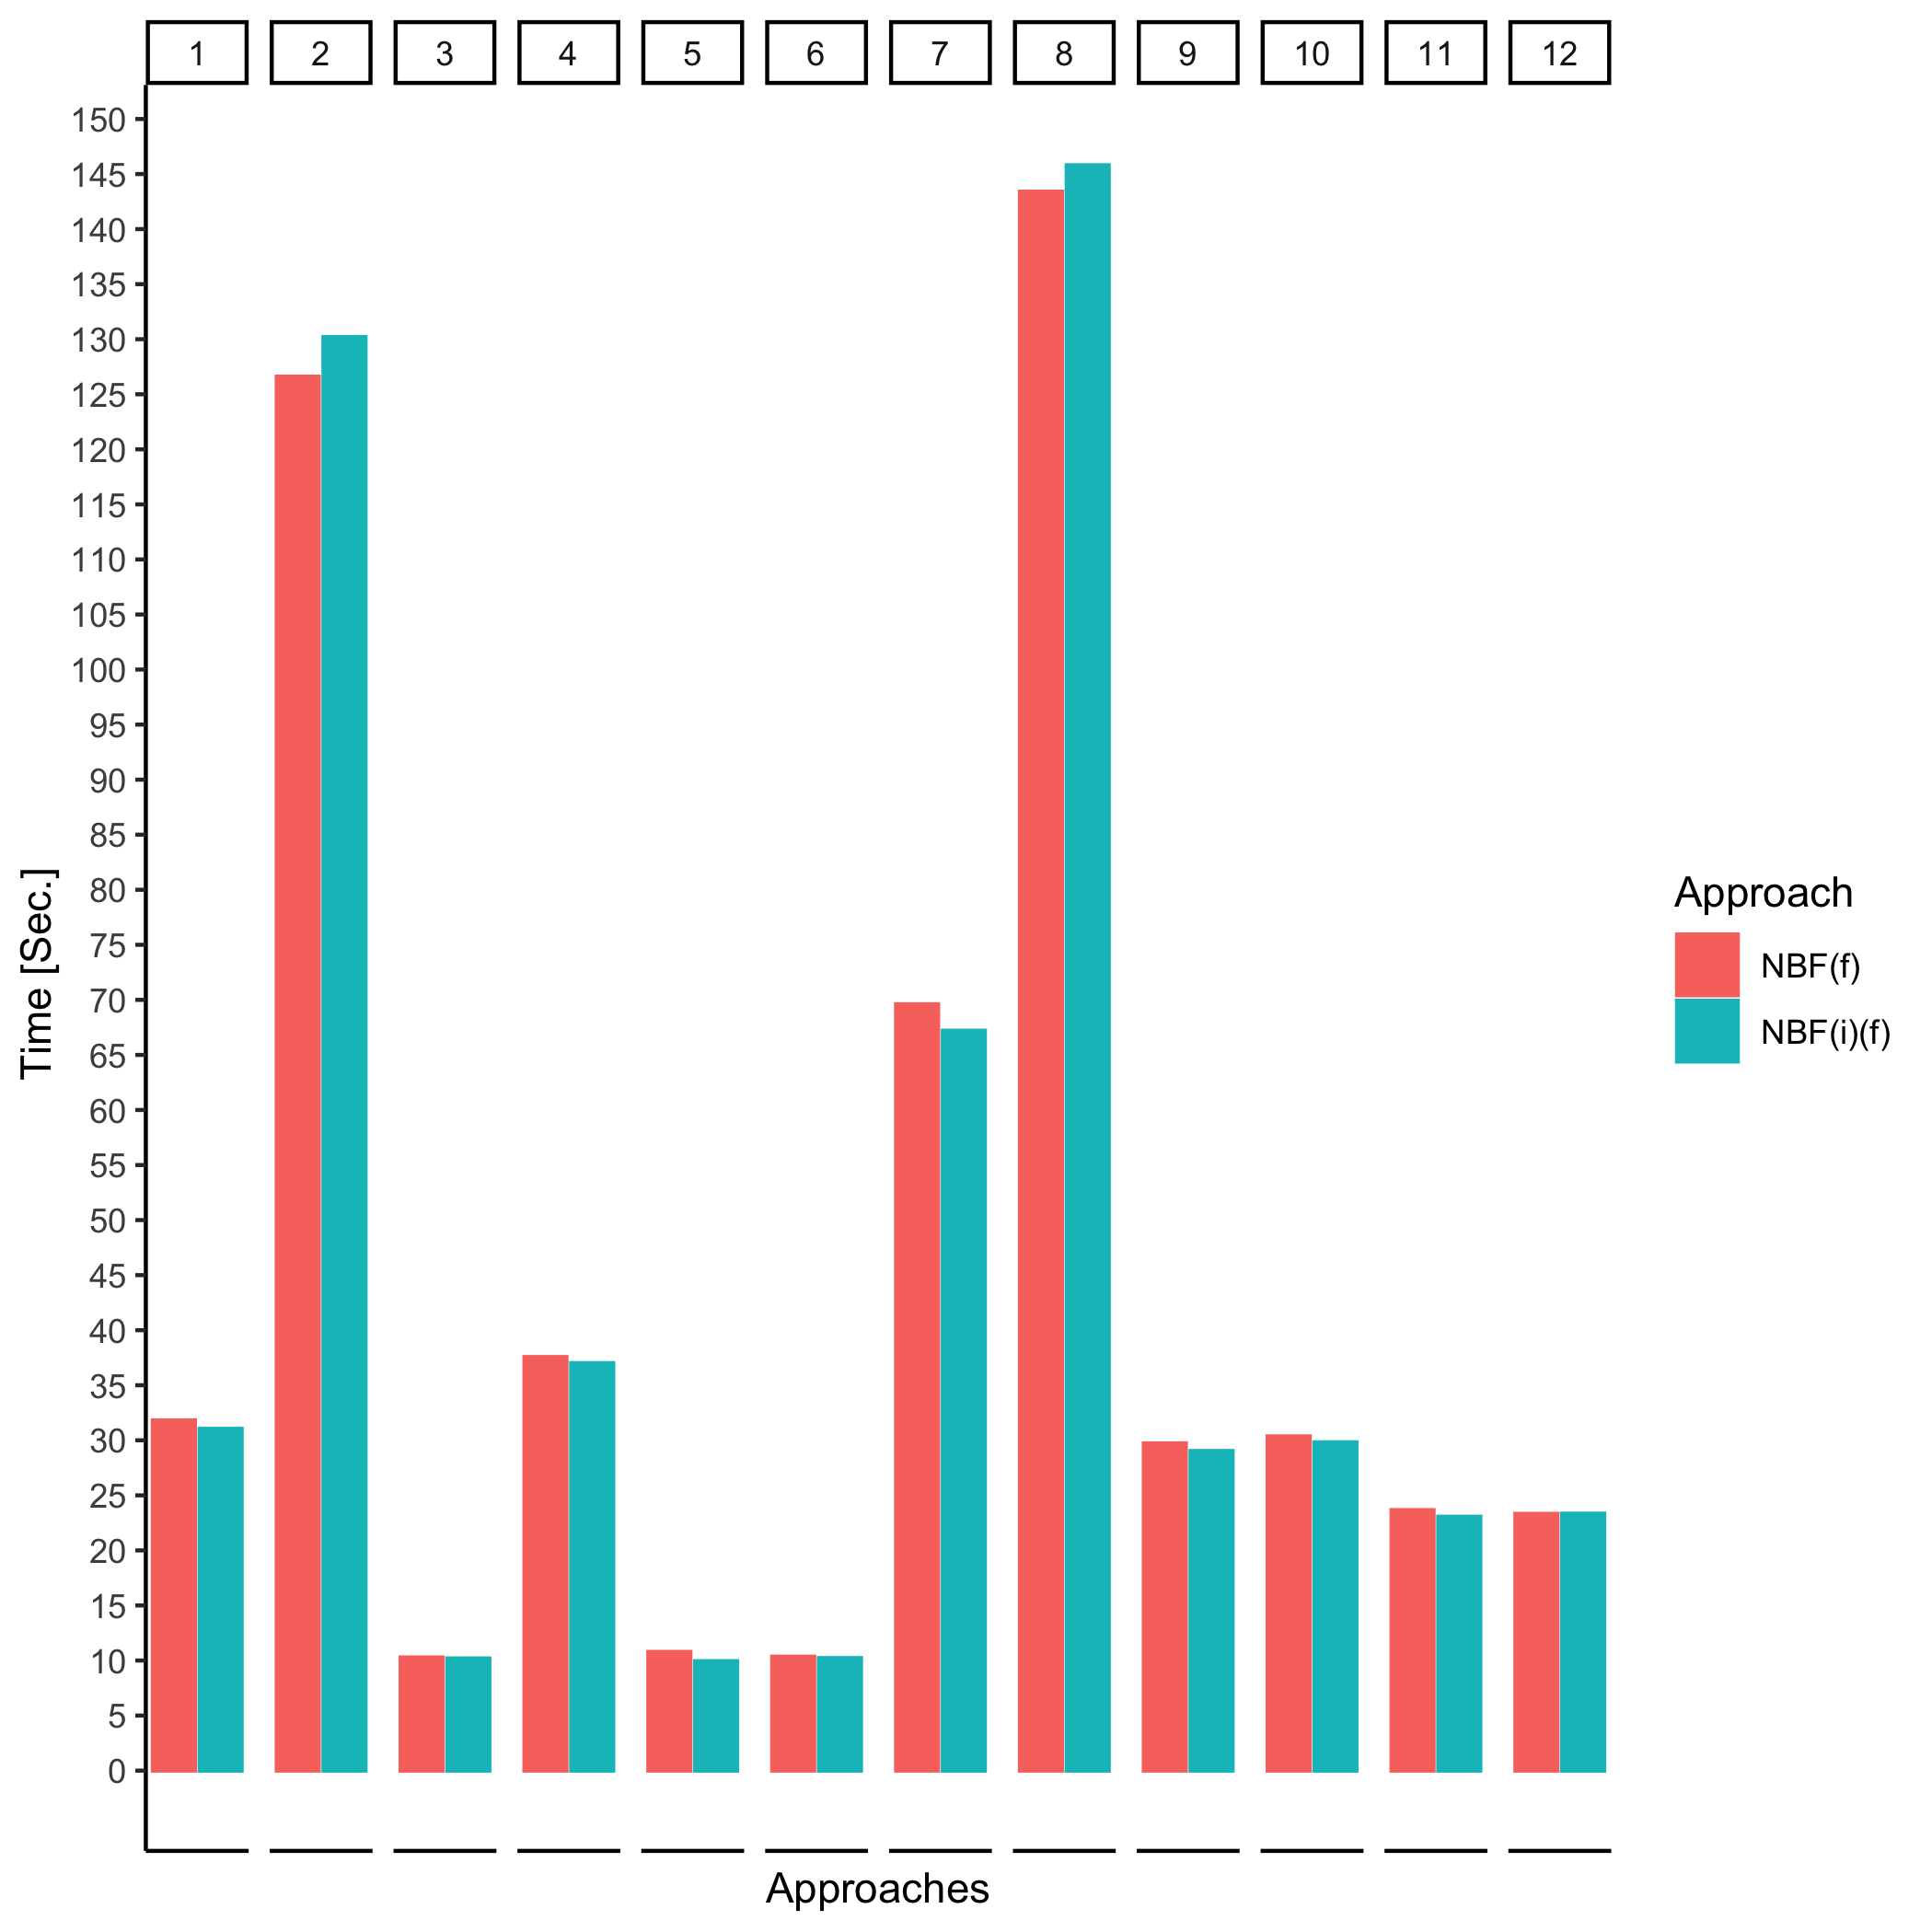
\includegraphics[scale=0.06]{figs/plots/emp-nbf-f.png}
        \caption[Comparison of the \nbff\ and \nbfif\ approaches on the employee VDB]{Comparison of the \nbff\ and \nbfif\ approaches on the employee VDB.}
    \end{subfigure}%
    ~ 
    \begin{subfigure}[t]{0.5\textwidth}
        \centering
        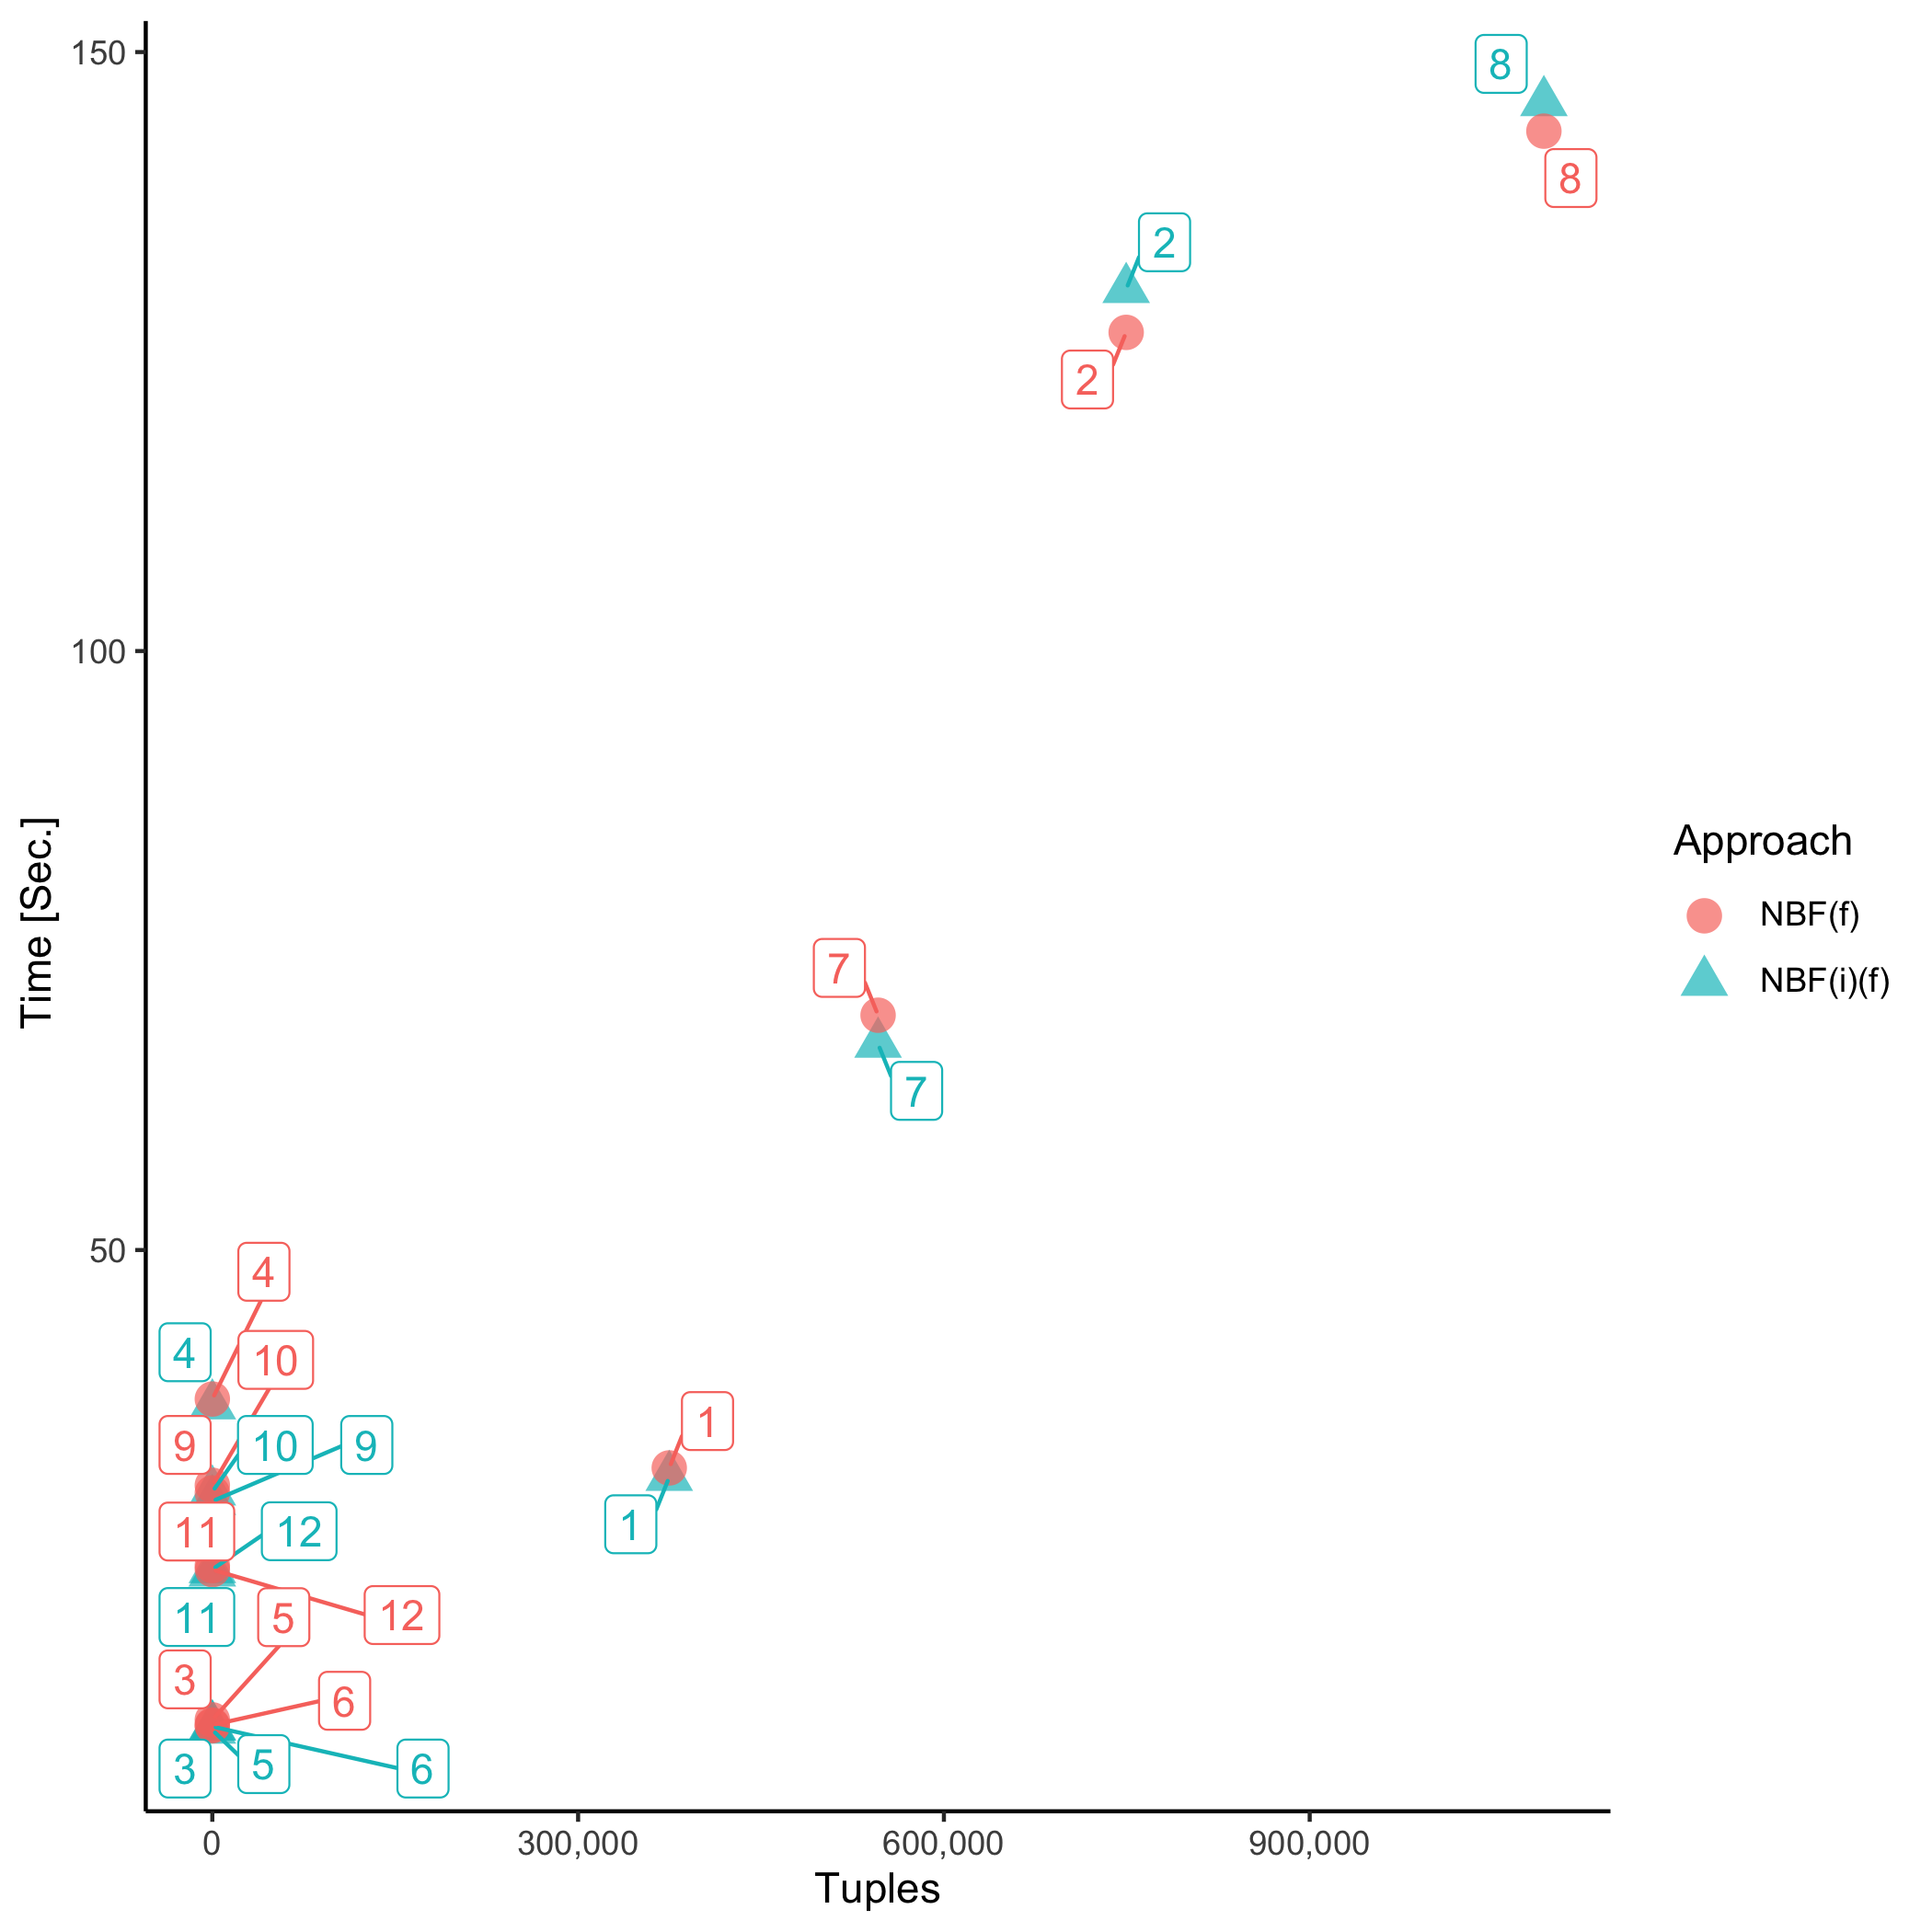
\includegraphics[scale=0.06]{figs/plots/emp-nbf-f-scatter.png}
        \caption[Comparison of the \nbff\ and \nbfif\ approaches on the employee VDB]{Comparison of the \nbff\ and \nbfif\ approaches on the employee VDB.}
    \end{subfigure}\\[1 ex]
    \begin{subfigure}[t]{0.5\textwidth}
        \centering
        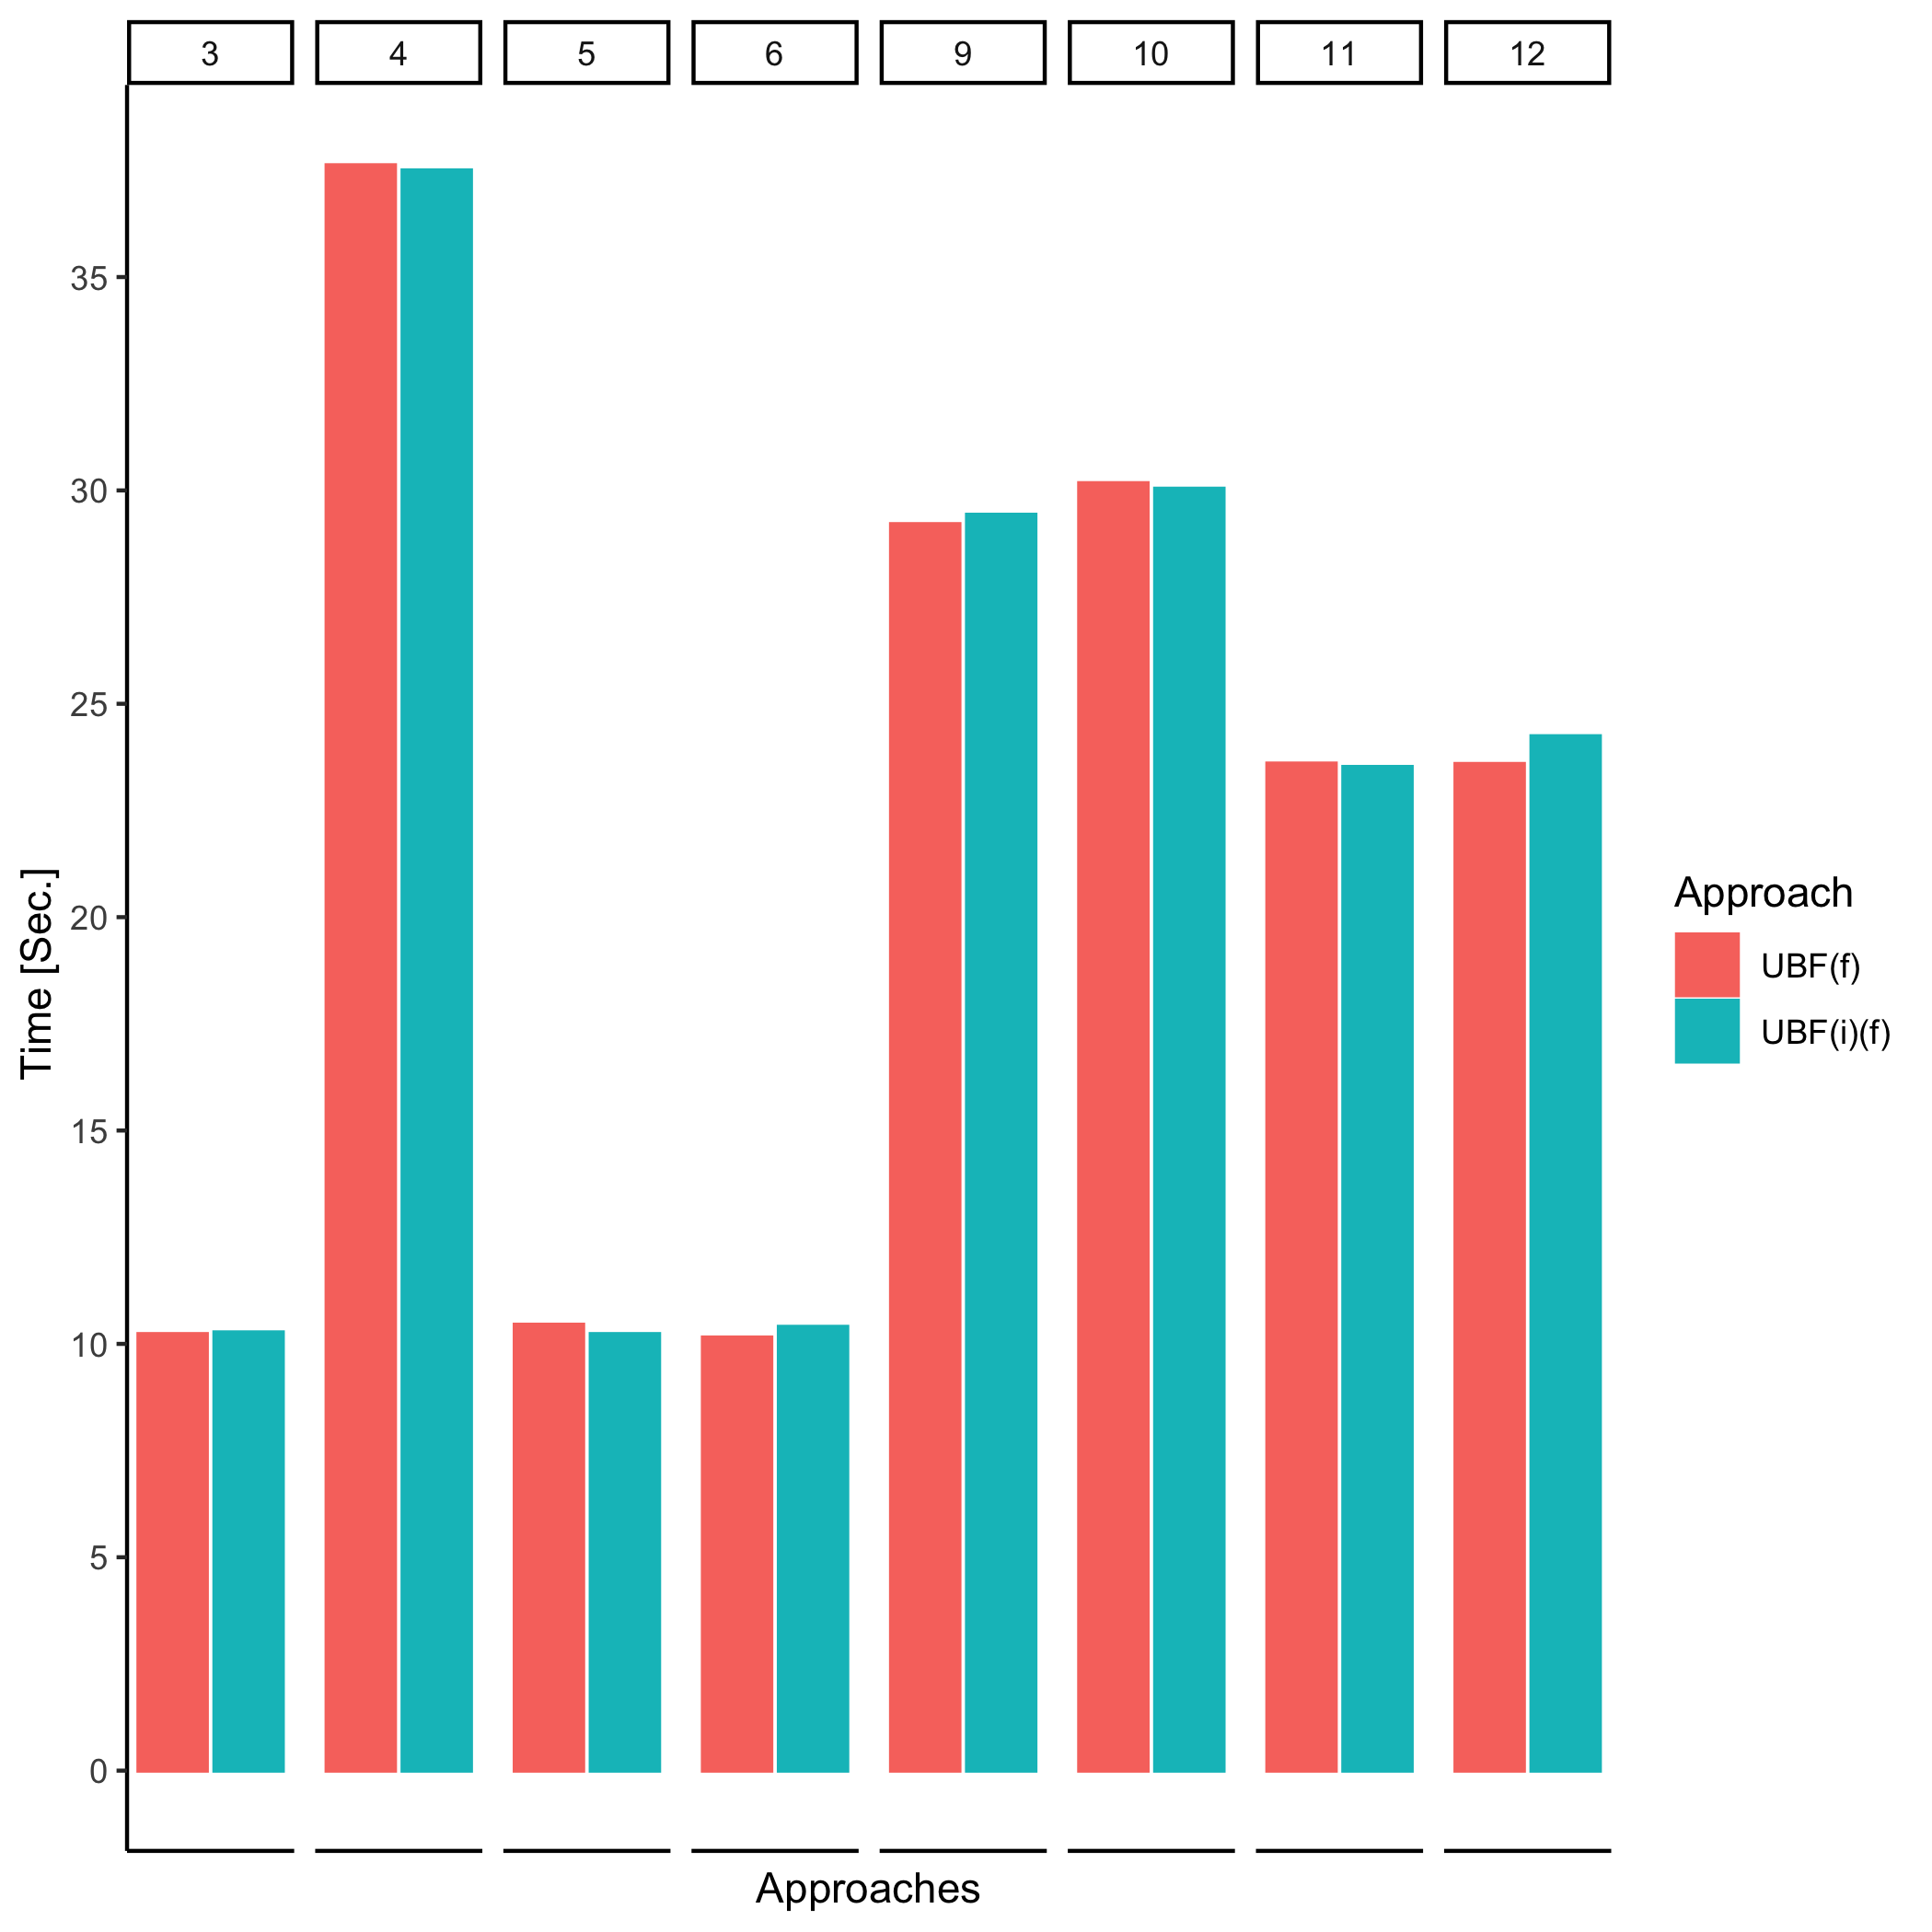
\includegraphics[scale=0.06]{figs/plots/emp-ubf-f.png}
        \caption[Comparison of the \ubff\ and \ubfif\ approaches on the employee VDB]{Comparison of the \ubff\ and \ubfif\ approaches on the employee VDB}
    \end{subfigure}%
    ~ 
    \begin{subfigure}[t]{0.5\textwidth}
        \centering
        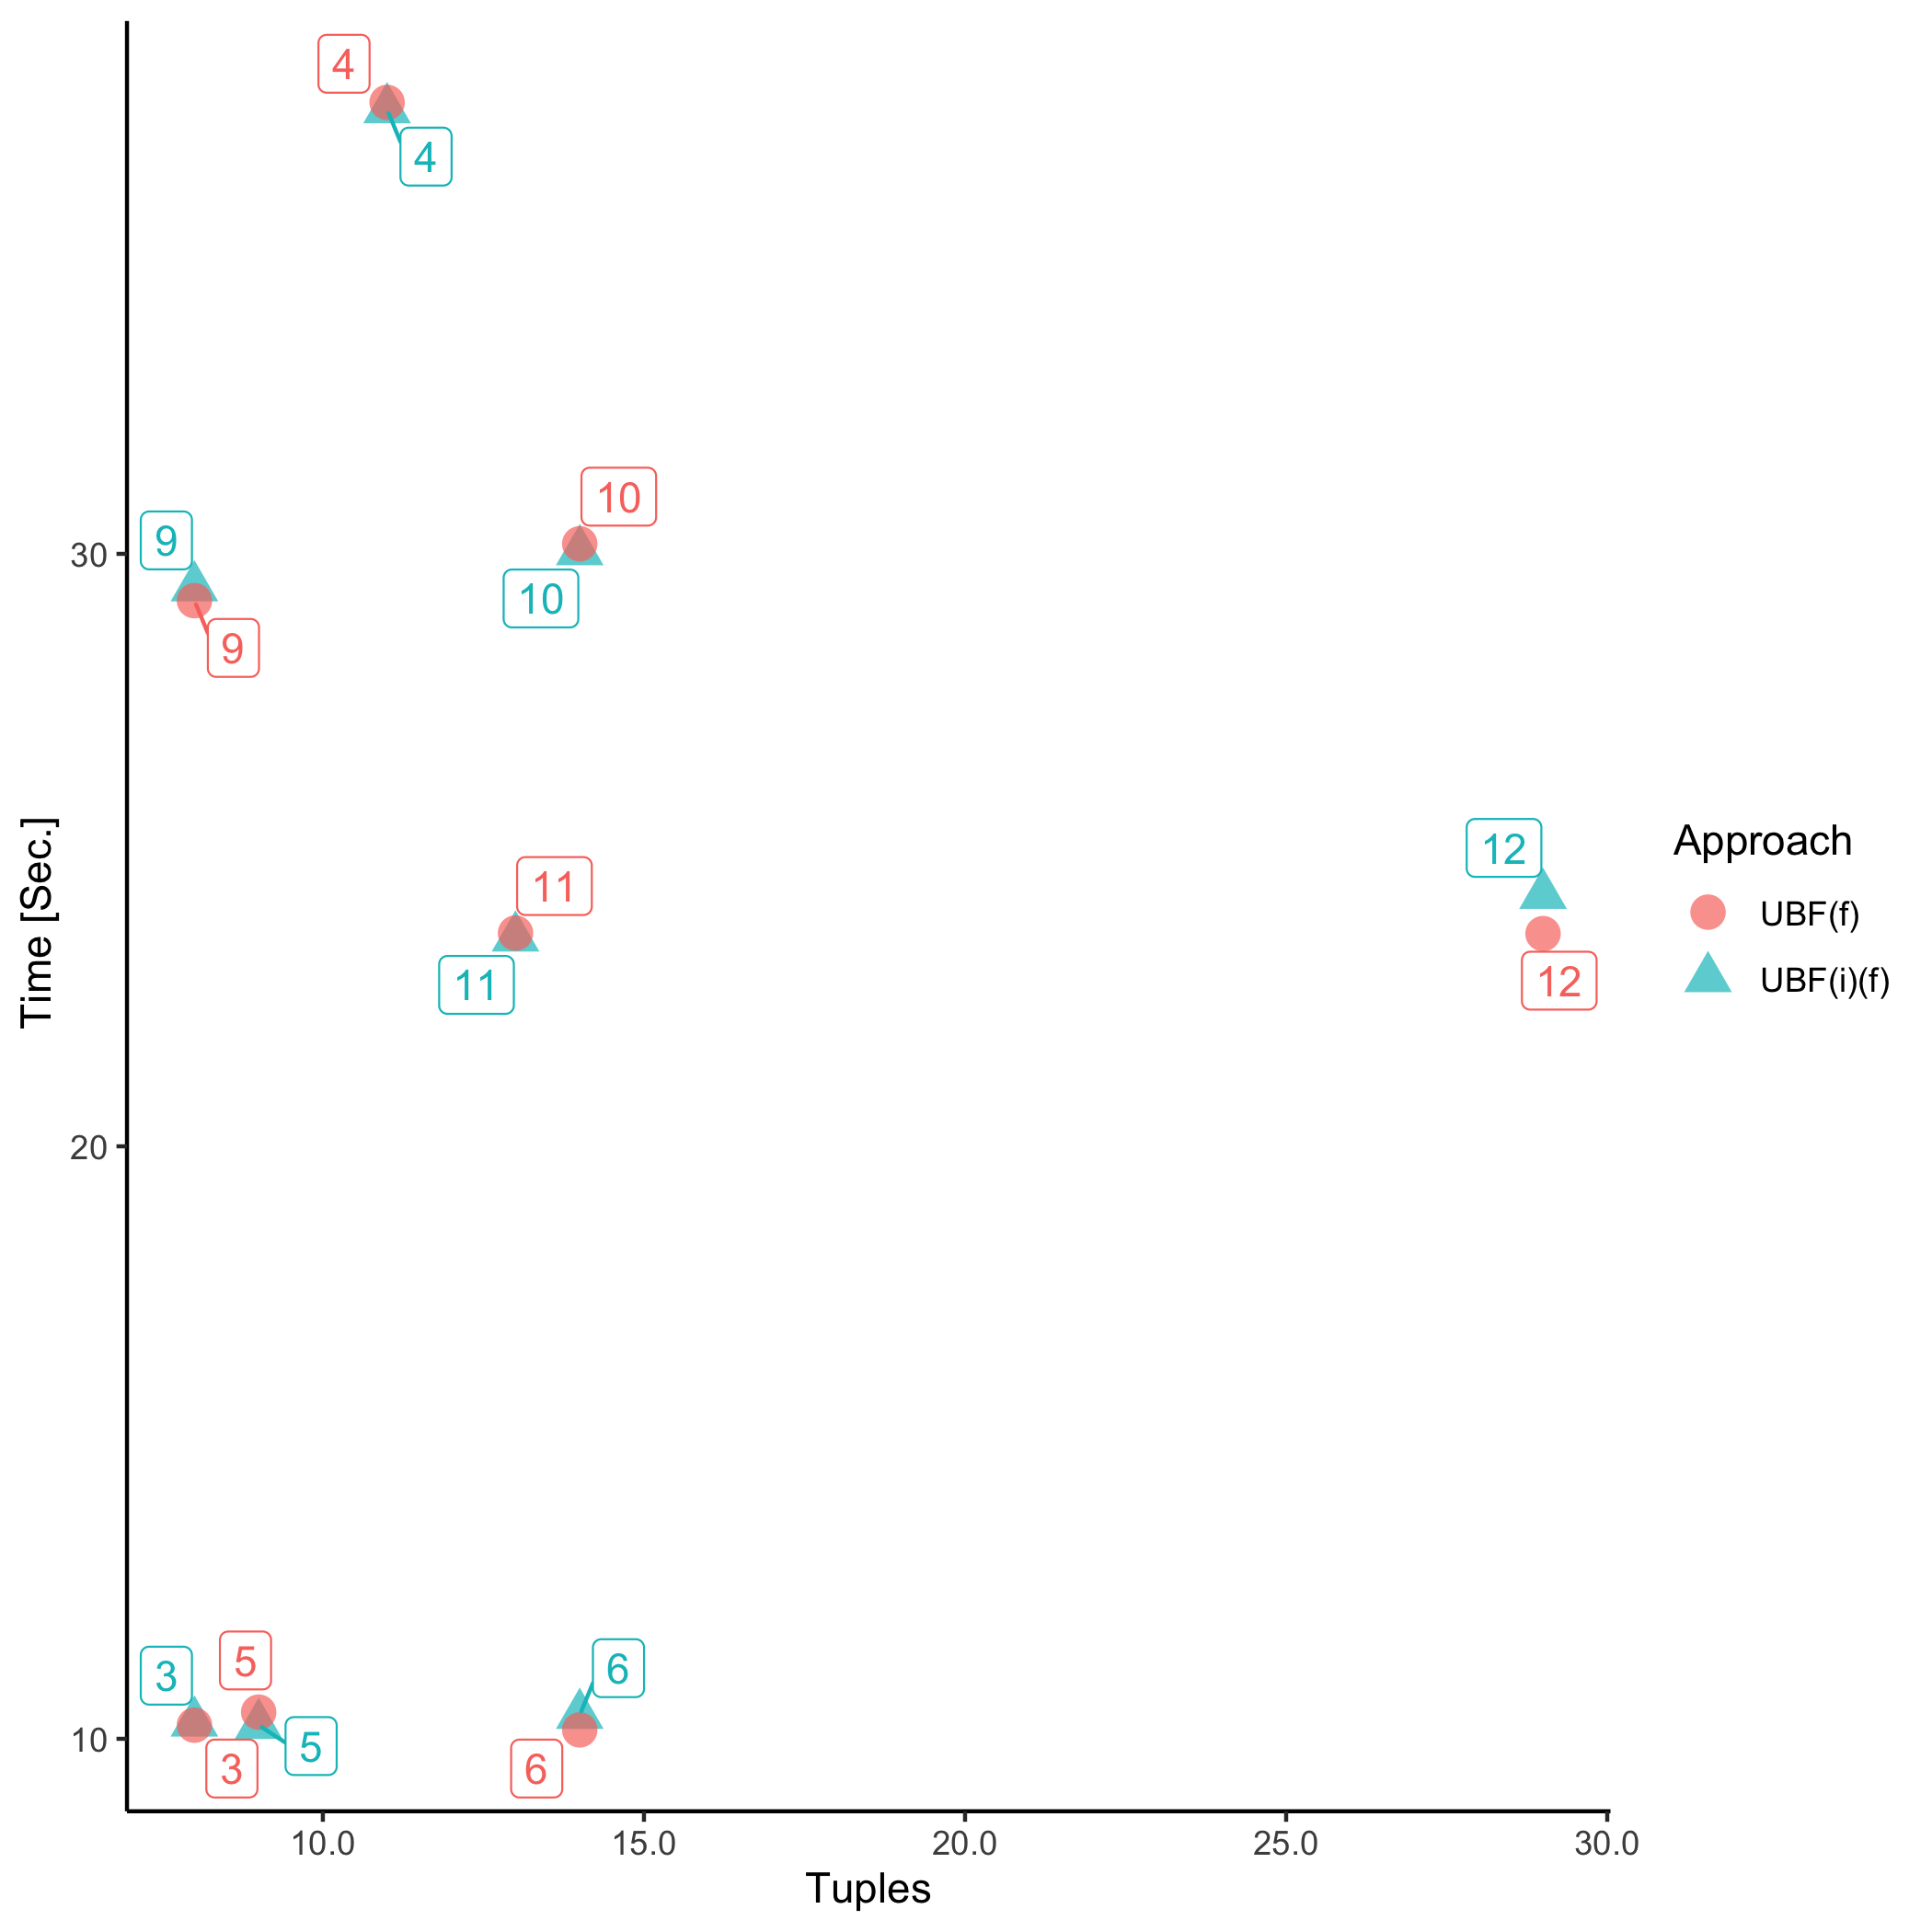
\includegraphics[scale=0.06]{figs/plots/emp-ubf-f-scatter.png}
        \caption[Comparison of the \ubff\ and \ubfif\ approaches on the employee VDB]{Comparison of the \ubff\ and \ubfif\ approaches on the employee VDB}
    \end{subfigure}\\[1 ex]
    \begin{subfigure}[t]{0.5\textwidth}
        \centering
        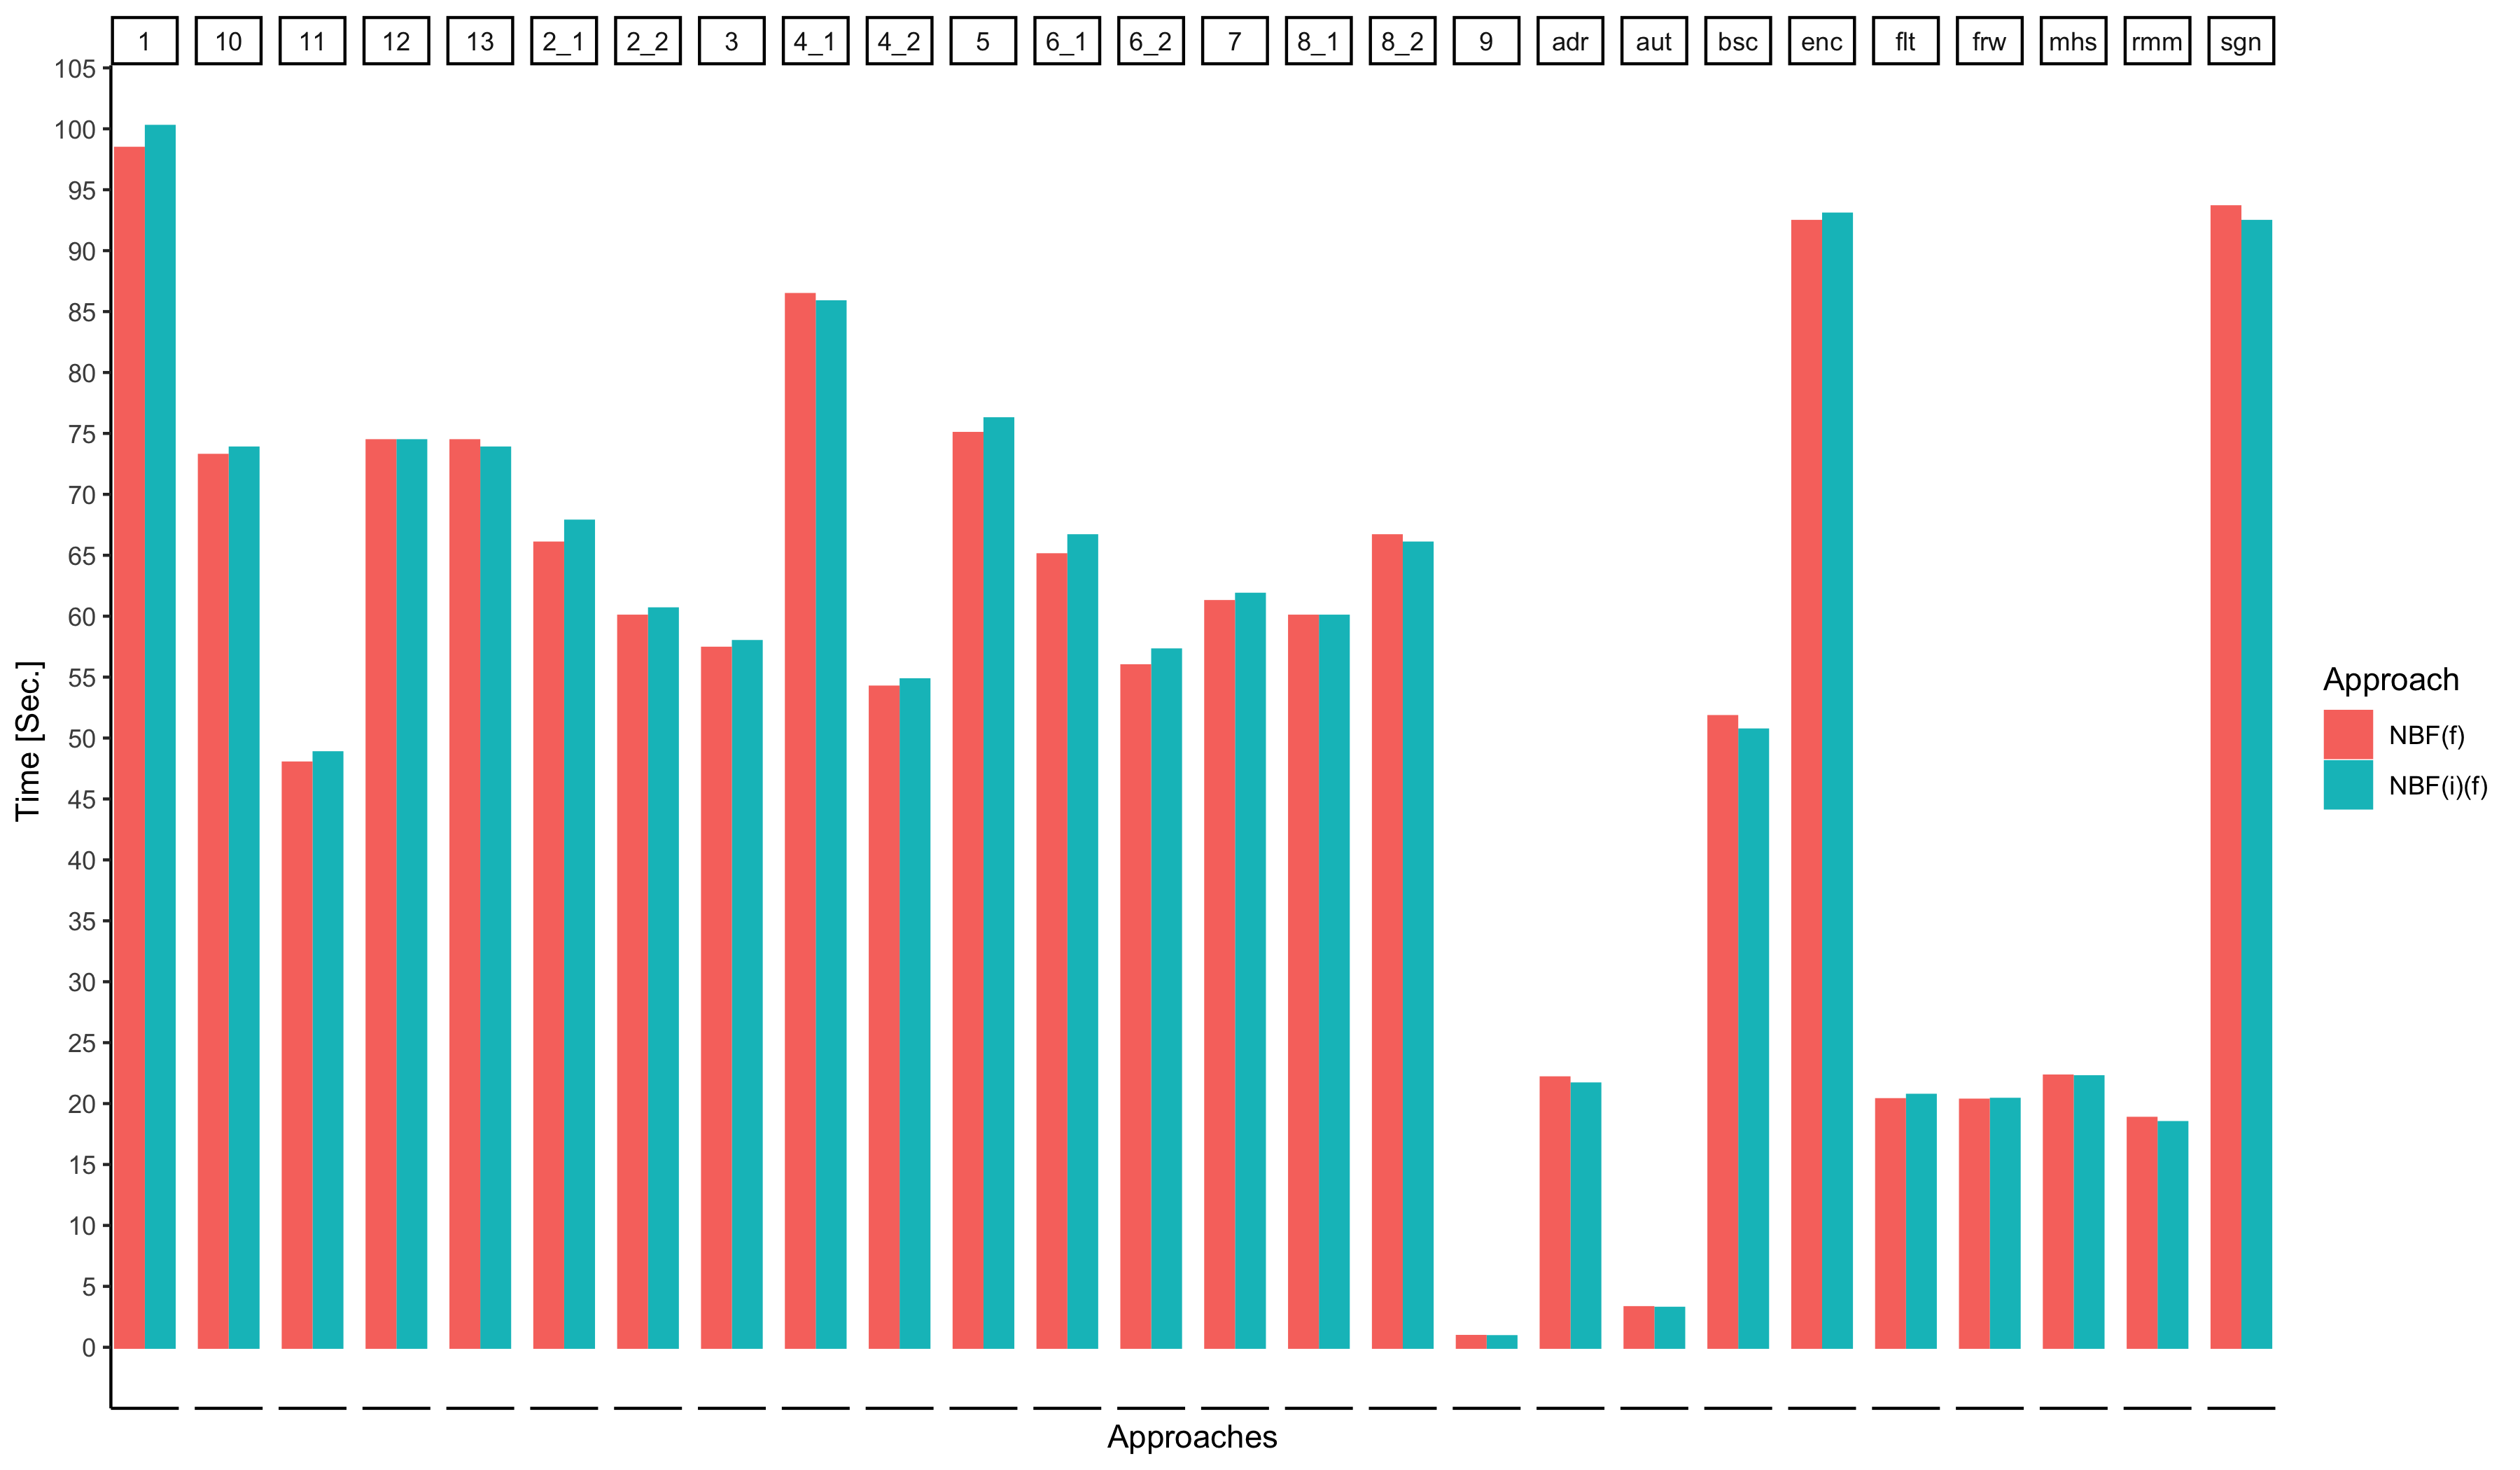
\includegraphics[width=\textwidth]{figs/plots/enron-nbf-f.png}
        \caption[Comparison of the \nbff\ and \nbfif\ approaches on the email VDB]{Comparison of the \nbff\ and \nbfif\ approaches on the email VDB}
    \end{subfigure}%
    ~ 
    \begin{subfigure}[t]{0.5\textwidth}
        \centering
        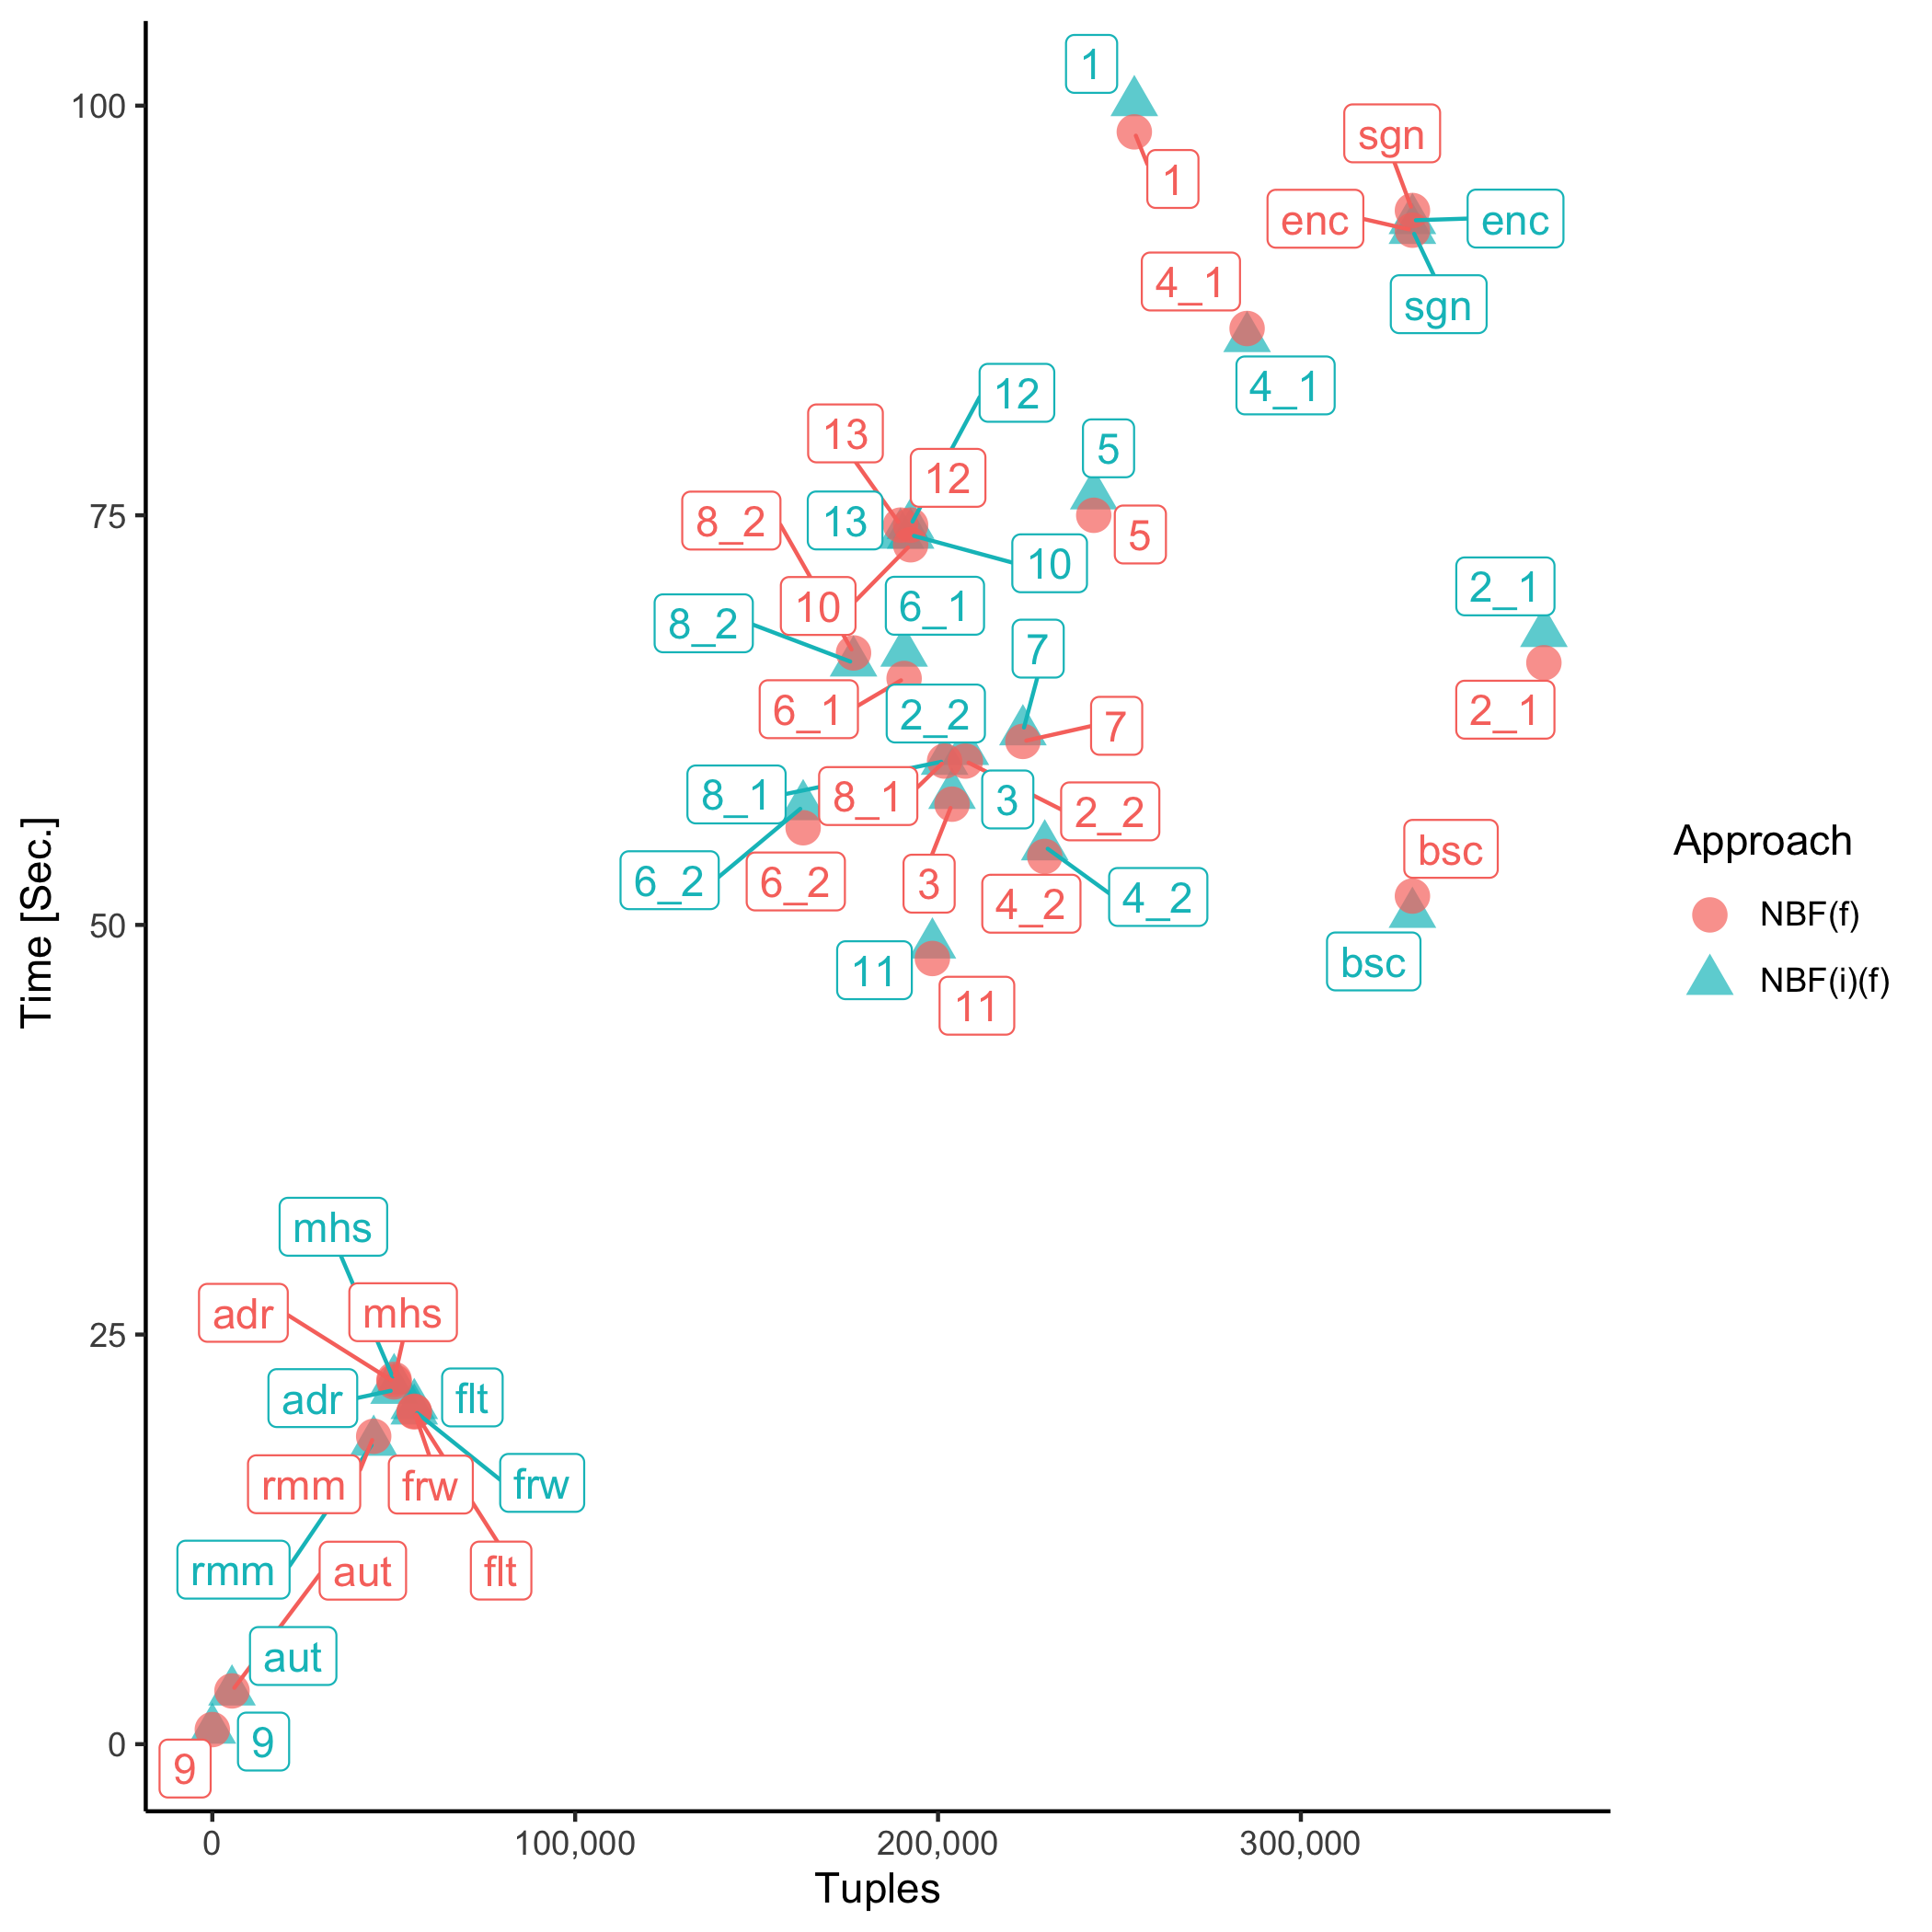
\includegraphics[scale=0.07]{figs/plots/enron-nbf-f-scatter.png}
        \caption[Comparison of the \nbff\ and \nbfif\ approaches on the email VDB]{Comparison of the \nbff\ and \nbfif\ approaches on the email VDB}
    \end{subfigure}
    \caption[The effect of filtering out tuples with unsatisfiable presence conditions when presence conditions are injected into a query in SQL generator approaches]{The effect of filtering out tuples with unsatisfiable presence conditions when presence conditions are injected into a query in  on SQL generator approaches.}
    \label{fig:filter-comp}
\end{figure*}